% This LaTeX document needs to be compiled with XeLaTeX.
\documentclass[
  10
]{article}
\usepackage[margin=2cm,includehead=true,includefoot=true,centering,]{geometry}
\usepackage{xcolor}
\usepackage{ucharclasses}
\usepackage{hyperref}
\usepackage{amsmath,amssymb}
\usepackage{amsfonts}
\usepackage[version=4]{mhchem}
\usepackage{stmaryrd}
\usepackage{bbold}
\usepackage{polyglossia}
\usepackage{fontspec}
\usepackage{ctex}
\usepackage[export]{adjustbox}
\usepackage{tabularx}
\usepackage{booktabs}

\usepackage{setspace}
\setstretch{1.2}

\makeatletter
\@ifundefined{KOMAClassName}{% if non-KOMA class
  \IfFileExists{parskip.sty}{%
    \usepackage{parskip}
  }{% else
    \setlength{\parindent}{0pt}
    \setlength{\parskip}{6pt plus 2pt minus 1pt}}
}{% if KOMA class
  \KOMAoptions{parskip=half}}
\makeatother
\usepackage{color}
\usepackage{fancyvrb}
\newcommand{\VerbBar}{|}
\newcommand{\VERB}{\Verb[commandchars=\\\{\}]}
\DefineVerbatimEnvironment{Highlighting}{Verbatim}{commandchars=\\\{\}}
% Add ',fontsize=\small' for more characters per line
\newenvironment{Shaded}{}{}
\newcommand{\AlertTok}[1]{\textcolor[rgb]{1.00,0.00,0.00}{\textbf{#1}}}
\newcommand{\AnnotationTok}[1]{\textcolor[rgb]{0.38,0.63,0.69}{\textbf{\textit{#1}}}}
\newcommand{\AttributeTok}[1]{\textcolor[rgb]{0.49,0.56,0.16}{#1}}
\newcommand{\BaseNTok}[1]{\textcolor[rgb]{0.25,0.63,0.44}{#1}}
\newcommand{\BuiltInTok}[1]{\textcolor[rgb]{0.00,0.50,0.00}{#1}}
\newcommand{\CharTok}[1]{\textcolor[rgb]{0.25,0.44,0.63}{#1}}
\newcommand{\CommentTok}[1]{\textcolor[rgb]{0.38,0.63,0.69}{\textit{#1}}}
\newcommand{\CommentVarTok}[1]{\textcolor[rgb]{0.38,0.63,0.69}{\textbf{\textit{#1}}}}
\newcommand{\ConstantTok}[1]{\textcolor[rgb]{0.53,0.00,0.00}{#1}}
\newcommand{\ControlFlowTok}[1]{\textcolor[rgb]{0.00,0.44,0.13}{\textbf{#1}}}
\newcommand{\DataTypeTok}[1]{\textcolor[rgb]{0.56,0.13,0.00}{#1}}
\newcommand{\DecValTok}[1]{\textcolor[rgb]{0.25,0.63,0.44}{#1}}
\newcommand{\DocumentationTok}[1]{\textcolor[rgb]{0.73,0.13,0.13}{\textit{#1}}}
\newcommand{\ErrorTok}[1]{\textcolor[rgb]{1.00,0.00,0.00}{\textbf{#1}}}
\newcommand{\ExtensionTok}[1]{#1}
\newcommand{\FloatTok}[1]{\textcolor[rgb]{0.25,0.63,0.44}{#1}}
\newcommand{\FunctionTok}[1]{\textcolor[rgb]{0.02,0.16,0.49}{#1}}
\newcommand{\ImportTok}[1]{\textcolor[rgb]{0.00,0.50,0.00}{\textbf{#1}}}
\newcommand{\InformationTok}[1]{\textcolor[rgb]{0.38,0.63,0.69}{\textbf{\textit{#1}}}}
\newcommand{\KeywordTok}[1]{\textcolor[rgb]{0.00,0.44,0.13}{\textbf{#1}}}
\newcommand{\NormalTok}[1]{#1}
\newcommand{\OperatorTok}[1]{\textcolor[rgb]{0.40,0.40,0.40}{#1}}
\newcommand{\OtherTok}[1]{\textcolor[rgb]{0.00,0.44,0.13}{#1}}
\newcommand{\PreprocessorTok}[1]{\textcolor[rgb]{0.74,0.48,0.00}{#1}}
\newcommand{\RegionMarkerTok}[1]{#1}
\newcommand{\SpecialCharTok}[1]{\textcolor[rgb]{0.25,0.44,0.63}{#1}}
\newcommand{\SpecialStringTok}[1]{\textcolor[rgb]{0.73,0.40,0.53}{#1}}
\newcommand{\StringTok}[1]{\textcolor[rgb]{0.25,0.44,0.63}{#1}}
\newcommand{\VariableTok}[1]{\textcolor[rgb]{0.10,0.09,0.49}{#1}}
\newcommand{\VerbatimStringTok}[1]{\textcolor[rgb]{0.25,0.44,0.63}{#1}}
\newcommand{\WarningTok}[1]{\textcolor[rgb]{0.38,0.63,0.69}{\textbf{\textit{#1}}}}
\usepackage{longtable,booktabs,array}
\newcounter{none} % for unnumbered tables
\usepackage{multirow}
\usepackage{calc} % for calculating minipage widths
% Correct order of tables after \paragraph or \subparagraph
\usepackage{etoolbox}
\makeatletter
\patchcmd\longtable{\par}{\if@noskipsec\mbox{}\fi\par}{}{}
\makeatother
% Allow footnotes in longtable head/foot
\IfFileExists{footnotehyper.sty}{\usepackage{footnotehyper}}{\usepackage{footnote}}
\makesavenoteenv{longtable}
\usepackage{graphicx}
\makeatletter
\newsavebox\pandoc@box
\newcommand*\pandocbounded[1]{% scales image to fit in text height/width
  \sbox\pandoc@box{#1}%
  \Gscale@div\@tempa{\textheight}{\dimexpr\ht\pandoc@box+\dp\pandoc@box\relax}%
  \Gscale@div\@tempb{\linewidth}{\wd\pandoc@box}%
  \ifdim\@tempb\p@<\@tempa\p@\let\@tempa\@tempb\fi% select the smaller of both
  \ifdim\@tempa\p@<\p@\scalebox{\@tempa}{\usebox\pandoc@box}%
  \else\usebox{\pandoc@box}%
  \fi%
}
% Set default figure placement to htbp
\def\fps@figure{htbp}
\makeatother
\setlength{\emergencystretch}{3em} % prevent overfull lines
\providecommand{\tightlist}{%
  \setlength{\itemsep}{0pt}\setlength{\parskip}{0pt}}


\hypersetup{colorlinks=true, linkcolor=blue, filecolor=magenta, urlcolor=cyan,}
\urlstyle{same}

\usepackage{colortbl}
\definecolor{table-row-color}{HTML}{999999}
\definecolor{table-rule-color}{HTML}{999999}
%\arrayrulecolor{black!40}
\arrayrulecolor{table-rule-color}     % color of \toprule, \midrule, \bottomrule
\setlength{\aboverulesep}{0pt}
\setlength{\belowrulesep}{0pt}


\setotherlanguages{english}
\IfFontExistsTF{Source Han Serif CN}
{\newfontfamily\chinesefont{Source Han Serif CN}}
{\IfFontExistsTF{Noto Serif CJK SC}
  {\newfontfamily\chinesefont{Noto Serif CJK SC}}
  {\IfFontExistsTF{SimSun}
    {\newfontfamily\chinesefont{SimSun}}
    {\IfFontExistsTF{FangSong}
      {\newfontfamily\chinesefont{FangSong}}
      {\newfontfamily\chinesefont{Arial Unicode MS}}
}}}
\IfFontExistsTF{Times New Roman}
{\newfontfamily\englishfont{Times New Roman}}
{\IfFontExistsTF{Liberation Serif}
  {\newfontfamily\englishfont{Liberation Serif}}
  {\IfFontExistsTF{DejaVu Serif}
    {\newfontfamily\englishfont{DejaVu Serif}}
    {\newfontfamily\englishfont{Arial}}
}}


\author{}
\date{}

\begin{document}


O P E N C L AW O R A N G E PA P E R · 橙 ⽪ 书

\section{OpenClaw}\label{openclaw}

\section{橙皮书}\label{ux6a59ux76aeux4e66}

从入门到精通，涵盖架构原理、部署方案、渠道接入、Skills系统、模型配置、安全与成本的一站式参考手册。

信息来源：OpenClaw官方文档·GitHub仓库·社区调研

文档版本：v1.4.0

适用版本：v2026.3.13

发布时间：2026-03-24 (build \#1)

涵盖内容：架构原理·部署指南·渠道接入·Skills系统·模型配置·安全与成本·生态全景

\section{花叔}\label{ux82b1ux53d4}

B站：AI进化论-花生·YouTube：AI进化论-花生·公众号：花叔

知识星球：AI编程·从入门到精通

本文档在ClaudeCode辅助下整理编写，内容的准确性与时效性仅供参考。

如有勘误或建议，欢迎关注公众号「花叔」反馈交流。

配套视频教程：B站「OpenClaw从0到1」·后续更新：飞书文档

\section{目录}\label{ux76eeux5f55}

Table of Contents

\section{Part 1: 认识 OpenClaw · Meet
OpenClaw}\label{part-1-ux8ba4ux8bc6-openclaw-meet-openclaw}

01 OpenClaw 是什么 What is OpenClaw

02 发展简史 History

03 创始人故事 The Creator

04 为什么这么火 Why So Popular

\section{Part 2: 技术架构 ·
Architecture}\label{part-2-ux6280ux672fux67b6ux6784-architecture}

05 整体架构 Architecture Overview

06 记忆系统 Memory System

07 Agent 工作区 Agent Workspace

08 Session 与用户识别 Sessions \& Authentication

09 设计哲学 Design Philosophy

\section{Part 3: 部署方案 ·
Deployment}\label{part-3-ux90e8ux7f72ux65b9ux6848-deployment}

10 部署方式总览 Deployment Overview

11 本地安装 Local Installation

12 Docker 部署 Docker Deployment

13 国内云厂商一键部署 Cloud Deployment in China

14 首次配置 Initial Configuration

\section{Part 4: 渠道接入 · Channel
Integration}\label{part-4-ux6e20ux9053ux63a5ux5165-channel-integration}

15 渠道概览 Channel Overview

16 国际平台接入 International Platforms

17 国内平台接入 Chinese Platforms

18 远程访问 Remote Access

\section{Part 5: Skills 系统 · Skills
System}\label{part-5-skills-ux7cfbux7edf-skills-system}

19 Skills 工作原理 How Skills Work

20 ClawHub 与技能生态 ClawHub \& Skill Ecosystem

21 热门 Skills 推荐 Top Skills

22 自建 Skill 指南 Create Your Own Skill

23 Skills 安全 Skill Security

\section{Part 6: 模型配置 · Model
Configuration}\label{part-6-ux6a21ux578bux914dux7f6e-model-configuration}

24 模型提供商总览 Provider Overview

25 国际模型配置 International Models

26 国产模型配置 Chinese Models

27 本地模型与推荐方案 Local Models \& Recommendations

\section{Part 7: 安全与成本 · Security \&
Cost}\label{part-7-ux5b89ux5168ux4e0eux6210ux672c-security-cost}

28 安全模型 Security Model

29 已知安全事件 Security Incidents

30 成本控制 Cost Control

\section{Part 8: 生态与社区 · Ecosystem \&
Community}\label{part-8-ux751fux6001ux4e0eux793eux533a-ecosystem-community}

31 养虾文化 Lobster Culture

32 平替产品 Alternatives

33 vs Claude Code Comparison with Claude Code

34 国内生态 China Ecosystem

35 国产Claw产品选购指南 Claw Products in China

\section{附录 · Appendix}\label{ux9644ux5f55-appendix}

A 常见问题 FAQ Frequently Asked Questions

B 命令速查表 Command Cheat Sheet

C 资源链接 Resources \& Links

\section{01 OpenClaw 是什么}\label{openclaw-ux662fux4ec0ux4e48}

一个开源、自托管的AI
Agent系统，让AI从「聊天工具」变成「能自主执行任务的数字员工」。

如果你用过ChatGPT，你会知道它本质上是一个问答系统：你问，它答。OpenClaw不一样。它是一个AI
Agent平台，能连接 \(^ { 2 0 + }\)
消息渠道（WhatsApp、Telegram、飞书、钉钉、Discord等），主动执行任务、管理你的日程、处理邮件、操作浏览器、调用各种工具。

换句话说，ChatGPT是「顾问」，OpenClaw是「员工」。

与ChatGPT的核心区别

{\def\LTcaptype{none} % do not increment counter
\begin{longtable}[]{@{}|l|l|l|@{}}
\toprule\noalign{}
\endhead
\bottomrule\noalign{}
\endlastfoot
\hline
维度 & ChatGPT & OpenClaw \\
\hline
交互模式 & 你问它答 & 自主执行任务 \\
\hline
运行环境 & 网页/App & 自托管服务器，接入20+消息平台 \\
\hline
可扩展性 & GPTs商店 & ClawHub技能市场（13,729个Skills） \\
\hline
数据控制 & 数据在OpenAI & 完全本地，你拥有所有数据 \\
\hline
模型选择 & 仅GPT系列 & Claude / GPT / DeepSeek / Gemini /
Ollama本地模型 \\
\hline
开源 & 否 & MIT License，完全开源 \\
\hline
\end{longtable}
}

{\def\LTcaptype{none} % do not increment counter
\begin{longtable}[]{@{}|l|l|@{}}
\toprule\noalign{}
\endhead
\bottomrule\noalign{}
\endlastfoot
\hline
指标 & 数据 \\
\hline
GitHub Stars & 330,000+ (GitHub历史增速第一，已先后超越React与Linux) \\
\hline
Forks & 64,300+ \\
\hline
贡献者 & 1,075+ \\
\hline
ClawHub Skills & 13,700+ \\
\hline
内置Skills & 55个 \\
\hline
支持消息渠道 & 20+ (WhatsApp / Telegram / Discord / Slack / 飞书 / 钉钉
/ 浏览器等) \\
\hline
最新版本 & v2026.3.13 (2026-03-14发布) \\
\hline
\end{longtable}
}

句话理解OpenClaw：它是一个开源的「个人AI操作系统」，你可以在自己的服务器上运行它，通过任何即时通讯工具跟它交互，让它帮你处理生活和工作中的各种任务。吉祥物是一只龙虾，中文社区称使用OpenClaw为「养虾」。

\section{02 发展简史}\label{ux53d1ux5c55ux7b80ux53f2}

从一个人的周末项目，到不到5个月成为GitHub全球第一。

{\def\LTcaptype{none} % do not increment counter
\begin{longtable}[]{@{}|l|l|@{}}
\toprule\noalign{}
\endhead
\bottomrule\noalign{}
\endlastfoot
\hline
时间 & 事件 \\
\hline
2025年11月 & ClawdBot诞生。奥地利开发者Peter
Steinberger作为周末项目发布。名字致敬Anthropic的Claude(Claw=爪子),选了龙虾作为吉祥物。 \\
\hline
2026年1月中旬 & 爆发式增长。72小时内获得6万Stars,某天单日增长9,000
Stars。 \\
\hline
2026年1月27日 &
Anthropic商标警告。因名称与Claude过于相似,被迫改名为Moltbot(Molt=龙虾蜕壳)。 \\
\hline
2026年1月30日 & 再次改名OpenClaw。强调开源属性,保留龙虾主题。 \\
\hline
2026年2月初 & 安全危机。CVE-2026-25253 RCE漏洞被发现(CVSS
8.8/10),13.5万暴露实例中5万+可被直接攻击。同期ClawHavoc供应链攻击爆发,ClawHub约12\%的Skills被确认为恶意。 \\
\hline
2026年2月初 &
谷歌封号风波。谷歌大规模封禁OpenClaw用户账号,引发社区震动。 \\
\hline
2026年2月14日 & 创始人加入OpenAI。Peter
Steinberger宣布加入OpenAI,项目移交开源基金会运营。OpenAI赞助但项目保持独立。 \\
\hline
2026年3月3日 &
登顶GitHub。v2026.3.2发布,Stars超过250K,正式超越React成为GitHub全球第一软件项目。 \\
\hline
2026年3月7-8日 & v2026.3.7「史诗级更新」。89次提交,Context
Engine插件化、GPT-5.4原生支持、分布式频道绑定。Stars达278,932。深圳龙岗AI局发布OpenClaw支持政策征求意见稿。 \\
\hline
2026年3月9日 &
v2026.3.8安全加固版。新增ACP身份验证、本地备份工具,12+安全补丁。同日工信部和CNCERT发布OpenClaw安全风险预警。Stars突破280,000。 \\
\hline
2026年3月12-13日 &
v2026.3.11+v2026.3.12连续发布。3.11修复WebSocket跨站劫持漏洞,改善本地Ollama集成体验。3.12推出
Dashboard v2全新控制台、/fast
快速模式、本地模型插件化架构(Ollama/vLLM/SGLang),设备配对改用Ephemeral
Token。 \\
\hline
2026年3月14日 & v2026.3.13浏览器自动化升级。支持Chrome
DevTools远程附着已登录浏览器会话,发布BrowserRelay
Chrome扩展,Stars持续增长超越Linux成为GitHub历史第一。 \\
\hline
2026年3月16日 &
智谱发布GLM-5-Turbo。历史上第一个从训练阶段就专为OpenClaw场景优化的基座模型,主打工具调用、长链执行、持久任务,128K输出/200K上下文,支持MCP协议,目前实验性闭源发布。 \\
\hline
\end{longtable}
}

\section{核心建议}\label{ux6838ux5fc3ux5efaux8bae}

OpenClaw先后超越React和Linux，成为GitHub历史上增速最快的开源项目。React用了超过10年才达到23万Stars，Linux用了更长时间，而OpenClaw不到5个月就完成了这一切。

\section{03 创始人故事}\label{ux521bux59cbux4ebaux6545ux4e8b}

Peter Steinberger：从周末项目到全球最火开源项目，再到加入OpenAI。

\section{从一个人到一个社区}\label{ux4eceux4e00ux4e2aux4ebaux5230ux4e00ux4e2aux793eux533a}

Peter
Steinberger是一位奥地利开发者，在iOS和macOS开发圈有很高的知名度。2025年11月的一个周末，他写了一个能连接即时通讯平台的AI助手小工具，取名ClawdBot。

他大概没有想到，这个周末项目会在两个月后成为GitHub上增长最快的开源项目。到2026年3月，他个人在这个项目上提交了11,684次commit，贡献者超过1,075人。

\section{加入OpenAI}\label{ux52a0ux5165openai}

2026年2月14日，Peter宣布加入OpenAI。Sam
Altman亲自发推欢迎，称他为「genius」。

这个决定引发了社区的广泛讨论。但Peter做了几件事来消除担忧：

OpenClaw转为开源基金会运营，保持项目独立

OpenAI作为赞助商之一（与Vercel、Blacksmith、Convex并列），但不控制项目方向

OpenAI承诺让他继续投入OpenClaw的开发

Peter的原话：「I'm a builder at heart\ldots{} What I want is to change
the world, not build a large
company.」（我骨子里是个建造者。我想改变世界，而不是建一家大公司。）

\section{关于名字的故事}\label{ux5173ux4e8eux540dux5b57ux7684ux6545ux4e8b}

ClawdBot这个名字来自对Anthropic
Claude的致敬（Claw=爪子），所以选了龙虾作为吉祥物。Anthropic的商标警告迫使他改名为Moltbot（Molt=龙虾蜕壳），三天后又改为OpenClaw，强调开源属性。虽然经历了两次改名，龙虾的形象始终保留，也成了整个社区的文化符号。

\section{04 为什么这么火}\label{ux4e3aux4ec0ux4e48ux8fd9ux4e48ux706b}

不到5个月从0到33万Stars，OpenClaw的爆火不只是技术层面的事。

增长数据

{\def\LTcaptype{none} % do not increment counter
\begin{longtable}[]{@{}|l|l|l|@{}}
\toprule\noalign{}
\endhead
\bottomrule\noalign{}
\endlastfoot
\hline
时间节点 & Stars & 备注 \\
\hline
2025年11月 & 0 & 项目创建 \\
\hline
2026年1月中旬 & 60,000+ & 72小时爆发增长 \\
\hline
2026年2月中旬 & 145,000+ & Peter加入OpenAI \\
\hline
2026年3月1日 & 241,000+ & 逼近React \\
\hline
2026年3月3日 & 250,000+ & 超越React，GitHub第一 \\
\hline
2026年3月8日 & 278,932 & v2026.3.7发布 \\
\hline
2026年3月9日 & 280,000+ & v2026.3.8发布，超越React \\
\hline
2026年3月24日 & 330,000+ & 3周增长80K，超越Linux成为GitHub历史第一 \\
\hline
2026年3月14日 & 超越 Linux & v2026.3.13发布，写本书时的最新数据 \\
\hline
\end{longtable}
}

某天单日增长9,000Stars。这个数字意味着平均每10秒就有一个开发者点下Star。超越React之后，OpenClaw继续增长，再次超越Linux，成为GitHub有史以来增速最快的开源项目。

\section{「养虾」文化现象}\label{ux517bux867eux6587ux5316ux73b0ux8c61}

因为吉祥物是龙虾，中文社区将运行OpenClaw称为「养虾」，用户自称「养虾人」。「你养龙虾了吗？」成了AI圈的问候语。这种有趣的文化标签降低了传播门槛，让一个技术项目有了社交货币的属性。

2026年3月6日，深圳腾讯云总部近千人排队体验OpenClaw安装。3月8日，深圳龙岗区AI（机器人）局发布了OpenClaw使用支持措施的征求意见稿。一个开源项目能引发地方政府的政策关注，这在国内并不多见。

\section{Moltbook：AI
Agent的社交网络}\label{moltbookai-agentux7684ux793eux4ea4ux7f51ux7edc}

OpenClaw生态中衍生出了一个叫Moltbook的社交平台，专供AIAgent使用。截至2026年2月底的数据：

{\def\LTcaptype{none} % do not increment counter
\begin{longtable}[]{@{}|l|l|@{}}
\toprule\noalign{}
\endhead
\bottomrule\noalign{}
\endlastfoot
\hline
指标 & 数据 \\
\hline
注册AI Agent & 32,912 \\
\hline
子社区 & 2,364 \\
\hline
帖子 & 3,130 \\
\hline
评论 & 22,046 \\
\hline
\end{longtable}
}

数千个OpenClaw实例在上面发帖、评论、讨论哲学问题。这可能是AIAgent从「工具」走向「社会化存在」的第一个大规模实验场。

\section{热门玩法}\label{ux70edux95e8ux73a9ux6cd5}

\section{赚钱型}\label{ux8d5aux94b1ux578b}

在Polymarket上用AI进行预测市场交易，已有OpenClaw月入数万美元的案例

ClawWork项目：「OpenClaw作为你的AI Coworker，11小时赚\$15K」

\section{生活助手型}\label{ux751fux6d3bux52a9ux624bux578b}

接管邮件、日历、消息管理

浏览网页、填表、数据抽取

文件读写、Shell命令执行

\section{社交养成型}\label{ux793eux4ea4ux517bux6210ux578b}

在Moltbook上给Agent设定名字和性格，观察其「社交行为

Agent之间的交互形成了一种「赛博养成」文化

\section{企业部署型}\label{ux4f01ux4e1aux90e8ux7f72ux578b}

国内用户大量接入飞书、钉钉、企业微信、QQ

已有专门的openclaw-china插件套件，支持三步Docker部署

\section{注意}\label{ux6ce8ux610f}

OpenClaw的火爆背后也有阴影：ClawHub 13,729个Skills中超过 \(5 0 \%\)
被判定为垃圾/重复/低质量，396个被标记为恶意。一觉醒来收到\$1,100API账单的恐怖故事在社区频繁出现。CVE-2026-25253RCE漏洞曾让13.5万个暴露实例面临风险。「养虾」虽然火，但安全和成本控制是你必须认真对待的事。

\section{05 整体架构}\label{ux6574ux4f53ux67b6ux6784}

OpenClaw 采用 Gateway-Node-Channel 三层架构，以 WebSocket
为通信总线，将控制平面、设备执行与消息渠道解耦。

\section{三层架构 Gateway · Node ·
Channel}\label{ux4e09ux5c42ux67b6ux6784-gateway-node-channel}

\pandocbounded{
\includegraphics[keepaspectratio,alt={image}]{images/a381c92e0cbef50801dfcacc4b37df432d7492c51cdc85d68b3825d1651c1d71.jpg}}

{\def\LTcaptype{none} % do not increment counter
\begin{longtable}[]{@{}|l|l|l|@{}}
\toprule\noalign{}
\endhead
\bottomrule\noalign{}
\endlastfoot
\hline
层级 & 职责 & 关键细节 \\
\hline
Gateway & 中央控制平面，维护WebSocket服务、管理Session、调度Agent &
默认绑定ws://127.0.0.1:18789，每台主机一个实例 \\
\hline
Node & 设备端执行节点，负责本地操作 & camera（摄像头）、screen
recording（录屏）、system.run（系统命令）等 \\
\hline
Channel & 消息渠道接入层，连接20+即时通讯平台 &
WhatsApp、Telegram、Discord、Slack、飞书、钉钉等 \\
\hline
\end{longtable}
}

\section{Loopback-First 设计 Security by
Default}\label{loopback-first-ux8bbeux8ba1-security-by-default}

Gateway 默认只绑定 localhost
（127.0.0.1），所有流量在本地回环。这意味着：

不开放任何外网端口，天然安全

同一台机器上的 Node 直接通过 WebSocket 连接 Gateway

需要远程访问时，通过 Tailscale Serve/Funnel 暴露，不直接暴露端口

\section{核心建议}\label{ux6838ux5fc3ux5efaux8bae-1}

每台主机只运行一个Gateway实例。这是因为WhatsAppWeb等渠道需要独占会话，多实例会导致登录冲突。

\section{通信流程}\label{ux901aux4fe1ux6d41ux7a0b}

一条消息从用户发出到Agent回复，完整路径如下：

\pandocbounded{
\includegraphics[keepaspectratio,alt={image}]{images/33c6b31643704e18d41ea6156ab006cdd6d589f41f497802adcc9883c4cf6946.jpg}}

Gateway 作为 24/7 运行的 daemon，持续监听所有已连接的 Channel。它不像
CLI Agent 那样会话结束就丢失上下文，而是长驻运行，积累记忆。

\section{06 记忆系统}\label{ux8bb0ux5fc6ux7cfbux7edf}

记忆是OpenClaw区别于普通Chatbot的核心能力。四层记忆从不可变的身份内核到实时对话，构建完整的上下文连续性。

\section{四层记忆架构}\label{ux56dbux5c42ux8bb0ux5fc6ux67b6ux6784}

{\def\LTcaptype{none} % do not increment counter
\begin{longtable}[]{@{}|l|l|l|l|l|l|l|l|@{}}
\toprule\noalign{}
\endhead
\bottomrule\noalign{}
\endlastfoot
\hline
& SOUL 不可变内核 & → & TOOLS 动态工具 & → & USER 语义长期记忆 & → &
Session 实时情景 \\
\hline
层级 & \multicolumn{2}{l}{%
存储位置} & 生命周期 & \multicolumn{4}{l@{}}{%
说明} \\
\hline
SOUL & \multicolumn{2}{l}{%
SOUL.md} & 永久不可变 & \multicolumn{4}{l@{}}{%
Agent的人格、价值观、核心身份定义，创建后不应被修改} \\
\hline
TOOLS & \multicolumn{2}{l}{%
Skills + Extensions} & 按需加载 & \multicolumn{4}{l@{}}{%
当前可用的工具和技能列表，随安装和加载动态变化} \\
\hline
USER & \multicolumn{2}{l}{%
MEMORY.md + 向量数据库} & 持久化 & \multicolumn{4}{l@{}}{%
关于用户的偏好、决策、历史事实，支持语义搜索} \\
\hline
Session & \multicolumn{2}{l}{%
内存 + sessions.json} & 会话级 & \multicolumn{4}{l@{}}{%
当前对话的实时上下文，Token耗尽时被压缩} \\
\hline
\end{longtable}
}

\section{Daily Logs ⽇志系统}\label{daily-logs-ux5fd7ux7cfbux7edf}

每天的交互记录以 append-only 方式写入 memory/YYYY-MM-DD.md 文件。Session
开始时，Agent 会自动读取今天和昨天的日志，为对话提供连续性上下文。

\section{memory/2026-03-08.md}\label{memory2026-03-08.md}

\section{10:23 - ⽤户询问天⽓}\label{ux6237ux8be2ux95eeux5929}

查询了北京天⽓，回复晴转多云， \(1 5 - 2 2 ^ { \circ } 0\)

\section{14:05 -
代码审查任务}\label{ux4ee3ux7801ux5ba1ux67e5ux4efbux52a1}

帮⽤户审查了 api/routes.ts，发现3个潜在问题 .

\section{Long-term Memory
持久化存储}\label{long-term-memory-ux6301ux4e45ux5316ux5b58ux50a8}

MEMORY.md
是可选的持久化文件，存储决策记录、用户偏好和长期事实。关键规则：

只在 main/private session 中加载（群组隔离 session 不会看到）

Agent 可以主动写入，但通常在 Pre-Compaction 时触发

格式是纯 Markdown，人类可直接编辑

\section{自动记忆保存
Pre-Compaction}\label{ux81eaux52a8ux8bb0ux5fc6ux4fddux5b58-pre-compaction}

当 Session 接近 token 限制时（默认阈值约 4000 tokens），OpenClaw
触发一个 silent agentic turn：

\section{检测阈值}\label{ux68c0ux6d4bux9608ux503c}

Session token 用量接近上限，触发 Pre-Compaction 流程

\section{静默保存}\label{ux9759ux9ed8ux4fddux5b58}

Agent 在后台执行一个隐藏 turn，将重要记忆写入 MEMORY.md 和 Daily Log

\section{3 压缩上下文}\label{ux538bux7f29ux4e0aux4e0bux6587}

旧消息被压缩或截断，释放 token 空间。用户看不到这个过程（返回 NO\_REPLY
）

为什么这很重要？这个机制保证了即使对话极长，关键信息也不会随着上下文窗口的滑动而丢失。ClaudeCode
等工具的会话结束后上下文就消失了，而 OpenClaw
通过文件系统实现了真正的持久记忆。

\section{向量记忆搜索 Semantic
Search}\label{ux5411ux91cfux8bb0ux5fc6ux641cux7d22-semantic-search}

OpenClaw 默认启用向量记忆搜索，结合两种检索策略：

{\def\LTcaptype{none} % do not increment counter
\begin{longtable}[]{@{}|l|l|l|@{}}
\toprule\noalign{}
\endhead
\bottomrule\noalign{}
\endlastfoot
\hline
策略 & 原理 & 擅长 \\
\hline
Embedding向量 & 将记忆文本转为向量，计算语义相似度 &
模糊搜索、语义关联（「之前讨论过的那个部署问题」） \\
\hline
\end{longtable}
}

BM25 关键词

传统关键词匹配，TF-IDF加权

精确匹配（具体的文件名、命令、人名）

底层使用SQLite-vec进行向量存储和加速检索。系统会监听记忆文件的变化，以debounced方式自动重建索引。

\section{搜索工具}\label{ux641cux7d22ux5de5ux5177}

memory\_search ：语义搜索，返回约 400 token 的
chunks，适合回忆模糊的上下文

memory\_get ：读取特定记忆文件的全部内容，适合精确查找

\section{07 Agent 工作区}\label{agent-ux5de5ux4f5cux533a}

每个Agent在文件系统中有一个独立的工作区目录，所有配置、记忆、技能都以纯文本文件的形式存在。

\section{目录结构}\label{ux76eeux5f55ux7ed3ux6784}

workspace/

\begin{Shaded}
\begin{Highlighting}[]
\NormalTok{AGENTS.md \#Agent定义（身份、行为规则）  }
\NormalTok{SOUL.md \#灵魂/人格指令（不可变内核）  }
\NormalTok{USER.md \#用户信息与偏好  }
\NormalTok{MEMORY.md \#长期记忆存储  }
\NormalTok{HEARTBEAT.md \#心跳配置（定时任务）  }
\NormalTok{memory/ \#日志目录  }
\NormalTok{YYYY{-}MM{-}DD.md \#每日append{-}only日志  }
\NormalTok{skills/ \#本地技能目录  }
\NormalTok{sessions.json \#会话存储}
\end{Highlighting}
\end{Shaded}

核心文件说明

{\def\LTcaptype{none} % do not increment counter
\begin{longtable}[]{@{}|l|l|l|@{}}
\toprule\noalign{}
\endhead
\bottomrule\noalign{}
\endlastfoot
\hline
文件 & 用途 & 加载时机 \\
\hline
AGENTS.md & Agent的身份定义、行为边界、回复风格。相当于system
prompt的文件化版本 & 每次Session启动时 \\
\hline
SOUL.md & 不可变的人格内核。定义Agent「是谁」，不应被后续对话修改 &
每次Session启动时 \\
\hline
USER.md & 关于用户的结构化信息：称呼、偏好、关系 & Main session启动时 \\
\hline
MEMORY.md & 长期记忆，Agent在对话中主动写入的持久化事实和决策 & 仅main
session \\
\hline
HEARTBEAT.md & 定义定时任务和主动行为（如每30分钟检查一次任务状态） &
Gateway启动时 \\
\hline
memory/ & Daily Logs目录，按日期自动创建，append-only &
读取今日+昨日日志 \\
\hline
skills/ & 工作区级技能，优先级最高（高于全局和内置技能） &
Session启动时扫描 \\
\hline
sessions.json & 会话元数据存储，记录各session的状态和历史 & 按需读取 \\
\hline
\end{longtable}
}

\section{核心建议}\label{ux6838ux5fc3ux5efaux8bae-2}

所有配置文件都是纯Markdown或JSON。你可以直接用文本编辑器修改它们，不需要任何专用工具。这是OpenClaw哲学的体现：一切皆文本。

\section{08 Session
与用户识别}\label{session-ux4e0eux7528ux6237ux8bc6ux522b}

OpenClaw通过DM配对、白名单和群组规则三层机制识别用户身份，并在Session层面隔离不同来源的上下文。

\section{DM Pairing Policy
默认认证策略}\label{dm-pairing-policy-ux9ed8ux8ba4ux8ba4ux8bc1ux7b56ux7565}

当一个未知发送者通过任意渠道向你的 Agent 发送私聊消息时：

\section{生成配对码}\label{ux751fux6210ux914dux5bf9ux7801}

Agent 回复一个一次性配对码（6位数字）

\section{2 等待验证}\label{ux7b49ux5f85ux9a8cux8bc1}

消息不会被处理，Agent 进入等待状态。所有后续消息也会被挂起

\section{3 主人批准}\label{ux4e3bux4ebaux6279ux51c6}

你在已配对的渠道中输入配对码批准该用户，或者直接拒绝

\section{注意}\label{ux6ce8ux610f-1}

DM Pairing 是防止陌生人滥用的关键机制。关闭它意味着任何知道你
WhatsApp/Telegram 号码的人都可以无限制地使用你的Agent（和你的API额度）。

\section{白名单机制
allowFrom}\label{ux767dux540dux5355ux673aux5236-allowfrom}

在Agent配置中， allowFrom 字段可以预先授权特定用户，跳过配对流程：

\begin{Shaded}
\begin{Highlighting}[]
\NormalTok{AGENTS.md 中的配置示例  }
\NormalTok{allowFrom:  }
\NormalTok{{-} telegram:123456789  }
\NormalTok{{-} whatsapp:+8613800138000  }
\NormalTok{{-} discord:user\#1234}
\end{Highlighting}
\end{Shaded}

白名单中的用户发消息时直接进入对话，无需配对。

\section{群组规则
requireMention}\label{ux7fa4ux7ec4ux89c4ux5219-requiremention}

在群聊场景下，Agent 默认使用 requireMention 策略：

只响应 @Agent名称 的消息，忽略其他群聊内容

可以切换为 always 模式（响应所有消息），但会消耗大量 token

对应聊天命令： /activation mention\textbar always

Session 隔离 Context Isolation

{\def\LTcaptype{none} % do not increment counter
\begin{longtable}[]{@{}|l|l|l|@{}}
\toprule\noalign{}
\endhead
\bottomrule\noalign{}
\endlastfoot
\hline
场景 & Session 行为 & MEMORY.md \\
\hline
私聊（DM） & 所有已配对用户的私聊折叠到共享的 main session & 加载 \\
\hline
群组 & 每个群组默认使用独立的隔离 session & 不加载 \\
\hline
跨渠道 & 同一用户在 Telegram 和 WhatsApp 的私聊共享 main session &
加载 \\
\hline
\end{longtable}
}

设计意图：私聊是「你和 Agent
的私密空间」，所有记忆和偏好都在这里积累。群组是公共场合，Agent
不会泄露你在私聊中说过的内容。

\section{09 设计哲学}\label{ux8bbeux8ba1ux54f2ux5b66}

OpenClaw的技术选择背后有一套清晰的设计哲学。理解这些理念，才能理解它为什么「不做」某些事情。

\section{Unix 哲学 Small Tools, Composable, Text
Streams}\label{unix-ux54f2ux5b66-small-tools-composable-text-streams}

OpenClaw的核心理念直接继承自Unix：小工具、可组合、文本流。创始人PeterSteinberger的观点很明确：

「CLI才是智能体连接世界的终极接口。」不需要为每个服务写一个集成，Agent只要能运行命令行，就能操作一切。

\section{极简设计 Minimalism}\label{ux6781ux7b80ux8bbeux8ba1-minimalism}

OpenClaw 的 system prompt 可能是所有 AI Agent 框架中最短的。核心工具只有
4 个：

{\def\LTcaptype{none} % do not increment counter
\begin{longtable}[]{@{}|l|l|@{}}
\toprule\noalign{}
\endhead
\bottomrule\noalign{}
\endlastfoot
\hline
工具 & 用途 \\
\hline
Read & 读取文件 \\
\hline
Write & 写入文件 \\
\hline
Edit & 编辑文件 \\
\hline
Bash & 执行命令 \\
\hline
\end{longtable}
}

这不是功能缺失，而是刻意为之。4个工具足以覆盖几乎所有操作系统级别的任务。更少的工具意味着更短的system
prompt、更少的 token 消耗、更快的响应。

\section{为什么不内置 MCP The Anti-MCP
Stance}\label{ux4e3aux4ec0ux4e48ux4e0dux5185ux7f6e-mcp-the-anti-mcp-stance}

MCP（Model Context Protocol）是 Anthropic 提出的工具协议标准。几乎所有
AI Agent 框架都在集成 MCP，但 OpenClaw 故意不支持。Peter 的原话：

「我的前提是 MCP 是垃圾，不能 scale。你知道什么能 scale？CLI。Unix。」

\section{OpenClaw
的替代方案：}\label{openclaw-ux7684ux66ffux4ee3ux65b9ux6848}

Agent 通过 Bash 工具直接调用 CLI 程序，不需要中间协议层

对于确实需要MCP的场景，通过内置的 mcporter 技能桥接

强制 Agent 自己扩展能力，而非消费预构建的 MCP 工具集

\section{自我扩展能力 Self-Extending
Agent}\label{ux81eaux6211ux6269ux5c55ux80fdux529b-self-extending-agent}

OpenClaw Agent 可以在运行时写、重载、测试自己的扩展。这是它看起来比其他
Agent「更聪明」的关键原因之一：

遇到不会的操作 写一个 skill 来完成

发现 skill 有 bug 修改并重载

在循环中持续改进自己的工具链

\section{核心建议}\label{ux6838ux5fc3ux5efaux8bae-3}

不依赖外部预构建工具是有代价的：Agent
需要更强的模型能力来「从零写工具」。这也是 OpenClaw
推荐使用ClaudeOpus等高能力模型的原因。

\section{Session 树形结构 Branching \&
Side-Quests}\label{session-ux6811ux5f62ux7ed3ux6784-branching-side-quests}

OpenClaw 的 Session 不是线性的聊天记录，而是树形结构：

Agent 在执行主任务时，可以分支出一个 side-quest（比如修复一个工具）

Side-quest 不消耗主 Session 的上下文窗口

完成后可以回滚到主分支，只带回一句总结

这让Agent可以做深度探索而不「污染」主对话

{\def\LTcaptype{none} % do not increment counter
\begin{longtable}[]{@{}|l|l|@{}}
\toprule\noalign{}
\endhead
\bottomrule\noalign{}
\endlastfoot
\hline
指标 & 数值 \\
\hline
代码规模 & 约43万行TypeScript \\
\hline
内存占用 & 约1GB（运行时） \\
\hline
启动时间 & 3-5秒 \\
\hline
扩展数量 & 40+个官方扩展 \\
\hline
内置技能 & 55个 \\
\hline
社区技能 & 13,729个（ClawHub注册） \\
\hline
\end{longtable}
}

43万行代码、1GB内存，这并不「轻量」。但对于一个24/7运行的个人AI助手来说，在现代硬件上完全可接受。3-5秒的启动时间保证了Gateway重启或更新后能快速恢复服务。

\section{10 部署方式总览}\label{ux90e8ux7f72ux65b9ux5f0fux603bux89c8}

OpenClaw支持从本地到云端的多种部署方式。选择哪种取决于你的技术水平、预算和使用场景。

{\def\LTcaptype{none} % do not increment counter
\begin{longtable}[]{@{}|l|l|l|l|l|l|l|@{}}
\toprule\noalign{}
\endhead
\bottomrule\noalign{}
\endlastfoot
\hline
平台 & 一键部署 & 最低配置 & 新用户价格 & 内置模型 & 难度 & 适合人群 \\
\hline
本地npm & - & Node.js 22+ & 免费 & 否 & 低 & 开发者、macOS/Linux 用户 \\
\hline
Docker & - & Docker Engine & 免费 & 否 & 中 & 熟悉容器的开发者 \\
\hline
阿里云 & 是 & 2C2G 40GB & 9.9元/月 & 是 (qwen3.5-plus) & 极低(3步) &
国内首选,新手友好 \\
\hline
腾讯云 & 是 & 2C2G & \textasciitilde17元/月 & 否(需购Coding Plan) &
极低(3步) & 企微/QQ 生态用户 \\
\hline
百度云 & 是 & 2C4G & 0.01元首月 & 是(千帆模型) & 极低(4步) &
体验尝鲜,文心生态 \\
\hline
华为云 & 是 & Flexus L 实例 & \textasciitilde85元/月起 & 否(需接MaaS) &
中等(5步+) & 企业用户,合规需求 \\
\hline
火山引擎 & 是 & 2C4G & 9.9元/月 & 是(方舟模型) & 低(3-4步) &
飞书用户首选 \\
\hline
扣子编程 & 是 & 无需服务器 & ¥49/月起 & 是 (Seed 2.0等) & 极低(2步) &
零门槛,不想管服务器 \\
\hline
Railway & 是 & 自动分配 & \$5/月免费额度 & 否 & 极低(1键) &
海外用户,开发者 \\
\hline
Zeabur & 是 & 2C4G 专用 & 按用量计费 & 是 (AI Hub) & 极低(模板) &
需要多模型 failover \\
\hline
\end{longtable}
}

\section{核心建议}\label{ux6838ux5fc3ux5efaux8bae-4}

模型费用才是大头。服务器成本普遍已降到很低（9.9\textasciitilde99元/年），真正的持续成本在于模型调用。选平台时重点看模型套餐价格，而不是只看服务器价格。

\section{11 本地安装}\label{ux672cux5730ux5b89ux88c5}

本地安装适合开发者和想完全掌控数据的用户。OpenClaw 是 TypeScript
项目，运行在 Node.js 上。

\section{系统要求 System
Requirements}\label{ux7cfbux7edfux8981ux6c42-system-requirements}

{\def\LTcaptype{none} % do not increment counter
\begin{longtable}[]{@{}|l|l|@{}}
\toprule\noalign{}
\endhead
\bottomrule\noalign{}
\endlastfoot
\hline
要求 & 详情 \\
\hline
Node.js & \textgreater= 22（强制要求） \\
\hline
包管理器 & npm / pnpm / bun 均可 \\
\hline
macOS & 需要 Xcode Command Line Tools \\
\hline
Linux & 标准构建工具（gcc, make） \\
\hline
Windows & 强烈推荐 WSL2 \\
\hline
\end{longtable}
}

\section{方式一：npm 全局安装（推荐） npm Global
Install}\label{ux65b9ux5f0fux4e00npm-ux5168ux5c40ux5b89ux88c5ux63a8ux8350-npm-global-install}

最推荐的安装方式，两条命令搞定：

\begin{Shaded}
\begin{Highlighting}[]
\NormalTok{安装OpenClaw  }
\NormalTok{npm install {-}g openclaw@latest  }
\NormalTok{\#初始化并安装守护进程  }
\NormalTok{openclaw onboard {-}{-}install{-}daemon}
\end{Highlighting}
\end{Shaded}

onboard 命令会引导你完成初始配置，包括选择模型、配置 API
Key、设置消息频道等。
-install-daemon参数会同时安装守护进程，让OpenClaw在后台持续运行。

\section{方式二：一键脚本安装（macOS / Linux） curl
Install}\label{ux65b9ux5f0fux4e8cux4e00ux952eux811aux672cux5b89ux88c5macos-linux-curl-install}

如果你不想手动安装Node.js，可以使用官方提供的一键安装脚本：

\begin{Shaded}
\begin{Highlighting}[]
\NormalTok{curl {-}fsLS https://openclaw.ai/install.sh | bash}
\end{Highlighting}
\end{Shaded}

\section{注意}\label{ux6ce8ux610f-2}

此命令仅适用于 macOS 和 Linux。Windows 用户请使用 WSL2 后再运行，或通过
npm 方式安装。安装命令可能随版本更新变化，建议以 官方 Getting Started
页面 或 GitHub README 为准。

脚本会自动检测系统环境、安装 Node.js（如缺失）并完成 OpenClaw 安装。

\section{macOS额外准备}\label{macosux989dux5916ux51c6ux5907}

macOS Setup

macOS 用户在安装前需要确保已安装 Xcode Command Line Tools：

\begin{Shaded}
\begin{Highlighting}[]
\NormalTok{xcode{-}select {-}{-}install}
\end{Highlighting}
\end{Shaded}

如果你需要使用 iMessage 频道或 Apple Notes 技能，这些依赖 macOS 原生的
AppleScript 能力，只有在macOS上才能运行。

\section{Windows 用户注意}\label{windows-ux7528ux6237ux6ce8ux610f}

Windows via WSL2

\section{注意}\label{ux6ce8ux610f-3}

OpenClaw 官方强烈推荐 Windows 用户通过 WSL2（Windows Subsystem for
Linux）运行。直接在Windows原生环境下运行可能遇到路径、权限等兼容性问题。

安装 WSL2 后，在 Ubuntu 终端内按 Linux 流程安装即可。

\section{守护进程}\label{ux5b88ux62a4ux8fdbux7a0b}

Daemon

守护进程让OpenClaw在后台持续运行，即使关闭终端也不会中断。不同系统使用不同的进程管理方式：

{\def\LTcaptype{none} % do not increment counter
\begin{longtable}[]{@{}|l|l|l|@{}}
\toprule\noalign{}
\endhead
\bottomrule\noalign{}
\endlastfoot
\hline
系统 & 进程管理 & 说明 \\
\hline
macOS & launchd & macOS 原生服务管理，开机自启 \\
\hline
Linux & systemd & Linux 标准服务管理，systemctl 控制 \\
\hline
\end{longtable}
}

安装守护进程后，OpenClaw Gateway 会在 ws: /127.0.0.1:18789 持续监听。

\section{12 Docker 部署}\label{docker-ux90e8ux7f72}

Docker部署适合需要环境隔离、方便迁移、或在服务器上长期运行的场景。

\section{docker-compose
快速启动}\label{docker-compose-ux5febux901fux542fux52a8}

Quick Start

OpenClaw 仓库内置了 docker-compose.yml ，一条命令即可启动：

\begin{Shaded}
\begin{Highlighting}[]
\NormalTok{克隆仓库  }
\NormalTok{git clone https://github.com/openclaw/openclaw.git  }
\NormalTok{cd openclaw  }
\NormalTok{\#启动  }
\NormalTok{docker{-}compose up {-}d}
\end{Highlighting}
\end{Shaded}

\section{镜像变体 Image
Variants}\label{ux955cux50cfux53d8ux4f53-image-variants}

{\def\LTcaptype{none} % do not increment counter
\begin{longtable}[]{@{}|l|l|l|@{}}
\toprule\noalign{}
\endhead
\bottomrule\noalign{}
\endlastfoot
\hline
变体 & 说明 & 适用场景 \\
\hline
标准镜像 & 完整功能，包含所有扩展依赖 & 一般使用，功能全 \\
\hline
slim 变体 & 多阶段构建，体积更小 & 资源受限环境，CI/CD \\
\hline
sandbox & 沙箱环境（Dockerfile.sandbox） & 安全隔离，代码执行 \\
\hline
sandbox-browser & 含浏览器的沙箱 & 需要浏览器自动化 \\
\hline
\end{longtable}
}

使用 slim 变体：在 docker-compose.yml 中设置环境变量
OPENCLAW\_VARIANT=slim 。v2026.3.7
起支持扩展依赖预烘焙，容器镜像可预装扩展依赖，减少启动时的安装等待。

\section{挂载目录 Volume
Mounts}\label{ux6302ux8f7dux76eeux5f55-volume-mounts}

Docker部署需要挂载两个关键目录，确保数据持久化：

\begin{Shaded}
\begin{Highlighting}[]
\NormalTok{volumes:  }
\NormalTok{{-} \textasciitilde{}/.openclaw:/root/.openclaw \# 配置和状态数据  }
\NormalTok{{-} \textasciitilde{}/openclaw/workplace:/workspace \# 工作空间 (YAML配置文件)}
\end{Highlighting}
\end{Shaded}

重要：不挂载这两个目录，容器重启后所有配置和对话记录都会丢失。
\textasciitilde/.openclaw 存放运行状态，workspace 存放 YAML 配置文件。

\section{端口映射 Port
Mapping}\label{ux7aefux53e3ux6620ux5c04-port-mapping}

OpenClaw Gateway 默认监听 18789 端口（WebSocket），Web UI 默认使用 3000
端口。在 docker-compose.yml 中配置端口映射：

\begin{Shaded}
\begin{Highlighting}[]
\NormalTok{ports: {-} "18789:18789" \# Gateway WebSocket {-} "3000:3000" \# Web UI}
\end{Highlighting}
\end{Shaded}

\section{Podman 兼容 Podman
Support}\label{podman-ux517cux5bb9-podman-support}

OpenClaw同样支持Podman运行。Podman是Docker的无守护进程替代方案，命令基本兼容：

\begin{Shaded}
\begin{Highlighting}[]
\NormalTok{使用 Podman 启动 podman{-}compose up {-}d}
\end{Highlighting}
\end{Shaded}

对于需要rootless容器运行的环境（如企业安全策略要求），Podman是更合适的选择。v2026.3.8起，OpenClaw
会自动检测 SELinux 模式并添加 :Z 卷重新标记，修复了 Fedora/RHEL
等发行版上的 EACCES 权限错误。

\section{13
国内云厂商一键部署}\label{ux56fdux5185ux4e91ux5382ux5546ux4e00ux952eux90e8ux7f72}

这是大多数国内用户的首选方案。所有主流云厂商都已支持OpenClaw一键部署，差异主要在价格策略和IM生态集成上。

\section{阿里云 Alibaba Cloud}\label{ux963fux91ccux4e91-alibaba-cloud}

国内社区资源最丰富的平台，镜像预装，开箱即用。

{\def\LTcaptype{none} % do not increment counter
\begin{longtable}[]{@{}|l|l|@{}}
\toprule\noalign{}
\endhead
\bottomrule\noalign{}
\endlastfoot
\hline
项目 & 详情 \\
\hline
配置 & 2vCPU + 2GiB 内存 + 40GiB ESSD 系统盘 \\
\hline
系统 & Alibaba Cloud Linux 3.2104 LTS 64位，预装 OpenClaw 镜像 \\
\hline
价格 & 限时秒杀9.9元/月，包年常规优惠低至68元/年 \\
\hline
模型 & 默认内置 qwen3.5-plus；百炼Coding Plan Lite
首月10元（18,000次/月） \\
\hline
IM支持 & 钉钉、飞书等（通过 openclaw-china 插件） \\
\hline
\end{longtable}
}

\section{一键购买}\label{ux4e00ux952eux8d2dux4e70}

进入活动页，购买预装 OpenClaw 镜像的轻量应用服务器。镜像版本 OpenClaw
2026.2.26。

\section{\texorpdfstring{2 放通端口 \(^ +\)
配置}{2 放通端口 \^{} + 配置}}\label{ux653eux901aux7aefux53e3-ux914dux7f6e}

在安全组中放通 18789（Gateway）和 3000（Web UI）端口，配置百炼 API Key。

\section{3 访问 Web UI}\label{ux8bbfux95ee-web-ui}

浏览器访问 http: /你的IP:3000 ，进入 OpenClaw
管理界面，可选集成钉钉/飞书等 IM。

注意秒杀价格：9.9元/月是限时秒杀价，需要抢。常规价不算最便宜，且续费价格比新购高不少。如果你不急，可以等下一波活动。

\section{腾讯云 Tencent Cloud}\label{ux817eux8bafux4e91-tencent-cloud}

四大 IM 全面支持，Coding Plan 模型套餐性价比高。

{\def\LTcaptype{none} % do not increment counter
\begin{longtable}[]{@{}|l|l|@{}}
\toprule\noalign{}
\endhead
\bottomrule\noalign{}
\endlastfoot
\hline
项目 & 详情 \\
\hline
配置 & 推荐2核4G（黄金配置），最低2核2G可运行 \\
\hline
价格 & 新人包2核4G约17元/月，一年99元起 \\
\hline
模型 & Coding Plan首月7.9元起，含HY 2.0
Instruct、GLM-5、kimi-k2.5、MiniMax-M2.5等 \\
\hline
IM支持 & 企微、QQ、钉钉、飞书（四大IM全覆盖） \\
\hline
续费 & 支持「限时同价续费」活动，避免续费刺客 \\
\hline
\end{longtable}
}

\section{购买 Lighthouse
实例}\label{ux8d2dux4e70-lighthouse-ux5b9eux4f8b}

在腾讯云轻量应用服务器页面购买实例。

\section{2 选择 OpenClaw 模板}\label{ux9009ux62e9-openclaw-ux6a21ux677f}

应用模板 \$ \mathsf { A l }\$ 智能体 OpenClaw，一键安装。

\section{\texorpdfstring{3 配置模型 \(^ +\)
接入IM}{3 配置模型 \^{} + 接入IM}}\label{ux914dux7f6eux6a21ux578b-ux63a5ux5165im}

购买 Coding Plan 获取模型调用能力，然后接入企微/QQ/飞书/钉钉。

\section{百度智能云 Baidu
Cloud}\label{ux767eux5ea6ux667aux80fdux4e91-baidu-cloud}

试错成本最低：0.01元首月体验，全图形界面操作。

{\def\LTcaptype{none} % do not increment counter
\begin{longtable}[]{@{}|l|l|@{}}
\toprule\noalign{}
\endhead
\bottomrule\noalign{}
\endlastfoot
\hline
项目 & 详情 \\
\hline
配置 & 推荐2核4G 4M带宽（轻量应用服务器） \\
\hline
价格 & 首月体验0.01元（每日限量500台），常规70\textasciitilde140元/月 \\
\hline
模型 & 千帆平台集成文心系列、Qwen系列、DeepSeek系列 \\
\hline
特色 & 百度搜索/百度百科独有能力；千帆7款官方Skills已上线ClawHub \\
\hline
\end{longtable}
}

\section{购买服务器}\label{ux8d2dux4e70ux670dux52a1ux5668}

购买轻量应用服务器，选择OpenClaw镜像。

\section{2 等待自动安装}\label{ux7b49ux5f85ux81eaux52a8ux5b89ux88c5}

系统自动完成环境安装和服务启动。

\section{3 配置模型}\label{ux914dux7f6eux6a21ux578b}

页面选择模型，平台自动完成千帆 API Key 创建与配置。

\section{4 对接 IM 渠道}\label{ux5bf9ux63a5-im-ux6e20ux9053}

按需接入钉钉、飞书等消息频道。

\section{注意}\label{ux6ce8ux610f-4}

首月 0.01 元优惠每日限量 500
台，需要抢。续费价格较高（70\textasciitilde140元/月），建议仅作体验使用。

\section{华为云 Huawei Cloud}\label{ux534eux4e3aux4e91-huawei-cloud}

企业级安全与合规能力最强，适合已在华为生态的企业用户。

{\def\LTcaptype{none} % do not increment counter
\begin{longtable}[]{@{}|l|l|@{}}
\toprule\noalign{}
\endhead
\bottomrule\noalign{}
\endlastfoot
\hline
项目 & 详情 \\
\hline
配置 & Flexus L 实例，需创建弹性公网 IP + 安全组 \\
\hline
价格 &
\textasciitilde85\textasciitilde155元/月，无特别突出的新用户优惠 \\
\hline
模型 & 需在 MaaS 控制台单独开通 AI 模型 \\
\hline
部署步骤 & 5步+（创建实例→EIP→安全组→安装→配模型） \\
\hline
优势 & 企业级安全合规、支持自动扩展、MaaS 模型丰富 \\
\hline
\end{longtable}
}

华为云的部署步骤相对较多，需要单独配置弹性公网IP、安全组、COC服务等。对个人用户不够友好，但如果你的企业已在华为云生态内，这是最合规的选择。

\section{火山引擎 Volcengine}\label{ux706bux5c71ux5f15ux64ce-volcengine}

飞书深度集成，19.8元/月的服务器 \(^ +\)
模型组合套餐是目前综合性价比最高的方案。

{\def\LTcaptype{none} % do not increment counter
\begin{longtable}[]{@{}|l|l|@{}}
\toprule\noalign{}
\endhead
\bottomrule\noalign{}
\endlastfoot
\hline
项目 & 详情 \\
\hline
配置 & 推荐 2 核 4G, 支持云服务器和云手机两种部署方式 \\
\hline
价格 & 活动价 9.9 元/月; 方舟 Coding Plan 组合套餐 19.8 元/月
(服务器+模型) \\
\hline
模型 & 方舟平台模型丰富, 内置可用 \\
\hline
IM 支持 & 飞书 (深度集成)、企微、钉钉、QQ \\
\hline
特色 & 云手机部署方式独特, 可运行移动端任务 \\
\hline
\end{longtable}
}

\section{购买云服务器}\label{ux8d2dux4e70ux4e91ux670dux52a1ux5668}

购买云服务器或云手机，选择 OpenClaw 应用模板。

\section{配置方舟模型}\label{ux914dux7f6eux65b9ux821fux6a21ux578b}

在火山方舟平台选择模型，配置 Coding Plan。

\section{3 接入飞书}\label{ux63a5ux5165ux98deux4e66}

接入飞书/企微/钉钉/QQ。飞书用户推荐直接使用深度集成方案。

\section{扣子编程 Coze Code}\label{ux6263ux5b50ux7f16ux7a0b-coze-code}

零门槛方案：不需要服务器、不需要写代码、不需要配环境。1分钟完成部署。

{\def\LTcaptype{none} % do not increment counter
\begin{longtable}[]{@{}|l|l|@{}}
\toprule\noalign{}
\endhead
\bottomrule\noalign{}
\endlastfoot
\hline
项目 & 详情 \\
\hline
配置 & 无需服务器，完全在扣子编程平台上运行 \\
\hline
价格 &
必须订阅会员才能部署OpenClaw：¥49/月（基础）或¥99/月（进阶），免费版不支持 \\
\hline
模型 & 内置多个模型可选：Seed
2.0、DeepSeek、GLM-4.7等，也可接入第三方API \\
\hline
特色 &
模型、联网搜索、生图Skill全部默认配好；扣子编程Skills可直接加载 \\
\hline
\end{longtable}
}

\section{进入扣子编程}\label{ux8fdbux5165ux6263ux5b50ux7f16ux7a0b}

访问 code.coze.cn ，点击「一键部署OpenClaw」或从优秀案例创建副本。

\section{2 确认部署}\label{ux786eux8ba4ux90e8ux7f72}

确认后，模型/联网/生图全部默认配置好，部署后持续在线。

扣子编程的限制：必须订阅¥49/月起的会员才能部署OpenClaw（免费版不支持）；自定义程度不如自建服务器；数据存储在第三方平台。如果你对成本敏感，自建方案（腾讯云/火山引擎
\(^ +\) DeepSeek，约 ¥19/月起）对技术用户性价比更高。

\section{海外平台 International
Platforms}\label{ux6d77ux5916ux5e73ux53f0-international-platforms}

\section{Sealos}\label{sealos}

K8s原生云平台，支持7天免费试用。通过Devbox云开发环境一键部署，按用量计费。适合有容器化需求的开发者，但需要一定的K8s知识，且没有专门针对OpenClaw的预置模板。

\section{Zeabur}\label{zeabur}

模板部署，已被部署超过 29,000 次。最大亮点是 AI Hub 内置多模型 failover
链：glm-4.7-flash grok-4-fastminimax-m2.5 → kimi-k2.5 → qwen-3-235b
gpt-5-mini。主要面向海外/台湾市场，必须使用专用服务器（Dedicated
Server）。

\section{Railway}\label{railway}

真正的一键部署，全程浏览器操作。提供\$5/月免费额度，轻度使用可零成本。多种模板可选（标准/快速启动/All-in-One），部署成功率
\(9 6 { \sim } 1 0 0 \%\) 。海外平台，国内访问需要科学上网。

\section{按场景推荐 Recommendations by
Scenario}\label{ux6309ux573aux666fux63a8ux8350-recommendations-by-scenario}

{\def\LTcaptype{none} % do not increment counter
\begin{longtable}[]{@{}|l|l|l|l|@{}}
\toprule\noalign{}
\endhead
\bottomrule\noalign{}
\endlastfoot
\hline
场景 & 首选 & 备选 & 理由 \\
\hline
零基础想最快体验 & 扣子编程 & 百度云 &
不需要服务器，2步部署，内置模型（需¥49/月起会员） \\
\hline
个人长期使用，预算敏感 & 火山引擎 & 阿里云 &
19.8元/月（服务器+模型），综合最划算 \\
\hline
飞书重度用户 & 火山引擎 & 扣子编程 & 同为字节系，飞书深度集成 \\
\hline
企微/QQ生态 & 腾讯云 & - & 四大IM原生支持，Coding Plan 7.9元起 \\
\hline
企业级部署，合规优先 & 华为云 & 阿里云 & 安全合规能力最强 \\
\hline
开发者/海外用户 & Railway & Zeabur &
一键部署，免费额度，开发者体验极佳 \\
\hline
\end{longtable}
}

\section{14 首次配置}\label{ux9996ux6b21ux914dux7f6e}

无论哪种部署方式，安装完成后都需要进行首次配置。这里覆盖最关键的几个配置项。

\section{Gateway 认证设置 Gateway
Auth}\label{gateway-ux8ba4ux8bc1ux8bbeux7f6e-gateway-auth}

\section{注意}\label{ux6ce8ux610f-5}

v2026.3.7 Breaking Change：Gateway 认证现在要求显式设置
gateway.auth.mode 。不设置将导致Gateway
无法启动。这是为了修复此前暴露在互联网上的 \({ 3 0 , 0 0 0 + }\)
未认证实例的安全隐患。

在 \textasciitilde/.openclaw/workspace 目录下的配置文件中设置认证模式：

\begin{Shaded}
\begin{Highlighting}[]
\NormalTok{选择一种认证模式  }
\NormalTok{gateway:  }
\NormalTok{auth:mode: token \#方式一：Token认证（推荐用于API集成）\#或mode:password \#方式二：密码认证（推荐用于Web UI访问）}
\end{Highlighting}
\end{Shaded}

\section{模型选择与 API Key 配置 Model \& API
Key}\label{ux6a21ux578bux9009ux62e9ux4e0e-api-key-ux914dux7f6e-model-api-key}

OpenClaw 支持多模型切换，你需要至少配置一个模型的 API Key。常见的选择：

{\def\LTcaptype{none} % do not increment counter
\begin{longtable}[]{@{}|l|l|l|@{}}
\toprule\noalign{}
\endhead
\bottomrule\noalign{}
\endlastfoot
\hline
模型来源 & 获取方式 & 说明 \\
\hline
阿里云百炼 & 百炼平台申请 & 国内首选，qwen3.5-plus等模型 \\
\hline
腾讯云Coding Plan & 腾讯云购买 & 多模型套餐，首月7.9元 \\
\hline
火山方舟 & 方舟平台申请 & 豆包系列模型 \\
\hline
Anthropic API & console.anthropic.com & Claude系列模型，按量付费 \\
\hline
OpenAI API & platform.openai.com & GPT系列模型，按量付费 \\
\hline
Ollama（本地） & 本地安装Ollama & 免费，需要足够的本地算力 \\
\hline
\end{longtable}
}

核心建议

如果你使用的是国内云厂商的一键部署方案，模型和APIKey通常在购买时已自动配置好。只有本地安装和Docker
部署才需要手动配置。

\section{版本更新 Updates}\label{ux7248ux672cux66f4ux65b0-updates}

OpenClaw 几乎每天都有新版本发布。使用以下命令更新：

\begin{Shaded}
\begin{Highlighting}[]
\NormalTok{更新到最新稳定版（推荐）  }
\NormalTok{openclaw update {-}{-}channel stable  }
\NormalTok{\#更新到Beta版（尝鲜）  }
\NormalTok{openclaw update {-}{-}channel beta  }
\NormalTok{\#更新到开发版（最新功能，可能不稳定）  }
\NormalTok{openclaw update {-}{-}channel dev}
\end{Highlighting}
\end{Shaded}

三个更新渠道的区别：

{\def\LTcaptype{none} % do not increment counter
\begin{longtable}[]{@{}|l|l|l|l|@{}}
\toprule\noalign{}
\endhead
\bottomrule\noalign{}
\endlastfoot
\hline
渠道 & 更新频率 & 稳定性 & 适合人群 \\
\hline
stable & 每周数次 & 高 & 大多数用户 \\
\hline
beta & 几乎每天 & 中 & 想尝鲜新功能的用户 \\
\hline
dev & 持续 & 低 & 开发者、贡献者 \\
\hline
\end{longtable}
}

\section{诊断检查
Diagnostics}\label{ux8bcaux65adux68c0ux67e5-diagnostics}

安装完成后，运行诊断命令检查环境是否正常：

\begin{Shaded}
\begin{Highlighting}[]
\NormalTok{openclaw doctor}
\end{Highlighting}
\end{Shaded}

这个命令会检查：

Node.js版本是否满足要求（ \(S = 2 2\) ）

必要的系统依赖是否已安装

Gateway 连接是否正常

已配置的模型APIKey是否有效

守护进程状态

网络连通性

如果有任何问题， openclaw doctor
会给出具体的修复建议。这是排查问题的第一步。

\section{本地备份 Backup
(v2026.3.8+)}\label{ux672cux5730ux5907ux4efd-backup-v2026.3.8}

v2026.3.8新增了本地备份工具，在执行破坏性操作前可以快速创建和验证备份：

\begin{Shaded}
\begin{Highlighting}[]
\NormalTok{创建完整备份  }
\NormalTok{openclaw backup create  }
\NormalTok{\# 仅备份配置文件  }
\NormalTok{openclaw backup create {-}{-}only{-}config  }
\NormalTok{\# 验证备份完整性  }
\NormalTok{openclaw backup verify}
\end{Highlighting}
\end{Shaded}

\section{核心建议}\label{ux6838ux5fc3ux5efaux8bae-5}

养成定期备份的习惯。特别是在升级版本或修改配置前，先跑一次 openclaw
backup create ，出问题可以快速回滚。

推荐版本：截至2026年3月11日，推荐使用v2026.3.8稳定版。该版本在v2026.3.7的基础上增加了ACP身份验证、本地备份工具和
\(^ { 1 2 + }\) 安全补丁。

\section{15 渠道概览}\label{ux6e20ux9053ux6982ux89c8}

OpenClaw 通过 Gateway 架构统一连接 \(2 0 +\)
聊天平台。所有渠道共享同一套三步接入模式：创建凭证写入配置 启动
Gateway。

\section{统一接入流程}\label{ux7edfux4e00ux63a5ux5165ux6d41ux7a0b}

\pandocbounded{
\includegraphics[keepaspectratio,alt={image}]{images/397b0421dcafb62d94413a41ef9fbfdecee9e7f507af1d6b9e2bea1b27d109ec.jpg}}

可以同时运行多个 channel，消息自动路由到对应平台。配对模式（ dmPolicy:
pairing ）默认启用，未知发送者需要验证码才能与bot对话。

完整平台列表

{\def\LTcaptype{none} % do not increment counter
\begin{longtable}[]{@{}|l|l|l|l|l|@{}}
\toprule\noalign{}
\endhead
\bottomrule\noalign{}
\endlastfoot
\hline
渠道 & SDK / 实现 & 类型 & 难度 & 耗时 \\
\hline
Telegram & grammY & 内置 & 极简 & 5分钟 \\
\hline
Discord & discord.js & 内置 & 简单 & 15-20分钟 \\
\hline
WhatsApp & Baileys & 内置 & 中等 & 10-15分钟 \\
\hline
Slack & Bolt & 内置 & 中等 & 25-40分钟 \\
\hline
Signal & Signal-CLI & 内置 & 中等 & 20-30分钟 \\
\hline
iMessage & BlueBubbles & 扩展 & 中等偏难 & 30-45分钟 \\
\hline
Google Chat & 官方API & 内置 & 中等 & 15-20分钟 \\
\hline
LINE & 官方API & 扩展 & 中等 & 15-20分钟 \\
\hline
Microsoft Teams & 官方API & 扩展 & 中等 & 20-30分钟 \\
\hline
Matrix & 协议实现 & 扩展 & 中等 & 15-20分钟 \\
\hline
Mattermost & 官方API & 扩展 & 中等 & 15-20分钟 \\
\hline
IRC & 协议实现 & 扩展 & 中等 & 10-15分钟 \\
\hline
Nostr & 协议实现 & 扩展 & 中等 & 15-20分钟 \\
\hline
Twitch & 官方API & 扩展 & 中等 & 15-20分钟 \\
\hline
Synology Chat & 官方API & 扩展 & 中等 & 15-20分钟 \\
\hline
BlueBubbles & API & 扩展 & 中等偏难 & 30-45分钟 \\
\hline
Zalo & API & 扩展 & 中等 & 15-20分钟 \\
\hline
Nextcloud Talk & API & 扩展 & 中等 & 15-20分钟 \\
\hline
Tlon & 协议实现 & 扩展 & 中等 & 15-20分钟 \\
\hline
QQ & 官方插件 & 插件 & 简单 & 5分钟 \\
\hline
飞书 & 官方API & 内置插件 & 中等 & 15-20分钟 \\
\hline
钉钉 & 社区插件 & 插件 & 中等 & 20-30分钟 \\
\hline
企业微信 & 社区插件 & 插件 & 中等 & 20-30分钟 \\
\hline
微信 ClawBot & 微信官方插件（iLink协议） & 官方 & 简单 & 5-10分钟 \\
\hline
微信（旧方案） & 社区/第三方 & 插件 & 复杂 & 1小时+ \\
\hline
浏览器（Chrome） & Browser Relay 扩展 & 内置（v3.13新增） & 简单 &
5-10分钟 \\
\hline
\end{longtable}
}

\section{新手推荐排序}\label{ux65b0ux624bux63a8ux8350ux6392ux5e8f}

从易到难推荐：Telegram（最简单，5分钟零门槛） \$ \{ \sf Q Q \}\$
（国内首选，扫码即用） 浏览器Chrome（5分钟，直接接管已登录账号）
Discord（社区场景佳） 飞书（国内企业）
钉钉（社区插件成熟）WhatsApp（海外日常通讯）

{\def\LTcaptype{none} % do not increment counter
\begin{longtable}[]{@{}|l|l|l|@{}}
\toprule\noalign{}
\endhead
\bottomrule\noalign{}
\endlastfoot
\hline
梯队 & 平台 & 推荐理由 \\
\hline
第一梯队5-10分钟 & Telegram、QQ &
Telegram不需公网IP、不需反向代理，本地long-polling即可运行。QQ有腾讯官方支持，扫码1分钟绑定。 \\
\hline
第二梯队15-20分钟 & Discord、飞书 &
Discord文档齐全，权限设置步骤略多但清晰。飞书自OpenClaw
2026.2起内置支持，适合国内企业。 \\
\hline
第三梯队25-40分钟 & WhatsApp、Slack、钉钉、企业微信 &
WhatsApp最受欢迎但session可能过期。Slack权限配置较多。钉钉和企业微信社区插件成熟。 \\
\hline
第四梯队需额外条件 & iMessage、微信个人号 &
iMessage需要Mac常开运行BlueBubbles。微信个人号没有官方API，封号风险始终存在。 \\
\hline
\end{longtable}
}

\section{16 国际平台接入}\label{ux56fdux9645ux5e73ux53f0ux63a5ux5165}

本章覆盖六大国际平台的详细接入步骤。每个平台从创建凭证到完成对话的全流程。

\section{Telegram 推荐⼊⻔ · 5 分钟 ·
零⻔槛}\label{telegram-ux63a8ux8350-5-ux5206ux949f-ux96f6ux69db}

Telegram 是 OpenClaw 官方推荐的入门渠道。使用 long-polling 模式，bot
主动轮询 Telegram
服务器拉取消息，不需要公网IP、反向代理或端口转发。本地开发、NAT后面、防火墙内都能正常工作。

\section{找到 @BotFather}\label{ux627eux5230-botfather}

在 Telegram 搜索 @BotFather ，这是 Telegram 官方的 Bot
管理工具。向它发送 /newbot 命令。

\section{2 创建 Bot}\label{ux521bux5efa-bot}

按提示设置 bot 的显示名称和 username（必须以 bot 结尾，如
my\_openclaw\_bot ）。创建成功后，BotFather 会返回一个 Bot Token。

\section{3 配置到 OpenClaw}\label{ux914dux7f6eux5230-openclaw}

将 Token 写入 openclaw.yaml ：

\begin{Shaded}
\begin{Highlighting}[]
\FunctionTok{channels}\KeywordTok{:}\AttributeTok{  }
\AttributeTok{    }\FunctionTok{telegram}\KeywordTok{:}\AttributeTok{  }
\AttributeTok{        }\FunctionTok{enabled}\KeywordTok{:}\AttributeTok{ }\CharTok{true}\AttributeTok{  }
\AttributeTok{        }\FunctionTok{botToken}\KeywordTok{:}\AttributeTok{ }\StringTok{"YOUR.Bot\_TOKEN"}\AttributeTok{  }
\AttributeTok{        }\FunctionTok{dmPolicy}\KeywordTok{:}\AttributeTok{ pairing}\CommentTok{ \# 需配对码才能使用}
\end{Highlighting}
\end{Shaded}

\section{4 启动并配对}\label{ux542fux52a8ux5e76ux914dux5bf9}

重启Gateway。在Telegram中给你的bot发送任意消息，Gateway会返回配对码，输入后即可开始对话。

\section{核心建议}\label{ux6838ux5fc3ux5efaux8bae-6}

Telegram 的 Bot API 9.5（2026年3月）新增了 sendMessageDraft
功能。国内用户需要代理访问Telegram，但 bot
运行本身不受影响------只要运行 Gateway 的机器能访问 api.telegram.org
即可。

Discord 适合社区管理和团队协作场景。需要在 Developer Portal 创建
Application 和 Bot，权限设置步骤稍多但文档齐全。

\section{创建 Application}\label{ux521bux5efa-application}

前往 discord.com/developers/applications ，点击 New
Application，填写应用名称。

\section{获取 Bot Token}\label{ux83b7ux53d6-bot-token}

进入 Bot 页面，点击 Reset Token，复制生成的 Token。

\section{启用 Privileged Intents}\label{ux542fux7528-privileged-intents}

在 Bot 页面开启两个权限：Message Content Intent 和 Server Members
Intent。没有这两个权限 bot无法读取消息内容。

\section{邀请Bot到服务器}\label{ux9080ux8bf7botux5230ux670dux52a1ux5668}

在 OAuth2 → URL Generator 中勾选 bot scope 和所需权限，生成邀请链接，将
bot 添加到你的Discord 服务器。

\section{5 获取ID并配置}\label{ux83b7ux53d6idux5e76ux914dux7f6e}

在 Discord 中开启 Developer Mode（设置 高级
开发者模式），右键复制ServerID和你的UserID。将这些信息写入 openclaw.yaml
，启动 Gateway。

\section{6 DM 配对}\label{dm-ux914dux5bf9}

在 Discord 中私聊你的 bot，输入配对码（1 小时有效）完成绑定。

\section{核心建议}\label{ux6838ux5fc3ux5efaux8bae-7}

v2026.3.7 新增了 ACP 持久化频道绑定------Discord 频道和 Telegram
话题的绑定在 Gateway 重启后依然保持，不需要重新配对。

\section{WhatsApp ⽇常通讯 · 10-15
分钟}\label{whatsapp-ux5e38ux901aux8baf-10-15-ux5206ux949f}

WhatsApp 是 OpenClaw 社区中最受欢迎的渠道。使用 Baileys 库通过 QR
码扫码连接，不需要 WhatsAppBusiness API。

\section{运行交互式向导}\label{ux8fd0ux884cux4ea4ux4e92ux5f0fux5411ux5bfc}

安装 OpenClaw 后运行 openclaw onboard ，选择 WhatsApp 渠道。

\section{2 扫码配对}\label{ux626bux7801ux914dux5bf9}

终端会显示 QR 码。打开手机 WhatsApp 设置 已连接设备 连接新设备，扫描 QR
码。

\section{3 开始使用}\label{ux5f00ux59cbux4f7fux7528}

配对完成后即可在 WhatsApp 中与 bot 对话。

\section{注意}\label{ux6ce8ux610f-6}

建议使用独立号码运行 WhatsApp，不要用主号。Gateway 运行时建议用 Node
而非 Bun（Bun 在
WhatsApp场景下不稳定）。Session凭证要当密码管理，session过期需要重新扫码。

\section{Slack 企业/团队场景 · 25-40
分钟}\label{slack-ux4f01ux4e1aux56e2ux961fux573aux666f-25-40-ux5206ux949f}

Slack适合企业和团队内部使用。需要在SlackAPI平台创建App并配置多项权限。默认使用SocketMode（WebSocket），不需要公网
URL。

\section{创建 Slack App}\label{ux521bux5efa-slack-app}

前往 api.slack.com/apps ，点击 Create New App From scratch，选择目标
Workspace。

\section{2 启用 Socket Mode}\label{ux542fux7528-socket-mode}

在 Socket Mode 页面启用，生成 App-Level Token（以 xapp- 开头），scope
选择connections:write 。

\section{3 配置 Bot Token Scopes}\label{ux914dux7f6e-bot-token-scopes}

在 OAuth \& Permissions 中添加权限： chat:write 、 channels:history 、
channels:read 、im:write 、 im:history 、 im:read 、 users:read 、
reactions:read 、 reactions:write 、files:write 。

\section{4 安装并配置}\label{ux5b89ux88c5ux5e76ux914dux7f6e}

将 App 安装到 Workspace，获取 Bot User OAuth Token（以 xoxb- 开头）。将
Token 写入openclaw.yaml ，启动 Gateway。

\section{注意}\label{ux6ce8ux610f-7}

OpenClaw可以在你的机器上执行真实命令，存在promptinjection风险。在Slack等多人环境中，建议不要在主力机器上运行Gateway，使用VM或专用服务器。

\section{Signal 端到端加密 · 20-30
分钟}\label{signal-ux7aefux5230ux7aefux52a0ux5bc6-20-30-ux5206ux949f}

Signal 提供端到端加密通讯。OpenClaw 通过 Signal-CLI 工具连接 Signal
网络。

\section{安装 Signal-CLI}\label{ux5b89ux88c5-signal-cli}

根据操作系统安装 Signal-CLI。macOS 可通过 brew install signal-cli
，Linux 从 GitHub Releases下载。

\section{注册或关联号码}\label{ux6ce8ux518cux6216ux5173ux8054ux53f7ux7801}

使用 signal-cli register 注册新号码，或用 signal-cli link 关联已有
Signal 账号。

\section{3 配置 OpenClaw}\label{ux914dux7f6e-openclaw}

在 openclaw.yaml 中配置 Signal channel，指定号码和 Signal-CLI 路径，启动
Gateway。

\section{iMessage Apple ⽣态 · 30-45 分钟 · 需要
Mac}\label{imessage-apple-ux6001-30-45-ux5206ux949f-ux9700ux8981-mac}

iMessage 接入通过 BlueBubbles 桥接实现（替代已废弃的 imsg
channel）。需要一台常开的 Mac 作为BlueBubbles Server。

\section{安装 BlueBubbles Server}\label{ux5b89ux88c5-bluebubbles-server}

在 Mac 上从 bluebubbles.app/install 下载安装 BlueBubbles Server。推荐
macOS Sequoia (15) 或更新版本。

\section{2 启用 Web API}\label{ux542fux7528-web-api}

在 BlueBubbles Server 设置中启用 Web API，设置访问密码。

\section{3 配置 OpenClaw}\label{ux914dux7f6e-openclaw-1}

在 openclaw.yaml 中配置 BlueBubbles channel：server
URL、password、webhook 路径。

\begin{Shaded}
\begin{Highlighting}[]
\FunctionTok{extensions}\KeywordTok{:}\AttributeTok{ bluebubbles: enabled: true serverUrl:"http://localhost:1234" password:"YOUR\_PASSWORD"}
\end{Highlighting}
\end{Shaded}

\section{4 配置 Webhook}\label{ux914dux7f6e-webhook}

在 BlueBubbles 中添加 webhook 指向 Gateway： https:
/gateway-host:3000/bluebubbles-webhook?password= 。webhook
必须设置密码认证。

\section{注意}\label{ux6ce8ux610f-8}

iMessage 通过 BlueBubbles 支持编辑、撤回、特效和表情回应。但 macOS 26
Tahoe 上编辑功能存在回归bug（issue \#32275）。Mac 必须保持开机运行
BlueBubbles Server。

\section{17 国内平台接入}\label{ux56fdux5185ux5e73ux53f0ux63a5ux5165}

国内IM生态的OpenClaw支持正在快速发展。QQ和飞书已有官方级支持，钉钉和企业微信社区插件成熟，微信个人号在2026年3月22日迎来了官方解法------ClawBot。

\section{QQ 国内⾸选 ·
扫码即⽤}\label{qq-ux56fdux5185ux9009-ux626bux7801ux5373}

QQ 是国内用户接入 OpenClaw 最简单的方式。腾讯官方开放了 QQ Bot 能力给
OpenClaw，扫码 1
分钟即可完成绑定。支持Markdown、图片、语音、文件等多媒体消息，手机QQ和桌面QQ均可使用。

\section{注册 QQ Bot
开发者}\label{ux6ce8ux518c-qq-bot-ux5f00ux53d1ux8005}

用手机 QQ
扫码完成开发者注册。未实名认证的账号需要先完成实名。单个账号最多创建 5
个 Bot。

\section{2 创建 QQ Bot}\label{ux521bux5efa-qq-bot}

在 QQ 开放平台一键创建 Bot，获取 App ID 和 Token。

\section{3 配置 OpenClaw}\label{ux914dux7f6e-openclaw-2}

在 OpenClaw 运行环境中完成配置绑定，即可在 QQ 上与 bot 对话。

\section{核心建议}\label{ux6838ux5fc3ux5efaux8bae-8}

QQ Bot 适合两种场景：个人助手（私聊模式）和 QQ
社群管理（群聊自动回复、批量处理、定时通知）。

\section{飞书 国内企业⾸选 · OpenClaw 2026.2
起内置}\label{ux98deux4e66-ux56fdux5185ux4f01ux4e1aux9009-openclaw-2026.2-ux8d77ux5185ux7f6e}

飞书自OpenClaw2026.2起获得原生内置支持。使用WebSocket事件订阅，支持私聊、群聊、照片/文件/视频等多媒体消息。

\section{创建飞书应用}\label{ux521bux5efaux98deux4e66ux5e94ux7528}

在飞书开放平台（ open.feishu.cn ）创建企业自建应用，获取 App ID 和 App
Secret。

\section{2 运行向导配置}\label{ux8fd0ux884cux5411ux5bfcux914dux7f6e}

运行 openclaw onboard ，选择 Feishu channel，粘贴 App ID 和 App Secret。

\section{3 重启 Gateway}\label{ux91cdux542f-gateway}

重启Gateway后即可在飞书中与bot对话。

社区替代方案：如果不想用内置插件，AlexAnys/feishu-openclaw 提供独立
bridge，不需要公网服务器、域名或 ngrok，5
分钟即可部署。AlexAnys/openclaw-feishu 仓库有保姆级配置指南，含 API
耗尽排查和 LarkWebhook内网穿透方案。

\section{钉钉 社区插件 · Stream
模式免公⽹}\label{ux9489ux9489-ux793eux533aux63d2ux4ef6-stream-ux6a21ux5f0fux514dux516c}

钉钉通过社区插件接入OpenClaw。消息接收使用Stream模式（WebSocket长连接），不需要公网地址。支持私聊、群聊、文件附件、语音消息、钉钉文档API、多Agent路由等功能。

\section{1 创建钉钉应用}\label{ux521bux5efaux9489ux9489ux5e94ux7528}

在钉钉开放平台创建应用，添加机器人能力。

\section{2 设置 Stream 模式}\label{ux8bbeux7f6e-stream-ux6a21ux5f0f}

将消息接收模式设置为Stream模式。这样bot通过WebSocket长连接接收消息，不需要配置公网回调地址。

\section{3
安装插件并配置}\label{ux5b89ux88c5ux63d2ux4ef6ux5e76ux914dux7f6e}

安装社区插件 @soimy/dingtalk ，或使用 DingTalk-Real-AI 官方出品的
dingtalk-openclaw-connector （支持 AI Card 流式响应）。配置
openclaw.yaml 后启动 Gateway。

\section{核心建议}\label{ux6838ux5fc3ux5efaux8bae-9}

钉钉尚未获得OpenClaw官方内置支持（2026年3月有FeatureRequest提出），但社区方案已经非常成熟。DingTalk-Real-AI连接器由钉钉团队维护，可靠性有保障。

\section{企业微信 两种模式 ·
已被多家云平台验证}\label{ux4f01ux4e1aux5faeux4fe1-ux4e24ux79cdux6a21ux5f0f-ux5df2ux88abux591aux5bb6ux4e91ux5e73ux53f0ux9a8cux8bc1}

企业微信有两种接入模式：Agent模式（XML回调经典模式）和Bot模式（JSON回调，原生stream支持）。已被腾讯云、火山引擎、天翼云等公有云平台采纳验证。

\section{1
创建企业微信应用}\label{ux521bux5efaux4f01ux4e1aux5faeux4fe1ux5e94ux7528}

在企业微信管理后台创建自建应用（Agent 模式）或配置智能机器人（Bot
模式）。

\section{安装社区插件}\label{ux5b89ux88c5ux793eux533aux63d2ux4ef6}

可选插件： dingxiang-me/OpenClaw-Wechat
（支持个人微信互通、流式输出、群聊@、白名单控制、全中文配置）或
sunnoy/openclaw-plugin-wecom （支持动态 Agent 管理、指令白名单）。

\section{3 配置并启动}\label{ux914dux7f6eux5e76ux542fux52a8}

按插件文档配置 openclaw.yaml ，启动 Gateway。要求 OpenClaw ≥
2026.2.9，部分功能需 ≥2026.3.2。

\section{微信 ClawBot 官⽅正道 ·
2026年3⽉22⽇上线}\label{ux5faeux4fe1-clawbot-ux5b98ux6b63ux9053-2026ux5e74322ux4e0aux7ebf}

长期以来，接入个人微信是OpenClaw国内用户最大的痛点------没有官方API，只能走企微中转或iPad协议，封号风险始终存在。2026年3月22日，微信团队推出了ClawBot官方插件，这个问题终于有了正道解法。

ClawBot的本质很简单：它不是一个新的龙虾产品，而是一条消息通道。你的微信通讯录里会多一个叫「微信ClawBot」的好友，你已有的任何OpenClaw实例（不管部署在哪里）都可以通过它和你的微信对话。

\pandocbounded{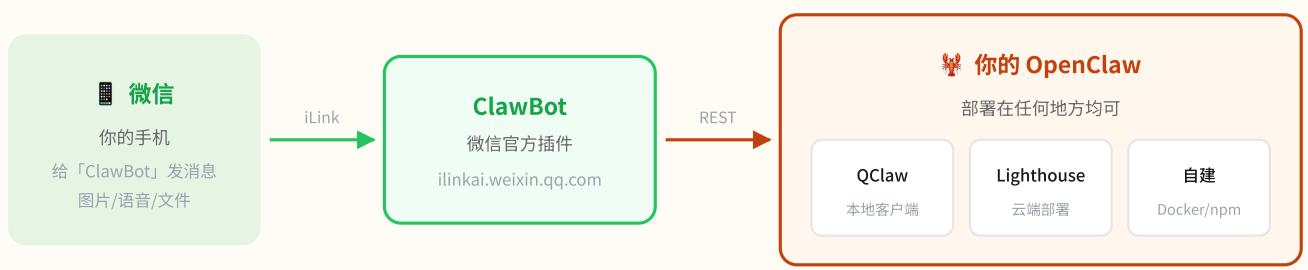
\includegraphics[keepaspectratio,alt={image}]{images/e9bef83d107967a1e26aa2964e8af2a7443fd5ab0cb4c2df64cd2499047e7acd.jpg}}

ClawBot是通道，不是龙虾本身--- 你的龙虾在哪里部署都行

\section{安装 ClawBot CLI}\label{ux5b89ux88c5-clawbot-cli}

在终端执行一条命令：

\begin{Shaded}
\begin{Highlighting}[]
\NormalTok{npx {-}y @tencent{-}weixin/openclaw{-}weixin{-}cli@latest install}
\end{Highlighting}
\end{Shaded}

npm 包在 @tencent-weixin 官方命名空间下，底层协议域名为
ilinkai.weixin.qq.com ，均为微信官方资产。

\section{2 扫码绑定}\label{ux626bux7801ux7ed1ux5b9a}

安装完成后扫码绑定微信即可。支持图片、语音、视频、文件等多种消息类型，群聊原生支持（
group\_id 字段）。

\section{三个注意事项}\label{ux4e09ux4e2aux6ce8ux610fux4e8bux9879}

iOS优先：需要微信8.0.70及以上版本，目前iOS已支持，安卓尚未确认时间表

灰度中：插件仍在逐步放量，不是所有用户都能看到入口（我 设置
插件）。没看到也别急，不代表不能用------直接跑安装命令试试

不是万能的：ClawBot定位是消息通道，不涉及微信自动化操作，不能获取聊天记录。腾讯保留对可连接的第三方AI服务类型进行限制的权利

{\def\LTcaptype{none} % do not increment counter
\begin{longtable}[]{@{}|l|l|l|@{}}
\toprule\noalign{}
\endhead
\bottomrule\noalign{}
\endlastfoot
\hline
维度 & ClawBot（官方） & 旧方案（iPad协议等） \\
\hline
合法性 & 微信官方产品，有法律条款 & 灰色地带，违反微信ToS \\
\hline
传输协议 & HTTP/JSON REST API（iLink协议） &
私有二进制协议（逆向工程） \\
\hline
稳定性 & 服务端维护，长期可靠 & 微信更新即可能失效 \\
\hline
封号风险 & 无 & 始终存在 \\
\hline
接入门槛 & 一条命令+扫码 & 需企业微信注册/开放平台权限申请 \\
\hline
\end{longtable}
}

\section{核心建议}\label{ux6838ux5fc3ux5efaux8bae-10}

ClawBot上线后，之前的企微中转、iPad协议等方案基本可以退役了。如果你已经在用旧方案，建议尽快迁移到ClawBot------官方通道不用担心封号，维护成本也低得多。

\section{微信旧方案 ClawBot
出现前的替代路径}\label{ux5faeux4fe1ux65e7ux65b9ux6848-clawbot-ux51faux73b0ux524dux7684ux66ffux4ee3ux8defux5f84}

以下三种方案是ClawBot上线之前的主流选择。ClawBot灰度完成后这些方案的必要性会大幅降低，但作为参考仍有价值。

\section{方案A：企业微信中转}\label{ux65b9ux6848aux4f01ux4e1aux5faeux4fe1ux4e2dux8f6c}

通过企业微信接入OpenClaw，再用微信插件打通企业微信和个人微信。合法合规，在微信生态内，需要企业微信管理后台权限。

\section{\texorpdfstring{方案 B：iPad 协议 \(^ +\)
中转网关}{方案 B：iPad 协议 \^{} + 中转网关}}\label{ux65b9ux6848-bipad-ux534fux8bae-ux4e2dux8f6cux7f51ux5173}

不走Web协议（高风险封号），走iPad协议。稳定性更高但技术门槛也更高。社区项目：

freestylefly/openclaw-wechat 、 laolin5564/openclaw-wechat 。

\section{方案C：微信小程序}\label{ux65b9ux6848cux5faeux4fe1ux5c0fux7a0bux5e8f}

2026 年新方案，通过小程序对接
OpenClaw。阿里云/腾讯云有预置镜像，降低部署门槛。

\section{注意}\label{ux6ce8ux610f-9}

旧方案需要持续维护，协议更新可能导致不可用。如果ClawBot已对你开放，强烈建议切换到官方通道。

\section{openclaw-china 统一插件
⼀站式国内平台⽀持}\label{openclaw-china-ux7edfux4e00ux63d2ux4ef6-ux7ad9ux5f0fux56fdux5185ux5e73ux53f0ux6301}

BytePioneer-AI/openclaw-china提供一站式国内平台支持，覆盖飞书、钉钉、QQ、企业微信、微信五个平台。

\begin{Shaded}
\begin{Highlighting}[]
\NormalTok{git clone https://github.com/BytePioneer{-}AI/openclaw{-}china.git  }
\NormalTok{cd openclaw{-}china  }
\NormalTok{pnpm install \&\& pnpm build  }
\NormalTok{openclaw china setup \# 交互式配置向导}
\end{Highlighting}
\end{Shaded}

特色功能包括：交互式配置向导减少手动配置、企业微信MP4视频播放器和多文件类型发送、腾讯云ASR语音转文字、钉钉日志增强（userId/groupId定位问题）。

选择建议：如果只用一个国内平台，直接安装对应的独立插件更轻量。如果要同时接入多个国内平台，openclaw-china
统一包更省事。

\section{18 远程访问}\label{ux8fdcux7a0bux8bbfux95ee}

OpenClaw Gateway 默认监听本地 ws: /127.0.0.1:18789
。当你需要从外部网络访问时，有以下几种方案。

\section{Tailscale Serve / Funnel
推荐⽅案}\label{tailscale-serve-funnel-ux63a8ux8350ux6848}

Tailscale 是 OpenClaw 官方推荐的远程访问方案，提供两种模式：

{\def\LTcaptype{none} % do not increment counter
\begin{longtable}[]{@{}|l|l|l|@{}}
\toprule\noalign{}
\endhead
\bottomrule\noalign{}
\endlastfoot
\hline
模式 & 访问范围 & 使用场景 \\
\hline
Serve & Tailscale 网络内的设备 & 自己的手机/平板访问家里的 OpenClaw \\
\hline
Funnel & 公网任何人 & 给 webhook 回调提供公网 URL（如飞书、Slack HTTP
模式） \\
\hline
\multicolumn{3}{@{}l@{}}{%
\# Serve: 仅 Tailscale 网络可访问} \\
\hline
\multicolumn{3}{@{}l@{}}{%
tailscale serve -\/-bg https+insecure://127.0.0.1:18789} \\
\hline
\multicolumn{3}{@{}l@{}}{%
\# Funnel: 公网可访问（用于 webhook 回调）} \\
\hline
\multicolumn{3}{@{}l@{}}{%
tailscale funnel -\/-bg https+insecure://127.0.0.1:18789} \\
\hline
\end{longtable}
}

\section{核心建议}\label{ux6838ux5fc3ux5efaux8bae-11}

大部分 channel（Telegram long-polling、Discord、Slack Socket Mode、钉钉
Stream 模式）都是 bot
主动连接服务器，不需要公网IP。只有需要webhook回调的场景（BlueBubbles、SlackHTTP模式）才需要Funnel暴露公网地址。

\section{SSH端口转发
最通⽤的⽅案}\label{sshux7aefux53e3ux8f6cux53d1-ux6700ux901aux7684ux6848}

如果 OpenClaw 运行在远程服务器上，用 SSH 隧道将 Gateway 端口转发到本地：

\begin{Shaded}
\begin{Highlighting}[]
\NormalTok{将远程服务器的18789端口转发到本地  }
\NormalTok{ssh {-}L 18789:127.0.0.1:18789 user@your{-}server  }
\NormalTok{\#后台运行  }
\NormalTok{ssh {-}fNL 18789:127.0.0.1:18789 user@your{-}server}
\end{Highlighting}
\end{Shaded}

转发后，本地客户端连接 ws: /127.0.0.1:18789 即可访问远程 Gateway。

\section{Dashboard Web UI（v2026.3.12
全面升级）}\label{dashboard-web-uiv2026.3.12-ux5168ux9762ux5347ux7ea7}

v2026.3.12推出了Dashboardv2，控制台从功能型界面升级为完整的模块化管理中心：

{\def\LTcaptype{none} % do not increment counter
\begin{longtable}[]{@{}|l|l|@{}}
\toprule\noalign{}
\endhead
\bottomrule\noalign{}
\endlastfoot
\hline
视图 & 功能 \\
\hline
Overview & Agent状态总览、Token用量、渠道连接状况 \\
\hline
Chat & 斜杠命令、消息搜索、导出、置顶消息 \\
\hline
Config & 模型配置、渠道开关、Plugin管理 \\
\hline
Agent & 记忆查看、Cron任务管理 \\
\hline
Session & 多会话管理、历史记录 \\
\hline
\multicolumn{2}{@{}l@{}}{%
\# Gateway 启动后默认可访问 \# 浏览器打开 http://127.0.0.1:18789
openclaw gateway -\/-port 18789 -\/-verbose} \\
\hline
\end{longtable}
}

新增命令面板（CommandPalette），按⌘K快速跳转。移动端新增底部标签栏，代替原来的悬浮按钮。

安全提醒：v2026.3.7 起 Gateway 认证要求显式设置 gateway.auth.mode
（token 或 password）。v2026.3.12 设备配对改用 Ephemeral
Token，连接更安全。不要在公网暴露未认证的 Gateway。

\section{Chrome 浏览器接入 v2026.3.13 新增 · 5-10
分钟}\label{chrome-ux6d4fux89c8ux5668ux63a5ux5165-v2026.3.13-ux65b0ux589e-5-10-ux5206ux949f}

v2026.3.13新增了最特别的一种「渠道」：直接附着到你正在使用的Chrome浏览器。Agent可以操控你已经登录的账号和页面------不需要另起账号，不需要APIKey，直接接管你的浏览器会话。

相比之前的浏览器工具（无头模式），这个方案的核心优势是：利用现有登录状态。Agent不需要再去登录各种网站，直接用你已经登录的状态操作。

\section{安装 Browser Relay
扩展}\label{ux5b89ux88c5-browser-relay-ux6269ux5c55}

在 Chrome 网上应用店安装 OpenClaw Browser Relay 扩展（扩展 ID：

nglingapjinhecnfejdcpihlpneeadjp ）。

\section{2 启动带调试端口的
Chrome}\label{ux542fux52a8ux5e26ux8c03ux8bd5ux7aefux53e3ux7684-chrome}

关闭所有Chrome窗口后，通过以下方式重新启动：

\begin{Shaded}
\begin{Highlighting}[]
\NormalTok{macOS   }
\NormalTok{open {-}a "Google Chrome" {-}{-}args {-}{-}remote{-}debugging{-}port=9222   }
\NormalTok{\#Windows   }
\NormalTok{"C:\textbackslash{}Program Files\textbackslash{}Google\textbackslash{}ChromeApplicationchrome.exe" {-}{-}remote{-}debugging{-}port=9222}
\end{Highlighting}
\end{Shaded}

或者在 openclaw.yaml 中使用内置 Profile 快捷方式：

\begin{Shaded}
\begin{Highlighting}[]
\NormalTok{browser: profile:"user" \#使用用户默认Profile \#profile:"chrome{-}relay" \#使用中继模式}
\end{Highlighting}
\end{Shaded}

\section{3 在 OpenClaw
中启用浏览器渠道}\label{ux5728-openclaw-ux4e2dux542fux7528ux6d4fux89c8ux5668ux6e20ux9053}

在 openclaw.yaml 中启用浏览器工具：

\begin{Shaded}
\begin{Highlighting}[]
\NormalTok{tools: browser: enabled: true attachMode:"devtools" \#v3.13新增，附着到已有会话}
\end{Highlighting}
\end{Shaded}

\section{4
向Agent下达浏览器任务}\label{ux5411agentux4e0bux8fbeux6d4fux89c8ux5668ux4efbux52a1}

重启Gateway后，直接给Agent发送浏览器相关指令，例如：「帮我整理浏览器里所有打开的GitHubPR」「把这个表单填写完」「截图保存当前页面」。

\section{核心建议}\label{ux6838ux5fc3ux5efaux8bae-12}

v2026.3.13 还支持 browser act
batching：把多个浏览器操作打包成批次执行，减少来回通信，自动化操作更稳定，不容易因为页面渲染时机问题卡住。

\section{注意}\label{ux6ce8ux610f-10}

ChromeDevTools附着模式意味着Agent可以读取你浏览器中所有页面的内容，包括已登录账号的私人信息。仅在信任的Agent配置下使用，不要在公共电脑或不受控的服务器上启用此功能。

\section{macOS
菜单栏伴侣应用}\label{macos-ux83dcux5355ux680fux4f34ux4fa3ux5e94ux7528}

OpenClaw 提供 macOS 原生客户端（ apps/macos/
），以菜单栏常驻应用的形式运行。功能包括：

一键启动/停止 Gateway

查看当前连接的 channel 状态

快速访问 Dashboard Web UI

系统通知（新消息、配对请求等）

iOS 和 Android 客户端也在开发中（ apps/ios/ 、 apps/android/
），代码已在主仓库中。

\section{核心建议}\label{ux6838ux5fc3ux5efaux8bae-13}

如果你同时使用多台设备，推荐 Tailscale Serve \(^ +\) macOS
菜单栏应用的组合：Mac 运行 Gateway
和菜单栏应用，手机/平板通过Tailscale网络访问。

\section{19 Skills工作原理}\label{skillsux5de5ux4f5cux539fux7406}

Skills是OpenClaw的能力扩展单元。理解它的加载机制，才能真正用好这个系统。

\section{三层优先级}\label{ux4e09ux5c42ux4f18ux5148ux7ea7}

OpenClaw的Skill有三个来源，按优先级从高到低排列：

{\def\LTcaptype{none} % do not increment counter
\begin{longtable}[]{@{}|l|l|l|@{}}
\toprule\noalign{}
\endhead
\bottomrule\noalign{}
\endlastfoot
\hline
优先级 & 位置 & 说明 \\
\hline
最高 & \textless workspace\textgreater/skills/ &
项目级Skills，只对当前工作区生效。适合针对特定项目定制的能力。 \\
\hline
中 & \textasciitilde/.openclaw/skills/ &
用户级Skills，全局生效。通过ClawHub安装或手动放置的Skills都在这里。 \\
\hline
最低 & bundled skills &
内置的55个Skills，随OpenClaw版本发布。不需要安装，开箱即用。 \\
\hline
\end{longtable}
}

\section{核心建议}\label{ux6838ux5fc3ux5efaux8bae-14}

如果同名Skill存在于多个层级，高优先级会覆盖低优先级。这意味着你可以在workspace级别「重写」一个内置Skill的行为，而不影响其他项目。

\section{Skill加载过程}\label{skillux52a0ux8f7dux8fc7ux7a0b}

当OpenClaw启动或收到消息时，Skills的加载遵循以下流程：

\section{读取Skill元数据}\label{ux8bfbux53d6skillux5143ux6570ux636e}

扫描三层目录，读取每个Skill的 SKILL.md
文件，解析名称、描述、触发条件、所需环境变量等元信息。

\section{2 应用环境变量}\label{ux5e94ux7528ux73afux5883ux53d8ux91cf}

如果Skill声明了需要的API Key或环境变量（如 GITHUB\_TOKEN ），系统会从
openclaw.json 的 env 字段中注入。缺少必要变量的Skill会被静默跳过。

\section{3 构建System Prompt}\label{ux6784ux5efasystem-prompt}

将所有可用Skills的描述注入到system
prompt中，告知模型当前可以调用哪些能力。这是模型「知道自己能做什么」的关键步骤。

\section{4 运行后恢复}\label{ux8fd0ux884cux540eux6062ux590d}

Skill执行完毕后，恢复原始环境变量和上下文状态，避免Skill之间互相干扰。

\section{ClawHub注册表}\label{clawhubux6ce8ux518cux8868}

ClawHub（ clawhub.com
）是OpenClaw的官方Skill注册表，类似npm之于Node.js。它提供：

公共Skills的发布和版本管理

基于向量搜索的Skill发现

下载量统计和社区评分

VirusTotal合作的安全扫描（但覆盖率有限）

\section{20
ClawHub与技能生态}\label{clawhubux4e0eux6280ux80fdux751fux6001}

13,729个技能只是冰山一角。加上Skills.sh的8.7万和SkillsMP的40万+，Agent技能生态正在爆发。

\section{市场概况}\label{ux5e02ux573aux6982ux51b5}

{\def\LTcaptype{none} % do not increment counter
\begin{longtable}[]{@{}|l|l|@{}}
\toprule\noalign{}
\endhead
\bottomrule\noalign{}
\endlastfoot
\hline
指标 & 数据 \\
\hline
总注册技能 & 13,729 \\
\hline
精选技能(awesome列表筛选) & 5,494 \\
\hline
被过滤技能（垃圾/重复/恶意） & 6,940 \\
\hline
被标记为恶意的 & 800+（约20\%在高峰期） \\
\hline
\end{longtable}
}

\section{注意}\label{ux6ce8ux610f-11}

ClawHub的质量问题非常严重。社区项目 awesome-openclaw-skills（31.4K
Stars）从13,729个技能中只精选了5,494个，剩下的大部分是垃圾、重复或低质量内容。安装任何第三方Skill前，务必查看源码。

\section{安装与搜索}\label{ux5b89ux88c5ux4e0eux641cux7d22}

\begin{Shaded}
\begin{Highlighting}[]
\NormalTok{\# 安装Skill  }
\NormalTok{openclaw skills install \textless{}skill{-}name\textgreater{}  }
\NormalTok{\# 搜索Skill  }
\NormalTok{openclaw skills search "browser automation"  }
\NormalTok{\# 列出已安装的Skills  }
\NormalTok{openclaw skills list  }
\NormalTok{\# 卸载Skill  }
\NormalTok{openclaw skills uninstall \textless{}skill{-}name\textgreater{}}
\end{Highlighting}
\end{Shaded}

ClawHub支持向量搜索，也就是说你可以用自然语言描述需求来搜索Skill，不必精确匹配名称。

技能分类Top 10

{\def\LTcaptype{none} % do not increment counter
\begin{longtable}[]{@{}|l|l|l|l|@{}}
\toprule\noalign{}
\endhead
\bottomrule\noalign{}
\endlastfoot
\hline
排名 & 分类 & 数量 & 说明 \\
\hline
1 & 编码Agent与IDE & 1,222 & 代码生成、调试、重构等开发辅助 \\
\hline
2 & Web与前端开发 & 938 & HTML/CSS/JS生成、组件开发 \\
\hline
3 & DevOps与云 & 408 & Docker、K8s、CI/CD管理 \\
\hline
4 & 搜索与研究 & 350 & 联网搜索、信息汇总 \\
\hline
5 & 浏览器与自动化 & 335 & 网页操作、表单填写、截图 \\
\hline
6 & 生产力与任务 & 206 & 日程、待办、项目管理 \\
\hline
7 & AI与LLM & 197 & 提示工程、模型切换、多Agent协作 \\
\hline
8 & CLI工具 & 186 & 终端命令增强、系统管理 \\
\hline
9 & Git与GitHub & 170 & 仓库管理、PR审查、Issue处理 \\
\hline
10 & 图片与视频生成 & 169 & AI绘图、视频处理 \\
\hline
\end{longtable}
}

编码相关的技能占了绝大多数（前两名合计2,160个），反映出OpenClaw用户中开发者占比极高。但也意味着这两个分类里重复和低质量Skill最多。

\section{第三方技能平台}\label{ux7b2cux4e09ux65b9ux6280ux80fdux5e73ux53f0}

ClawHub不是唯一的选择。2026年初，多个第三方技能平台相继上线，形成了一个跨Agent的技能共享生态。

{\def\LTcaptype{none} % do not increment counter
\begin{longtable}[]{@{}|l|l|l|l|l|@{}}
\toprule\noalign{}
\endhead
\bottomrule\noalign{}
\endlastfoot
\hline
平台 & 技能数量 & 出品方 & 定位 & 支持的Agent \\
\hline
ClawHub & 13,729 & OpenClaw 官方 & 策展市场（App
Store式），有向量搜索和版本回滚 & 仅OpenClaw \\
\hline
Skills.sh & 87,918 & Vercel & 开放市场（npm式），体量最大，跨Agent兼容 &
Claude Code、Cursor、Copilot、Codex、OpenClaw等20+ \\
\hline
SkillsMP & 400,000+ & 社区 &
社区爬取GitHub的SKILL.md文件，数量最多但质量参差 & 通用 \\
\hline
SkillHub & 7,000+ & 社区 & 每个Skill有AI自动评分，质量控制更好 & 通用 \\
\hline
扣子Skills & 早期阶段 & 字节跳动 &
技能商店+付费变现，支持「一句话生成」技能 & 扣子Agent \\
\hline
\end{longtable}
}

\section{Skills.sh：Agent技能的npm}\label{skills.shagentux6280ux80fdux7684npm}

Vercel在2026年1月20日推出的Skills.sh是目前体量最大的跨平台技能市场。它的核心理念是：一个Skill应该能在任何Agent中运行，不绑定特定平台。

\begin{Shaded}
\begin{Highlighting}[]
\NormalTok{从Skills.sh安装技能（一行命令）  }
\NormalTok{npx skills add owner/repo{-}name}
\end{Highlighting}
\end{Shaded}

Skills本质上是结构化指令文件（SKILL.md），注入Agent的上下文窗口，提供特定领域的程序化知识。它坐在MCP之上：MCP解决「Agent怎么连工具」，Skills解决「Agent怎么用好工具」。

\section{MCP生态与Skills的融合}\label{mcpux751fux6001ux4e0eskillsux7684ux878dux5408}

MCP（Model Context
Protocol）已捐赠给Linux基金会，成为Agent工具连接的事实标准。截至2026年3月：

mcp.so收录 \(^ { 1 8 , 4 2 0 + }\) MCP Servers

Smithery托管3,300-7,300+ MCP Server

已出现skill-to-mcp桥接工具，两套生态正在融合

一个趋势正在形成：MCP负责「连接」（让Agent能调用外部工具），Skills负责「智慧」（教Agent如何高效使用工具）。两者互补而非竞争。

实用建议：如果你已经在用ClaudeCode或Cursor等编程工具，可以从Skills.sh安装技能来增强能力，这些技能和OpenClaw的ClawHub
Skills使用相同的SKILL.md格式。跨平台复用是未来的大趋势。

\section{21 热门Skills推荐}\label{ux70edux95e8skillsux63a8ux8350}

55个内置技能开箱即用，加上社区精选的必装Top 10。

必装Top 10

{\def\LTcaptype{none} % do not increment counter
\begin{longtable}[]{@{}|l|l|l|l|@{}}
\toprule\noalign{}
\endhead
\bottomrule\noalign{}
\endlastfoot
\hline
排名 & Skill名称 & 下载量 & 用途 \\
\hline
1 & Gmail / Google & 32K+ & 邮件收发、日历管理、Google
Docs读写。基础设施级Skill，几乎所有用户都在用。 \\
\hline
2 & Agent Browser & 高 &
浏览器自动化：登录后台、填写表单、截图、导出PDF。基于Chrome DevTools
Protocol。 \\
\hline
3 & Summarize & 高 &
视频、网页、邮件内容的自动摘要。日常使用频率最高的Skill之一。 \\
\hline
4 & GitHub & 高 &
仓库管理、Issue处理、PR审查。技术用户标配，大幅减少网页操作时间。 \\
\hline
5 & Claude Code & 中 & 通过MCP协议桥接Claude
Code能力（Bash、Read、Write、Edit等），让OpenClaw获得专业编程能力。 \\
\hline
6 & Web Search & 高 &
联网搜索，让Agent能获取实时信息。支持多个搜索引擎后端。 \\
\hline
7 & File Manager & 中 &
本地文件的读写、移动、重命名等操作。需要注意安全权限。 \\
\hline
8 & Calendar & 中 & 日程查看与管理，支持Google
Calendar等多个日历服务。 \\
\hline
9 & Translator & 中 & 多语言翻译。对跨语言交流场景非常实用。 \\
\hline
10 & Image Gen & 中 & AI图片生成，集成DALL-E、Stable
Diffusion等后端。 \\
\hline
\end{longtable}
}

\section{内置55个技能分类一览}\label{ux5185ux7f6e55ux4e2aux6280ux80fdux5206ux7c7bux4e00ux89c8}

\section{通讯与社交}\label{ux901aux8bafux4e0eux793eux4ea4}

discord slack imsg （iMessage） bluebubbles wacli （WhatsApp CLI）
voice-call

\section{笔记与知识管理}\label{ux7b14ux8bb0ux4e0eux77e5ux8bc6ux7ba1ux7406}

obsidian notion apple-notes bear-notes trello things-mac apple-reminders

\section{开发工具}\label{ux5f00ux53d1ux5de5ux5177}

coding-agent github gh-issues tmux

\section{媒体处理}\label{ux5a92ux4f53ux5904ux7406}

spotify-player songsee sonoscli video-frames openai-image-gen gifgrep
camsnap

\section{AI与模型}\label{aiux4e0eux6a21ux578b}

gemini openai-whisper openai-whisper-api sherpa-onnx-tts model-usage

\section{搜索与浏览}\label{ux641cux7d22ux4e0eux6d4fux89c8}

xurl summarize blogwatcher gog （Google搜索） goplaces

\section{系统工具}\label{ux7cfbux7edfux5de5ux5177}

1password healthcheck session-logs himalaya （邮件CLI） peekaboo oracle
canvas

\section{智能家居}\label{ux667aux80fdux5bb6ux5c45}

openhue （Philips Hue灯光控制）

\section{生态工具}\label{ux751fux6001ux5de5ux5177}

clawhub （技能商店客户端） skill-creator （技能创建器） mcporter
（MCP桥接）

实用建议：不要一次性安装太多Skills。每个Skill都会增加systemprompt的长度，占用上下文窗口。建议从Top10中选择你真正需要的3-5个开始，用熟了再逐步扩展。

\section{22 自建Skill指南}\label{ux81eaux5efaskillux6307ux5357}

一个Skill的最小单位就是一个目录加一个 SKILL.md 文件。

\section{目录结构}\label{ux76eeux5f55ux7ed3ux6784-1}

\begin{Shaded}
\begin{Highlighting}[]
\NormalTok{my{-}skill/ SKILL.md \# 必须。Skill的核心定义文件 :—— scripts/\# 可选。辅助脚本 | —— helper.py templates/\# 可选。模板文件 | —— report.md —— README.md \# 可选。说明文档}
\end{Highlighting}
\end{Shaded}

唯一必须的文件是 SKILL.md
，其他都是可选的。最简单的Skill只需要一个SKILL.md就能工作。

\section{SKILL.md格式示例}\label{skill.mdux683cux5f0fux793aux4f8b}

\begin{Shaded}
\begin{Highlighting}[]
\NormalTok{My Custom Skill  }
\NormalTok{\# Description  }
\NormalTok{帮助用户进行每日工作汇总，生成结构化的日报。  }
\NormalTok{\# Trigger  }
\NormalTok{当用户提到「日报」「工作总结」「今日汇报」时激活。  }
\NormalTok{\# Instructions  }
\NormalTok{1. 询问用户今天完成了哪些工作  }
\NormalTok{2. 按项目分类整理  }
\NormalTok{3. 标注每项工作的状态（已完成/进行中/阻塞）  }
\NormalTok{4. 生成markdown格式的日报  }
\NormalTok{5. 保存到\textasciitilde{}/reports/YYYY{-}MM{-}DD.md  }
\NormalTok{\# Environment Variables  }
\NormalTok{{-} REPORTS\_DIR: 日报存储目录（默认\textasciitilde{}/reports)  }
\NormalTok{\# Tools Required  }
\NormalTok{{-} file\_write  }
\NormalTok{{-} memory\_search}
\end{Highlighting}
\end{Shaded}

\section{安装方式}\label{ux5b89ux88c5ux65b9ux5f0f}

{\def\LTcaptype{none} % do not increment counter
\begin{longtable}[]{@{}|l|l|l|l|@{}}
\toprule\noalign{}
\endhead
\bottomrule\noalign{}
\endlastfoot
\hline
方式 & 位置 & 生效范围 & 命令 \\
\hline
项目级 & & 仅当前工作区 & 直接将文件夹放到workspace的skills目录下 \\
\hline
全局 & & 所有会话 & 直接复制，或通过ClawHub安装 \\
\hline
\end{longtable}
}

\section{核心建议}\label{ux6838ux5fc3ux5efaux8bae-15}

项目级Skill非常适合团队协作场景：把Skill放进Git仓库的 skills/
目录，团队成员克隆仓库后就自动获得了相同的Agent能力。

\section{分享到ClawHub}\label{ux5206ux4eabux5230clawhub}

\section{准备Skill}\label{ux51c6ux5907skill}

确保SKILL.md格式正确，包含清晰的Description和Instructions。

\section{2 登录ClawHub}\label{ux767bux5f55clawhub}

\begin{Shaded}
\begin{Highlighting}[]
\NormalTok{openclaw clawhub login}
\end{Highlighting}
\end{Shaded}

\section{3 发布}\label{ux53d1ux5e03}

\begin{Shaded}
\begin{Highlighting}[]
\NormalTok{openclaw clawhub publish ./my{-}skill}
\end{Highlighting}
\end{Shaded}

发布后其他用户可以通过 openclaw skills install your-skill-name
安装。ClawHub会自动进行基础安全扫描，但不保证完全可靠（见下一节）。

\section{23 Skills安全}\label{skillsux5b89ux5168}

ClawHavoc供应链攻击是OpenClaw历史上最严重的安全事件之一。每个「养虾人」都应该了解。

\section{ClawHavoc供应链攻击}\label{clawhavocux4f9bux5e94ux94feux653bux51fb}

2026年1月底到2月初，OpenClaw社区遭遇了一场大规模供应链攻击，被安全研究机构KoiSecurity命名为「ClawHavoc」。

时间线

{\def\LTcaptype{none} % do not increment counter
\begin{longtable}[]{@{}|l|l|@{}}
\toprule\noalign{}
\endhead
\bottomrule\noalign{}
\endlastfoot
\hline
日期 & 事件 \\
\hline
1月27日 & 首个恶意Skill出现在ClawHub上，伪装成专业工具 \\
\hline
1月28-30日 &
攻击者快速上传大量恶意Skill，利用ClawHub缺乏审查机制的漏洞 \\
\hline
1月31日 & 攻击全面爆发，多名用户报告异常行为 \\
\hline
2月1日 & Koi Security正式命名该攻击为「ClawHavoc」 \\
\hline
2月上旬 & 社区展开大规模审计和清理 \\
\hline
\end{longtable}
}

攻击规模

{\def\LTcaptype{none} % do not increment counter
\begin{longtable}[]{@{}|l|l|@{}}
\toprule\noalign{}
\endhead
\bottomrule\noalign{}
\endlastfoot
\hline
指标 & 数据 \\
\hline
当时ClawHub技能总数 & 约2,857个 \\
\hline
初步确认恶意Skills & 341个（约12\%） \\
\hline
后续扫描发现的恶意Skills & 800+（约20\%） \\
\hline
可追溯到同一协调行动的 & 335个 \\
\hline
受影响设备 & 135,000+ \\
\hline
\end{longtable}
}

\section{注意}\label{ux6ce8ux610f-12}

ClawHub当时约 \(2 0 \%\)
的Skills被确认为恶意。这意味着如果你随机安装5个Skill，大概率至少有1个是恶意的。

\section{攻击手法}\label{ux653bux51fbux624bux6cd5}

攻击者的手法相当精密：

上传看似专业的Skill，名称和描述都很正常（如「advanced-code-review」「smart-scheduler」）

诱导用户安装后，Skill会建议安装一个「helper agent」来增强功能

实际植入的是 Atomic macOS Stealer（AMOS）信息窃取木马

更危险的是：攻击专门针对OpenClaw的持久记忆文件（ SOUL.md 和 MEMORY.md
），篡改Agent的长期行为指令

篡改SOUL.md意味着你的Agent被「洗脑」了。它的核心行为准则被改写，可能在后续所有交互中执行恶意操作，而你完全不知情。

\section{安全建议}\label{ux5b89ux5168ux5efaux8bae}

\section{1
安装前审查源码}\label{ux5b89ux88c5ux524dux5ba1ux67e5ux6e90ux7801}

永远不要盲目安装ClawHub上的Skill。去GitHub查看源码，确认SKILL.md中没有可疑的指令。特别注意任何要求额外安装「helper」或「agent」的内容。

\section{2 使用SecureClaw扫描}\label{ux4f7fux7528secureclawux626bux63cf}

社区推出了开源安全工具SecureClaw，可以扫描已安装的Skills检查恶意内容。虽然不能
\(1 0 0 \%\) 防护，但能拦住已知的攻击模式。

\begin{Shaded}
\begin{Highlighting}[]
\NormalTok{安装SecureClaw  }
\NormalTok{npm install {-}g secureclaw  }
\NormalTok{\# 扫描已安装的skills  }
\NormalTok{secureclaw scan \textasciitilde{}/.openclaw/skills/}
\end{Highlighting}
\end{Shaded}

\section{3
优先使用精选列表}\label{ux4f18ux5148ux4f7fux7528ux7cbeux9009ux5217ux8868}

参考 awesome-openclaw-skills 项目（31.4K
Stars）的精选列表，而不是直接在ClawHub上随意搜索。精选列表已经过滤掉了大量垃圾和恶意Skill。

\section{定期检查SOUL.md和MEMORY.md}\label{ux5b9aux671fux68c0ux67e5soul.mdux548cmemory.md}

养成习惯，定期检查这两个文件有没有被异常修改。如果发现不认识的内容，立即回滚并排查所有已安装的Skill。

\section{\texorpdfstring{2026年3月：VirusTotal审计发现 \(100 +\)
恶意Skills}{2026年3月：VirusTotal审计发现 100 + 恶意Skills}}\label{ux5e743ux6708virustotalux5ba1ux8ba1ux53d1ux73b0-100-ux6076ux610fskills}

VirusTotal对ClawHub进行了安全审计，发现超过100个Skills包含恶意代码，类型包括加密货币窃取、反向Shell后门和凭证窃取。这些恶意Skill并非来自ClawHavoc时期的残留，而是持续新增的。这说明ClawHub

的安全审核机制仍然不够完善，安装第三方 Skill 的风险并未随着时间降低。

\section{注意}\label{ux6ce8ux610f-13}

安全红线：拒绝任何要求你「下载 zip 文件」「执行 shell
脚本」「输入密码」的 Skill。这些是恶意 Skill 最常见的行为模式。

关键认知：OpenClaw的Skill本质上是受信任代码。一旦安装，它就拥有和你的OpenClaw实例相同的权限。没有沙箱隔离，没有权限分级。这和npm生态早期面临的问题一模一样，但后果可能更严重，因为OpenClaw可以访问你的邮件、日历、消息和文件系统。

\section{24
模型提供商总览}\label{ux6a21ux578bux63d0ux4f9bux5546ux603bux89c8}

OpenClaw支持十余家模型提供商，从国际顶尖到国产平价再到完全免费的本地模型，覆盖所有预算和场景。

OpenClaw最大的优势之一是模型自由：你不被绑定在某一家厂商上。通过
\textasciitilde/.openclaw/openclaw.json
配置文件，可以灵活切换主力模型、设置Fallback备选链、甚至让不同任务走不同模型。

支持的模型提供商一览

{\def\LTcaptype{none} % do not increment counter
\begin{longtable}[]{@{}|l|l|l|l|l|l|@{}}
\toprule\noalign{}
\endhead
\bottomrule\noalign{}
\endlastfoot
\hline
提供商 & 代表模型 & 输入价格 /1M tokens & 输出价格 /1M tokens & 接入方式
& 推荐场景 \\
\hline
Anthropic & Claude Sonnet 4.6 & \$3.00 & \$15.00 & 内置Provider &
Agent任务效果最佳 \\
\hline
OpenAI & GPT-5.4 & \$2.50 & \$15.00 & 内置Provider & 通用能力强 \\
\hline
Google & Gemini 3 Pro & \$2.00 & \$12.00 & 内置Provider &
多模态、超长上下文 \\
\hline
DeepSeek & DeepSeek-V3.2.2 / V4 & \$0.14 & \$0.28 & 自定义Provider &
极致低价、代码任务 \\
\hline
智谱GLM & GLM-5 & \$0.80 & \$2.56 & 内置（zai） & 国产最强代码能力 \\
\hline
智谱GLM & GLM-5-Turbo & \$0.96 & \$3.20 & 内置（zai） &
新首个专为OpenClaw训练优化的模型 \\
\hline
通义千问 & Qwen 3.5 Max & \$1.20 & \$6.00 & 插件（OAuth） &
中文NLP、代码生成 \\
\hline
豆包 & Seed 2.0 Pro & \$0.47 & \$2.37 & 自定义Provider &
批量处理、低成本 \\
\hline
百度文心 & 文心 5.0 & \textasciitilde\$0.58 & \textasciitilde\$1.16 &
自定义（需适配） & 百度云生态用户 \\
\hline
Kimi & Kimi K2.5 & \$0.60 & \$3.00 & 自定义Provider &
中文Agent、长上下文 \\
\hline
MiniMax & MiniMax M2.5 & \$0.50 & \$2.00 & 自定义Provider &
SWE-bench高分、性价比 \\
\hline
Ollama & Qwen3.5-Coder:32B & 免费 & 免费 & 自动发现 &
隐私敏感、零成本 \\
\hline
LM Studio & Devstral-24B & 免费 & 免费 & 自定义Provider &
本地GUI、模型测试 \\
\hline
\end{longtable}
}

\section{配置核心概念}\label{ux914dux7f6eux6838ux5fc3ux6982ux5ff5}

理解三个关键概念，就能掌握OpenClaw的模型配置：

内置Provider：Anthropic、OpenAI、Google、智谱（zai）等无需额外配置，设置API
Key即可使用

自定义Provider：DeepSeek、豆包、Kimi等需要在 models.providers 中手动添加

Fallback机制：主模型不可用时自动切换到备选，这是最核心的省钱策略

\begin{Shaded}
\begin{Highlighting}[]
\NormalTok{\{}\DataTypeTok{env}\OperatorTok{:}\NormalTok{ \{ }\StringTok{"API\_KEY\_NAME"}\OperatorTok{:} \StringTok{"sk{-}xxx"}\NormalTok{ \}}\OperatorTok{,}\DataTypeTok{agents}\OperatorTok{:}\NormalTok{ \{ }\DataTypeTok{defaults}\OperatorTok{:}\NormalTok{ \{}\DataTypeTok{model}\OperatorTok{:}\NormalTok{ \{}\DataTypeTok{primary}\OperatorTok{:} \StringTok{"provider/model{-}name"}\OperatorTok{,} \CommentTok{//主力模型fallbacks: ["provider/model{-}b"] //备选（主模型限速时自动切换)}\RegionMarkerTok{\}\}\}}\CommentTok{\},models:\{mode:"merge",//保留内置provider，叠加自定义providers:\{/\textbackslash{}*自定义provider配置\textbackslash{}*/\}1}
\end{Highlighting}
\end{Shaded}

\section{核心建议}\label{ux6838ux5fc3ux5efaux8bae-16}

设置 models.mode: ``merge''
非常重要。它能保留所有内置Provider的同时叠加你的自定义配置。如果不设置，自定义配置会覆盖内置Provider。

\section{25 国际模型配置}\label{ux56fdux9645ux6a21ux578bux914dux7f6e}

Anthropic Claude、OpenAI GPT、Google Gemini的完整配置指南。

\section{Anthropic Claude}\label{anthropic-claude}

Claude是OpenClaw的默认模型提供商，也是社区公认的Agent任务效果最好的模型。Sonnet4.6在工具调用的准确率和稳定性上显著领先其他模型。

{\def\LTcaptype{none} % do not increment counter
\begin{longtable}[]{@{}|l|l|l|l|l|@{}}
\toprule\noalign{}
\endhead
\bottomrule\noalign{}
\endlastfoot
\hline
模型 & 输入/1M & 输出/1M & 上下文 & 定位 \\
\hline
Claude Opus 4.6 & \$5.00 & \$25.00 & 200K & 最强推理，复杂任务 \\
\hline
Claude Sonnet 4.6 & \$3.00 & \$15.00 & 200K & 主力模型，性价比之选 \\
\hline
Claude Haiku 4.5 & \$1.00 & \$5.00 & 200K & 轻量任务，高速低成本 \\
\hline
\end{longtable}
}

\section{配置方式}\label{ux914dux7f6eux65b9ux5f0f}

Claude是内置Provider，配置最简单：

\section{环境变量方式}\label{ux73afux5883ux53d8ux91cfux65b9ux5f0f}

ANTHROPIC\_API\_KEY \(\equiv\) sk-ant-xxx\\
\# 或在 openclaw.json 中设置\\
\{env: \{``ANTHROPIC\_API\_KEY'': ``sk-ant-xxx''\}\}

模型ID： anthropic/claude-opus-4-6 、 anthropic/claude-sonnet-4-6 、
anthropic/claude-haiku-4-5

\section{注意}\label{ux6ce8ux610f-14}

Anthropic已封杀OAuth认证方式。使用Claude
Pro/Max订阅账户通过OAuth连接OpenClaw的用户会收到警告甚至被锁定账户。目前唯一合法路径是使用APIKey（按量付费）。

\section{省钱技巧：}\label{ux7701ux94b1ux6280ux5de7}

Batch API可享 \(5 0 \%\) 折扣（输入输出均半价）

Prompt Caching可降低重复上下文成本达 \(9 0 \%\)

OpenAI GPT

{\def\LTcaptype{none} % do not increment counter
\begin{longtable}[]{@{}|l|l|l|l|l|@{}}
\toprule\noalign{}
\endhead
\bottomrule\noalign{}
\endlastfoot
\hline
模型 & 输入/1M & 输出/1M & 上下文 & 定位 \\
\hline
GPT-5.4 & \$2.50 & \$15.00 & 272K（标准） & 最新旗舰 \\
\hline
GPT-5.4 (\textgreater272K) & \$5.00 & \$15.00 & 1.05M & 超长上下文 \\
\hline
GPT-5.2 & \$1.75 & \$14.00 & --- & 上一代旗舰 \\
\hline
GPT-5 & \$1.25 & \$10.00 & --- & 性价比之选 \\
\hline
\end{longtable}
}

\section{配置方式}\label{ux914dux7f6eux65b9ux5f0f-1}

OPENAI\_API\_KEY \(\equiv\) sk-xxxx

\section{注意}\label{ux6ce8ux610f-15}

GPT-5.4超过272K上下文后输入价格翻倍（ \(\langle \$ 2.50\to 55.00\)
）。如果你的Agent会话上下文较长，注意控制长度或设置消费限额。

Google Gemini

{\def\LTcaptype{none} % do not increment counter
\begin{longtable}[]{@{}|l|l|l|l|l|@{}}
\toprule\noalign{}
\endhead
\bottomrule\noalign{}
\endlastfoot
\hline
模型 & 输入/1M & 输出/1M & 上下文 & 定位 \\
\hline
Gemini 3 Pro (≤200K) & \$2.00 & \$12.00 & 200K & 旗舰多模态 \\
\hline
Gemini 3 Pro (\textgreater200K) & \$4.00 & \$18.00 & 2M & 超长上下文 \\
\hline
Gemini 3 Flash & \$0.50 & \$3.00 & --- & 高速低成本 \\
\hline
\end{longtable}
}

\section{配置方式}\label{ux914dux7f6eux65b9ux5f0f-2}

GOOGLE\_API\_KEY \(\equiv\) xxx\#或通过GoogleAIStudio免费额度使用

Gemini的独家优势是2M上下文窗口和慷慨的免费额度（Flash每日有免费请求）。多模态能力也是三家中最强的。

\section{核心建议}\label{ux6838ux5fc3ux5efaux8bae-17}

GeminiFlash的免费额度非常适合用作心跳（Heartbeat）和定时任务（Cron）的模型，这些场景不需要最强能力但需要持续运行，用免费模型可以把成本降到零。

\section{26 国产模型配置}\label{ux56fdux4ea7ux6a21ux578bux914dux7f6e}

国产模型是OpenClaw用户省钱的核心武器。DeepSeek-V3.2.2的输入价格仅为Claude
Sonnet的1/20。

\section{DeepSeek}\label{deepseek}

性价比之王。DeepSeek-V3.2.2是当前稳定版（2025年12月发布），输入价格仅\$0.14/M
tokens，是目前OpenClaw社区最常用的低成本模型。

{\def\LTcaptype{none} % do not increment counter
\begin{longtable}[]{@{}|l|l|l|l|@{}}
\toprule\noalign{}
\endhead
\bottomrule\noalign{}
\endlastfoot
\hline
模型 & 输入/1M & 输出/1M & 定位 \\
\hline
DeepSeek-V3.2.2 (deepseek-chat) & \$0.14 & \$0.28 &
当前稳定版，极致低价 \\
\hline
DeepSeek-R1 (deepseek-reasoner) & \$0.55\textasciitilde0.70 &
\$2.19\textasciitilde2.50 & 深度推理 \\
\hline
\end{longtable}
}

\section{配置方式（自定义Provider）}\label{ux914dux7f6eux65b9ux5f0fux81eaux5b9aux4e49provider}

\begin{Shaded}
\begin{Highlighting}[]
\NormalTok{\{}\DataTypeTok{env}\OperatorTok{:}\NormalTok{ \{ }\StringTok{"DEEPSEEK\_API\_KEY"}\OperatorTok{:} \StringTok{"sk{-}xxx"}\NormalTok{ \}}\OperatorTok{,}\DataTypeTok{models}\OperatorTok{:}\NormalTok{ \{}\DataTypeTok{mode}\OperatorTok{:} \StringTok{"merge"}\OperatorTok{,}\DataTypeTok{providers}\OperatorTok{:}\NormalTok{ \{}\DataTypeTok{deepseek}\OperatorTok{:}\NormalTok{ \{}\DataTypeTok{baseUrl}\OperatorTok{:} \StringTok{"https://api deepseek.com/v1"}\OperatorTok{,} \DataTypeTok{apiKey}\OperatorTok{:} \StringTok{"$\{}\SpecialCharTok{\textbackslash{}D}\StringTok{EEPSEEK\_API\_KEY\}"} \OperatorTok{,}\DataTypeTok{api}\OperatorTok{:} \StringTok{"openai{-}completions"}\OperatorTok{,}\DataTypeTok{models}\OperatorTok{:}\NormalTok{ [}\DataTypeTok{id}\OperatorTok{:}\StringTok{"deepseek{-}chat"}\OperatorTok{,}\DataTypeTok{contextWindow}\OperatorTok{:} \DecValTok{128000}\OperatorTok{,}\DataTypeTok{maxTokens}\OperatorTok{:} \DecValTok{8192}\NormalTok{ ]}\OperatorTok{,}\DataTypeTok{id}\OperatorTok{:}\StringTok{"deepseek{-}reasoner"}\OperatorTok{,}\DataTypeTok{contextWindow}\OperatorTok{:} \DecValTok{128000}\OperatorTok{,}\DataTypeTok{maxTokens}\OperatorTok{:} \DecValTok{8192}\NormalTok{ ]\} \}}
\end{Highlighting}
\end{Shaded}

\section{注意}\label{ux6ce8ux610f-16}

DeepSeek高峰期偶有延迟甚至不可用，不建议作为唯一Provider。务必搭配Fallback模型兜底。

\section{智谱GLM}\label{ux667aux8c31glm}

国产模型中代码能力最强的选择。GLM-5在SWE-bench上拿到了开源模型最高分，价格仅\$0.80/M输入。更妙的是，OpenClaw内置了zai
Provider，配置极为简单。

{\def\LTcaptype{none} % do not increment counter
\begin{longtable}[]{@{}|l|l|l|l|@{}}
\toprule\noalign{}
\endhead
\bottomrule\noalign{}
\endlastfoot
\hline
模型 & 输入/1M & 输出/1M & 定位 \\
\hline
GLM-5-Turbo & \$0.96 & \$3.20 & NEW首个专为OpenClaw优化的基座模型 \\
\hline
GLM-5 & \$0.80 & \$2.56 & 旗舰，代码能力强 \\
\hline
GLM-4.5 & \$0.60 & \$2.20 & 上一代主力 \\
\hline
GLM-4.7-Flash & 免费 & 免费 & 轻量免费 \\
\hline
GLM-4.5-Flash & 免费 & 免费 & 轻量免费 \\
\hline
\end{longtable}
}

\section{??GLM-5-Turbo：第一个「龙虾模型」}\label{glm-5-turboux7b2cux4e00ux4e2aux9f99ux867eux6a21ux578b}

2026年3月16日，智谱发布GLM-5-Turbo，官方定位是「首个龙虾模型」------历史上第一个从训练阶段就专为OpenClaw使用场景深度优化的基座模型。和普通大模型接入OpenClaw不同，GLM-5-Turbo在训练时就针对了四个OpenClaw核心能力：

工具调用（ToolCalling）：更准确的工具选择和参数传递

指令跟踪（Command Following）：多步骤任务不丢失上下文

持久任务（Persistent Tasks）：长时间运行不降级

长链执行（Long-chain Execution）：减少中途失败和幻觉

{\def\LTcaptype{none} % do not increment counter
\begin{longtable}[]{@{}|l|l|@{}}
\toprule\noalign{}
\endhead
\bottomrule\noalign{}
\endlastfoot
\hline
参数 & GLM-5-Turbo \\
\hline
最大输出 Token & 128K \\
\hline
上下文长度 & 200K \\
\hline
支持功能 & 思考模式 · 函数调用 · 流式输出 · 上下文缓存 · MCP \\
\hline
当前状态 & 已上线，闭源（已接入 OpenRouter / Coze / 美团 / Trae） \\
\hline
API 定价 & 输入 \$0.96/M · 输出 \$3.20/M（比 GLM-5 贵 20\%） \\
\hline
龙虾套餐 & 体验月卡 ¥39 (3500万 tokens) · 进阶月卡 ¥99 (1亿 tokens) \\
\hline
\end{longtable}
}

\section{配置方式}\label{ux914dux7f6eux65b9ux5f0f-3}

\begin{Shaded}
\begin{Highlighting}[]
\NormalTok{GLM{-}5{-}Turbo（已上线，API直接可用）  }
\NormalTok{\{env: \{ "ZAI\_API\_KEY": "sk{-}xxx" \},agents: \{ defaults: \{model: \{primary: "zai/glm{-}5{-}turbo" \}\}\}  }
\NormalTok{\}  }
\NormalTok{\# GLM{-}5（正式版，推荐）  }
\NormalTok{\{env: \{ "ZAI\_API\_KEY": "sk{-}xxx" \},agents: \{defaults: \{model: \{primary: "zai/glm{-}5" \}\}\}  }
\NormalTok{\}}
\end{Highlighting}
\end{Shaded}

CLI 快速配置： openclaw onboard -auth-choice zai-api-key 。注意 z.ai *
和 z-ai * 前缀会自动转换为 zai * 。

\section{核心建议}\label{ux6838ux5fc3ux5efaux8bae-18}

GLMFlash系列完全免费，适合心跳任务和简单对话。GLM-5-Turbo已上线并接入多个平台（OpenRouter/Coze
/ 美团 / Trae），「龙虾套餐」月卡 ¥39 起，是国内 OpenClaw
用户的新选择。注意 GLM-5-Turbo 比 GLM-5 贵 \(2 0 \%\)
，如果你的Agent任务不重度依赖工具调用和长链执行，GLM-5仍然是性价比更高的选择。

\section{通义千问 Qwen}\label{ux901aux4e49ux5343ux95ee-qwen}

Qwen3.5是阿里2026年2月发布的最新版本（397B总参数/17B激活，MoE架构，已开源）。代码专用的Qwen3.5-Coder性价比极高。

{\def\LTcaptype{none} % do not increment counter
\begin{longtable}[]{@{}|l|l|l|l|@{}}
\toprule\noalign{}
\endhead
\bottomrule\noalign{}
\endlastfoot
\hline
模型 & 输入/1M & 输出/1M & 定位 \\
\hline
Qwen 3.5 Max & \$1.20 & \$6.00 & 旗舰模型（397B-A17B） \\
\hline
Qwen 3.5 Plus & \$0.40 & \$1.20 & 主力平衡 \\
\hline
Qwen 3.5Coder & \$0.22 & \$1.00 & 代码专用，性价比极高 \\
\hline
Qwen 3.5 8B & \$0.05 & \$0.40 & 轻量低成本 \\
\hline
\end{longtable}
}

配置方式（插件 \(^ +\) OAuth）

\begin{Shaded}
\begin{Highlighting}[]
\NormalTok{通过插件接入，OAuth设备码认证（无需API Key）  }
\NormalTok{openclaw plugins enable qwen{-}portal{-}auth  }
\NormalTok{openclaw gateway restart  }
\NormalTok{openclaw models auth login {-}{-}provider qwen{-}portal {-}{-}set{-}default}
\end{Highlighting}
\end{Shaded}

模型ID： qwen-portal/coder-model 、 qwen-portal/vision-model
。每日2,000次免费请求。

\section{豆包 Doubao}\label{ux8c46ux5305-doubao}

{\def\LTcaptype{none} % do not increment counter
\begin{longtable}[]{@{}|l|l|l|l|@{}}
\toprule\noalign{}
\endhead
\bottomrule\noalign{}
\endlastfoot
\hline
模型 & 输入/1M & 输出/1M & 定位 \\
\hline
Seed 2.0 Pro & \$0.47 & \$2.37 & 旗舰推理，对标GPT-5.2 \\
\hline
Doubao 1.5 Pro-32k & \$0.11 & --- & 通用对话，极致低价 \\
\hline
Doubao 1.5 Lite-32k & \$0.042 & --- & 最便宜的选择之一 \\
\hline
\end{longtable}
}

\section{配置方式（自定义Provider）}\label{ux914dux7f6eux65b9ux5f0fux81eaux5b9aux4e49provider-1}

\begin{Shaded}
\begin{Highlighting}[]
\NormalTok{\{}\DataTypeTok{env}\OperatorTok{:}\NormalTok{ \{ }\StringTok{"DOUBAO\_API\_KEY"}\OperatorTok{:} \StringTok{"xxx"}\NormalTok{ \}}\OperatorTok{,}\DataTypeTok{models}\OperatorTok{:}\NormalTok{ \{}\DataTypeTok{mode}\OperatorTok{:} \StringTok{"merge"}\OperatorTok{,}\DataTypeTok{providers}\OperatorTok{:}\NormalTok{ \{}\DataTypeTok{doubao}\OperatorTok{:}\NormalTok{ \{}\DataTypeTok{baseUrl}\OperatorTok{:} \StringTok{"https://ark.cn{-}beijing.volces.com/api/v3"}\OperatorTok{,}\DataTypeTok{apiKey}\OperatorTok{:} \StringTok{"$}\SpecialCharTok{\textbackslash{}\{\textbackslash{}t}\StringTok{ext\{DOUBAO\_API\_KEY\}}\SpecialCharTok{\textbackslash{}\}}\StringTok{ "}\OperatorTok{,}\DataTypeTok{api}\OperatorTok{:} \StringTok{"openai{-}completions"}\OperatorTok{,}\DataTypeTok{models}\OperatorTok{:}\NormalTok{ [}\DataTypeTok{id}\OperatorTok{:} \StringTok{"doubao{-}seed{-}2.0{-}pro"}\OperatorTok{,}\DataTypeTok{contextWindow}\OperatorTok{:} \DecValTok{128000}\OperatorTok{,}\DataTypeTok{maxTokens}\OperatorTok{:} \DecValTok{4096}\NormalTok{ ] \} \} \} \}}
\end{Highlighting}
\end{Shaded}

\section{Kimi（月之暗面）}\label{kimiux6708ux4e4bux6697ux9762}

{\def\LTcaptype{none} % do not increment counter
\begin{longtable}[]{@{}|l|l|l|l|@{}}
\toprule\noalign{}
\endhead
\bottomrule\noalign{}
\endlastfoot
\hline
模型 & 输入/1M & 输出/1M & 定位 \\
\hline
Kimi K2.5 & \$0.60 & \$3.00 & 最新旗舰 \\
\hline
Kimi K2 0905 & \$0.39 & \$1.90 & 性价比版 \\
\hline
\end{longtable}
}

\section{配置方式}\label{ux914dux7f6eux65b9ux5f0f-4}

\begin{Shaded}
\begin{Highlighting}[]
\NormalTok{\{}\DataTypeTok{env}\OperatorTok{:}\NormalTok{ \{}\StringTok{"MOONSHOT\_API\_KEY"}\OperatorTok{:} \StringTok{"sk{-}xxx"}\NormalTok{\}}\OperatorTok{,}\DataTypeTok{models}\OperatorTok{:}\NormalTok{ \{}\DataTypeTok{mode}\OperatorTok{:}\StringTok{"merge"}\OperatorTok{,}\DataTypeTok{providers}\OperatorTok{:}\NormalTok{\{}\DataTypeTok{moonshot}\OperatorTok{:}\NormalTok{\{}\DataTypeTok{baseUrl}\OperatorTok{:}\StringTok{"https://api.moonshot.cn/v1"}\OperatorTok{,} \DataTypeTok{apiKey}\OperatorTok{:}\StringTok{"$\{MOONSHOT\_API\_KEY\}"}\OperatorTok{,}\DataTypeTok{api}\OperatorTok{:}\StringTok{"openai{-}completions"}\OperatorTok{,}\DataTypeTok{models}\OperatorTok{:}\NormalTok{[}\DataTypeTok{id}\OperatorTok{:}\StringTok{"kimi{-}k2.5"}\OperatorTok{,}\DataTypeTok{contextWindow}\OperatorTok{:}\DecValTok{256000}\OperatorTok{,}\DataTypeTok{maxTokens}\OperatorTok{:}\DecValTok{8192}\NormalTok{]\}\}}\DecValTok{1}
\end{Highlighting}
\end{Shaded}

也可通过OpenRouter接入： openrouter/moonshotai/kimi-k2.5

\section{百度文心}\label{ux767eux5ea6ux6587ux5fc3}

文心5.0于2026年1月22日发布（2.4万亿参数，原生全模态，激活参数比
\({ < } 3 \%\) ）。

{\def\LTcaptype{none} % do not increment counter
\begin{longtable}[]{@{}|l|l|l|l|@{}}
\toprule\noalign{}
\endhead
\bottomrule\noalign{}
\endlastfoot
\hline
模型 & 输入价格 & 输出价格 & 定位 \\
\hline
文心5.0 & \textasciitilde\$0.58/M & \textasciitilde\$1.16/M &
最新旗舰（2.4万亿参数） \\
\hline
ERNIE Speed & 免费 & 免费 & 轻量 \\
\hline
ERNIE Lite & 免费 & 免费 & 最轻量 \\
\hline
\end{longtable}
}

\section{注意}\label{ux6ce8ux610f-17}

百度API格式与OpenAI不完全兼容，需要通过one-api等中转工具适配。在OpenClaw社区中存在感最低，配置复杂度最高。如果没有特别的百度云生态绑定，建议优先选择其他国产模型。

\section{MiniMax}\label{minimax}

MiniMax M2.5（230B参数）在SWE-Bench上得分 \(8 0 . 2 \%\)
，代码能力突出。

{\def\LTcaptype{none} % do not increment counter
\begin{longtable}[]{@{}|l|l|l|l|@{}}
\toprule\noalign{}
\endhead
\bottomrule\noalign{}
\endlastfoot
\hline
模型 & 输入/1M & 输出/1M & 定位 \\
\hline
MiniMax M2.5 & \$0.50 & \$2.00 & 旗舰，SWE-bench 80.2\% \\
\hline
\end{longtable}
}

\section{配置方式}\label{ux914dux7f6eux65b9ux5f0f-5}

\begin{Shaded}
\begin{Highlighting}[]
\KeywordTok{\{}\FunctionTok{env}\KeywordTok{:}\AttributeTok{ }\KeywordTok{\{}\AttributeTok{ }\FunctionTok{"MINIMAX\_API\_KEY"}\KeywordTok{:}\AttributeTok{ }\StringTok{"xxx"}\AttributeTok{ }\KeywordTok{\},}\FunctionTok{models}\KeywordTok{:}\AttributeTok{ }\KeywordTok{\{}\FunctionTok{mode}\KeywordTok{:}\AttributeTok{ }\StringTok{"merge"}\KeywordTok{,}\FunctionTok{providers}\KeywordTok{:}\AttributeTok{ }\KeywordTok{\{}\FunctionTok{minimax}\KeywordTok{:}\AttributeTok{ }\KeywordTok{\{}\FunctionTok{baseUrl}\KeywordTok{:}\AttributeTok{ }\StringTok{"https://api.minimax chat/v1"}\KeywordTok{,}\AttributeTok{ }\FunctionTok{apiKey}\KeywordTok{:}\AttributeTok{ }\StringTok{"$\{\textbackslash{}MINIMAX\_API\_KEY\}"}\AttributeTok{ }\KeywordTok{,}\FunctionTok{api}\KeywordTok{:}\AttributeTok{ }\StringTok{"openai{-}completions"}\KeywordTok{,}\FunctionTok{models}\KeywordTok{:}\AttributeTok{ }\KeywordTok{[}\AttributeTok{id:}\StringTok{"minimax{-}m2.5"}\KeywordTok{,}\FunctionTok{contextWindow}\KeywordTok{:}\AttributeTok{ }\DecValTok{128000}\KeywordTok{,}\FunctionTok{maxTokens}\KeywordTok{:}\AttributeTok{ }\DecValTok{8192}\AttributeTok{ }\KeywordTok{]\}}\DecValTok{1}
\end{Highlighting}
\end{Shaded}

\section{聚合平台：一个API
Key调多个模型}\label{ux805aux5408ux5e73ux53f0ux4e00ux4e2aapi-keyux8c03ux591aux4e2aux6a21ux578b}

\section{硅基流动
SiliconFlow（国内首选）}\label{ux7845ux57faux6d41ux52a8-siliconflowux56fdux5185ux9996ux9009}

国内最大的模型聚合平台，一个API调用多个开源模型，延迟低，有免费额度。

\begin{Shaded}
\begin{Highlighting}[]
\NormalTok{\{}\DataTypeTok{env}\OperatorTok{:}\NormalTok{ \{}\StringTok{"SILICONFLOW\_API\_KEY"}\OperatorTok{:} \StringTok{"sk{-}xxx"}\NormalTok{\}}\OperatorTok{,}\DataTypeTok{models}\OperatorTok{:}\NormalTok{ \{}\DataTypeTok{mode}\OperatorTok{:}\StringTok{"merge"}\OperatorTok{,}\DataTypeTok{providers}\OperatorTok{:}\NormalTok{\{}\DataTypeTok{siliconflow}\OperatorTok{:}\NormalTok{\{}\DataTypeTok{baseUrl}\OperatorTok{:}\StringTok{"https://api.siliconflow.cn/v1"}\OperatorTok{,} \DataTypeTok{apiKey}\OperatorTok{:}\StringTok{"$\{SILICONFLOW\_API\_KEY\}"}\OperatorTok{,}\DataTypeTok{api}\OperatorTok{:}\StringTok{"openai{-}completions"}\OperatorTok{,}\DataTypeTok{models}\OperatorTok{:}\NormalTok{[}\DataTypeTok{id}\OperatorTok{:}\StringTok{"Pro/deepseek{-}ai/DeepSeek{-}V3.2"}\OperatorTok{,}\DataTypeTok{contextWindow}\OperatorTok{:}\DecValTok{128000}\OperatorTok{,}\DataTypeTok{maxTokens}\OperatorTok{:}\DecValTok{8192}\NormalTok{\}}\OperatorTok{,}\NormalTok{\{}\DataTypeTok{id}\OperatorTok{:}\StringTok{"Pro/zai{-}org/GLM{-}5"}\OperatorTok{,}\DataTypeTok{contextWindow}\OperatorTok{:}\DecValTok{128000}\OperatorTok{,}\DataTypeTok{maxTokens}\OperatorTok{:}\DecValTok{8192}\NormalTok{\}]}\DecValTok{1}\NormalTok{\}}\DecValTok{1}\NormalTok{\}}\DecValTok{1}\NormalTok{\}}
\end{Highlighting}
\end{Shaded}

\section{OpenRouter（国际首选）}\label{openrouterux56fdux9645ux9996ux9009}

\({ 2 9 0 + }\) 模型，OpenClaw内置支持，但有 \(5 . 5 \%\) 平台费。

\begin{Shaded}
\begin{Highlighting}[]
\NormalTok{openclaw onboard {-}{-}auth{-}choice apiKey {-}{-}token{-}provider openrouter {-}{-}token "$OPENROUTER\_API\_KEY}
\NormalTok{// 模型ID格式: openrouter/provider/model}
\NormalTok{// openrouter/deepseek/deepseek{-}chat}
\NormalTok{// openrouter/openrouter/auto (自动选择最优模型)}
\end{Highlighting}
\end{Shaded}

\section{one-api /
new-api（自建方案）}\label{one-api-new-apiux81eaux5efaux65b9ux6848}

开源API管理工具，自建网关，统一管理多个APIKey，支持负载均衡和故障转移。适合团队使用。

\section{注意}\label{ux6ce8ux610f-18}

中转服务必须支持OpenAI的Responses API（ /v1/responses
路径），不仅仅是Chat Completions API。部分旧版中转工具不支持此接口。

\section{Coding Plan
包月套餐对比}\label{coding-plan-ux5305ux6708ux5957ux9910ux5bf9ux6bd4}

国内⼚商 AI 编程订阅

2026年，国内主要AI厂商和云平台纷纷推出了面向AI编程工具（OpenClaw、Cursor、Claude
Code等）的CodingPlan包月套餐。相比按量付费的API，包月套餐的优势是成本可预期、无需管理APIKey余额，尤其适合个人开发者和轻度到中度使用者。

厂商自营 Coding Plan

{\def\LTcaptype{none} % do not increment counter
\begin{longtable}[]{@{}lllll@{}}
\toprule\noalign{}
\endhead
\bottomrule\noalign{}
\endlastfoot
厂商 & 套餐档位 & 月费 & 模型 & 特色/限制 \\
\multirow{5}{*}{智谱GLM} & Lite & \textasciitilde49元 & GLM-4.7 &
MCP联网100次/月 \\
& Pro & \textasciitilde80元 & GLM-4.7 & 速度快40-60\%, MCP 1000次/月 \\
& Max & \textasciitilde160元 & GLM-4.7 + GLM-5 & 唯一含GLM-5, MCP
4000次/月 \\
& New 龙虾体验卡 & 39元 & GLM-5-Turbo & 3500万tokens/月,
OpenClaw专项优化 \\
& New 龙虾进阶卡 & 99元 & GLM-5-Turbo & 1亿tokens/月,
OpenClaw专项优化 \\
\multirow{3}{*}{Kimi} & Andante & 49元 & Kimi K2.5 & 基础档,
Token计量 \\
& Moderato & 99元 & Kimi K2.5 & 中档 \\
& Allegretto & 199元 & Kimi K2.5 & 每5小时100-500次请求 \\
\multirow{3}{*}{MiniMax} & Starter & 29元 & M2.5 & 无每周限额,
性价比最高 \\
& Standard & 49元 & M2.5 & 年付省17\% \\
& Premium & 119元 & M2.5 & 重度用户 \\
\end{longtable}
}

\section{云平台聚合 Coding
Plan}\label{ux4e91ux5e73ux53f0ux805aux5408-coding-plan}

云平台方案的最大优势是一个套餐包含多家模型，可自由切换。

{\def\LTcaptype{none} % do not increment counter
\begin{longtable}[]{@{}llllll@{}}
\toprule\noalign{}
\endhead
\bottomrule\noalign{}
\endlastfoot
平台 & 档位 & 原价/月 & 首月优惠 & 包含模型 & 用量 \\
\multirow{2}{*}{阿里云百炼} & Lite & 40元 & 7.9元 & Qwen + GLM + Kimi +
MiniMax & \textasciitilde18,000次/月 \\
& Pro & 200元 & 39.9元 & 同上 & \textasciitilde90,000次/月 \\
\multirow{2}{*}{腾讯云} & Lite & 40元 & 7.9元 & 混元2.0 + GLM-5 + Kimi
K2.5 + M2.5 & 每5h \textasciitilde1,200次 \\
& Pro & 200元 & 39.9元 & 同上 & 每5h \textasciitilde6,000次 \\
\multirow{2}{*}{火山引擎} & Lite & 40元 & 8.91元 & 豆包Code + GLM-4.7 +
DeepSeek-V3.2.2 + Kimi & 每5h \textasciitilde1,200次 \\
& Pro & 200元 & 44.91元 & 同上 & 每5h \textasciitilde6,000次 \\
\end{longtable}
}

\section{Coding Plan
选型建议}\label{coding-plan-ux9009ux578bux5efaux8bae}

\section{核心建议}\label{ux6838ux5fc3ux5efaux8bae-19}

首月体验（7.9元起）：阿里云百炼或腾讯云 Lite
档，首月仅7.9元，包含4家模型自由切换，是零风险的入门方式。

长期性价比：MiniMaxStarter（29元/月）无每周限额，M2.5代码能力强；如果需要多模型切换，云平台续费5折（约20元/月）也很划算。

追求最强单模型：智谱Max（160元/月）是目前唯一包含GLM-5的自营套餐；腾讯云也新增了GLM-5支持。

重度用户：CodingPlan普遍有频率限制（每5小时N次），如果你需要高频调用，建议直接使用API按量付费，搭配Fallback链控制成本。

\section{注意}\label{ux6ce8ux610f-19}

注意Coding Plan的限制：智谱2026年2月已涨价 \(3 0 \%\)
并取消首购优惠，有周限制机制；Kimi仅限个人使用、禁止企业开发；大部分云平台套餐次月续费为5折而非原价。购买前务必确认续费价格。

\section{27
本地模型与推荐方案}\label{ux672cux5730ux6a21ux578bux4e0eux63a8ux8350ux65b9ux6848}

完全免费，完全离线，完全隐私。代价是需要硬件投入，能力上限受限。

\section{Ollama}\label{ollama}

最流行的本地模型运行方案，完全免费，OpenClaw能自动发现已安装的模型。

\begin{Shaded}
\begin{Highlighting}[]
\NormalTok{1. 安装Ollama后拉取模型  }
\NormalTok{ollama pull qwen2.5:32b  }
\NormalTok{ollama pull deepseek{-}r1:14b}
\end{Highlighting}
\end{Shaded}

\begin{Shaded}
\begin{Highlighting}[]
\NormalTok{2. 设置环境变量（任意值即可）  }
\NormalTok{ollama\_API\_KEY=ollama{-}local}
\end{Highlighting}
\end{Shaded}

\begin{Shaded}
\begin{Highlighting}[]
\NormalTok{3. OpenClaw自动发现支持工具调用的本地模型}
\end{Highlighting}
\end{Shaded}

\section{注意}\label{ux6ce8ux610f-20}

不要使用 /v1 OpenAI兼容URL，会导致工具调用异常。让OpenClaw使用原生Ollama
API URL进行自动发现。冷启动有延迟，建议保持模型加载状态。

\section{LM Studio}\label{lm-studio}

有GUI界面的本地模型方案，使用Llama.cpp后端，原始性能更好。工具调用在流式模式下比Ollama更稳定。OpenClaw创始人Peter
Steinberger个人使用LM Studio作为本地后端。

\begin{Shaded}
\begin{Highlighting}[]
\NormalTok{\{ models: \{ mode:"merge", providers:\{ lmstudio:\{ baseUrl:"http://127.0.0.1:1234/v1", apiKey:"lm{-}studio", api:"openai{-}responses", models:[ \{ id:"model{-}name",contextWindow:32768,maxTokens:8192\} ] \} \} \}}
\end{Highlighting}
\end{Shaded}

\section{推荐本地模型}\label{ux63a8ux8350ux672cux5730ux6a21ux578b}

{\def\LTcaptype{none} % do not increment counter
\begin{longtable}[]{@{}|l|l|l|l|@{}}
\toprule\noalign{}
\endhead
\bottomrule\noalign{}
\endlastfoot
\hline
模型 & 参数量 & 推荐场景 & 最低内存 \\
\hline
Qwen3.5-Coder:32B & 32B & 代码生成、Agent任务 & 32GB RAM \\
\hline
Devstral-24B & 24B & Agent/工具调用 & 32GB RAM \\
\hline
Qwen 2.5:32B & 32B & 通用任务 & 32GB RAM \\
\hline
DeepSeek-R1:14B & 14B & 推理任务 & 16GB RAM \\
\hline
Llama 3.3 & 8B-70B & 通用任务 & 16-64GB RAM \\
\hline
\end{longtable}
}

硬件要求速查：运行3-7B参数模型最低需要16GB
RAM。运行32B参数模型推荐32GBRAM。如果有NVIDIA/Apple Silicon
GPU会显著加速推理。

\section{五套推荐方案}\label{ux4e94ux5957ux63a8ux8350ux65b9ux6848}

\section{\texorpdfstring{方案一：极致省钱（月均 \({ < } \$ 5\)
）}{方案一：极致省钱（月均 \{ \textless{} \} \textbackslash\$ 5 ）}}\label{ux65b9ux6848ux4e00ux6781ux81f4ux7701ux94b1ux6708ux5747-5}

主力：DeepSeek-V3.2（\$0.14/\$0.28）

备选：Qwen 3.5 Plus（\$0.40/\$1.20）

心跳/Cron：GLM-4.5-Flash（免费）

推理任务：DeepSeek-R1（\$0.55/\$2.19）

适合：个人开发者、学习探索。风险：DeepSeek高峰期延迟，需Fallback兜底。

\section{方案二：国产性价比（月均\$5-15）}\label{ux65b9ux6848ux4e8cux56fdux4ea7ux6027ux4ef7ux6bd4ux6708ux57475-15}

主力：GLM-5（\$0.80/\$2.56）

备选：DeepSeek-V3.2（\$0.14/\$0.28）

推理增强：Kimi K2.5（\$0.60/\$3.00）

简单任务：GLM-4.5-Flash（免费）

适合：国内用户，追求中文体验和稳定性。GLM-5代码能力强，延迟低。

\section{方案三：国际平衡（月均\$10-30）}\label{ux65b9ux6848ux4e09ux56fdux9645ux5e73ux8861ux6708ux574710-30}

主力：Claude Sonnet 4.6（\$3.00/\$15.00）

轻量：Claude Haiku 4.5 或 Gemini Flash

复杂任务：Claude Opus 4.6（按需升级）

心跳/Cron：Gemini Flash（免费额度）

适合：追求Agent效果最优、预算充足。Claude在Agent/工具调用场景效果最好。

\section{方案四：混合最优（月均\$5-20，推荐）}\label{ux65b9ux6848ux56dbux6df7ux5408ux6700ux4f18ux6708ux57475-20ux63a8ux8350}

复杂任务：Claude Sonnet 4.6

日常对话：DeepSeek-V3.2

心跳/定时：Gemini Flash 或本地 Ollama

Fallback链：Sonnet Haiku DeepSeek-V3.2

大多数用户的最佳选择。兼顾效果和成本，Fallback机制自动处理限速。

\begin{Shaded}
\begin{Highlighting}[]
\NormalTok{// 方案四的Fallback配置示例  }
\NormalTok{\{  }
\NormalTok{agents: \{  }
\NormalTok{    defaults: \{  }
\NormalTok{        model: \{  }
\NormalTok{            primary: "anthropic/claude{-}sonnet{-}4{-}6",  }
\NormalTok{            fallbacks: [  }
\NormalTok{                "anthropic/claude{-}haiku{-}4{-}5",  }
\NormalTok{                "deepseek/deepseek{-}chat"  }
\NormalTok{            ]  }
\NormalTok{        \}  }
\NormalTok{    \}  }
\NormalTok{\}}
\end{Highlighting}
\end{Shaded}

\section{方案五：完全免费}\label{ux65b9ux6848ux4e94ux5b8cux5168ux514dux8d39}

选项A：本地 Ollama \(^ +\) Qwen3.5-Coder:32B 或 Devstral-24B（需32GB
RAM）

选项B：免费API组合 --- GLM-4.5-Flash \(^ +\) ERNIE Speed \(^ +\) Gemini
Flash

适合：隐私敏感、纯实验用途。本地方案需要较好的硬件。

价格速查排行（输入价格 /1M tokens）

{\def\LTcaptype{none} % do not increment counter
\begin{longtable}[]{@{}|l|l|l|l|l|@{}}
\toprule\noalign{}
\endhead
\bottomrule\noalign{}
\endlastfoot
\hline
\# & 模型 & 输入 & 输出 & 一句话评价 \\
\hline
- & Ollama / LM Studio & 免费 & 免费 & 仅消耗本地算力 \\
\hline
- & GLM Flash / ERNIE Speed & 免费 & 免费 & 云端免费tier \\
\hline
1 & Doubao 1.5 Lite-32k & \$0.042 & - & 最便宜云端对话 \\
\hline
2 & Qwen3 8B & \$0.05 & \$0.40 & 轻量低成本 \\
\hline
3 & DeepSeek-V3.2 & \$0.14 & \$0.28 & 性价比之王 \\
\hline
4 & Qwen3 Coder 480B & \$0.22 & \$1.00 & 代码专用性价比 \\
\hline
5 & Qwen 3.5 Plus & \$0.40 & \$1.20 & 平衡之选 \\
\hline
6 & Doubao Seed 2.0 Pro & \$0.47 & \$2.37 & 国产旗舰 \\
\hline
7 & Gemini 3 Flash & \$0.50 & \$3.00 & 国际低价 \\
\hline
8 & Kimi K2.5 & \$0.60 & \$3.00 & 中文旗舰 \\
\hline
- & GLM-5-Turbo & \$0.96 & \$3.20 & 首个OpenClaw专项优化模型 \\
\hline
9 & GLM-5 & \$0.80 & \$2.56 & 国产代码最强 \\
\hline
10 & Claude Haiku 4.5 & \$1.00 & \$5.00 & 国际轻量 \\
\hline
11 & Gemini 3 Pro & \$2.00 & \$12.00 & Google旗舰 \\
\hline
12 & GPT-5.4 & \$2.50 & \$15.00 & OpenAI旗舰 \\
\hline
13 & Claude Sonnet 4.6 & \$3.00 & \$15.00 & Agent效果最佳 \\
\hline
14 & Claude Opus 4.6 & \$5.00 & \$25.00 & 最强也最贵 \\
\hline
\end{longtable}
}

配置要点速查

{\def\LTcaptype{none} % do not increment counter
\begin{longtable}[]{@{}|l|l|@{}}
\toprule\noalign{}
\endhead
\bottomrule\noalign{}
\endlastfoot
\hline
操作 & 命令/配置 \\
\hline
引导式配置 & openclaw onboard \\
\hline
查看已配置模型 & openclaw models list \\
\hline
测试连通性 & openclaw models status -\/-probe \\
\hline
设置主力模型 & openclaw config set agentsDefaults.modelprimary
provider/model \\
\hline
添加Fallback & 编辑 openclaw.json 的 fallbacks 数组 \\
\hline
重启网关 & openclaw gateway restart (改配置后必须执行) \\
\hline
环境变量引用 & 配置中用 "\$VAR\_NAME" 引用env中的变量 \\
\hline
\end{longtable}
}

\section{28 安全模型}\label{ux5b89ux5168ux6a21ux578b}

OpenClaw的安全模型建立在「默认不信任」的基础上，但创始人自己坦言：「prompt
injection没解决，有绝对风险。」

\section{默认不信任}\label{ux9ed8ux8ba4ux4e0dux4fe1ux4efb}

OpenClaw对所有入站消息的默认态度是：不可信。具体体现在以下几个机制：

\section{DM配对保护}\label{dmux914dux5bf9ux4fddux62a4}

当一个未知的用户通过任何消息渠道（WhatsApp、Telegram等）给你的OpenClaw发私信时，系统不会处理消息。取而代之的是返回一个配对码（pairingcode），只有在你手动批准后，该用户的消息才会被处理。这防止了陌生人滥用你的Agent（以及你的API额度）。

\section{群组沙箱模式}\label{ux7fa4ux7ec4ux6c99ux7bb1ux6a21ux5f0f}

在群组环境中，OpenClaw默认运行在沙箱模式：

每个群组的会话互相隔离

MEMORY.md （长期记忆）只在私聊的mainsession中加载，群组看不到

可以配置 requireMention ，只有@提及时才响应

\section{工具访问控制}\label{ux5de5ux5177ux8bbfux95eeux63a7ux5236}

{\def\LTcaptype{none} % do not increment counter
\begin{longtable}[]{@{}|l|l|@{}}
\toprule\noalign{}
\endhead
\bottomrule\noalign{}
\endlastfoot
\hline
配置项 & 作用 \\
\hline
allowlist & 白名单模式。只允许列出的工具被调用，其他一律禁止。 \\
\hline
denylist & 黑名单模式。禁止列出的工具，其他允许。 \\
\hline
browser开关 & 可完全禁用浏览器自动化能力 \\
\hline
canvas开关 & 可禁用Canvas可视化 \\
\hline
nodes开关 & 可禁用对本地设备节点的控制（如摄像头、录屏） \\
\hline
\end{longtable}
}

\section{v2026.3.8新增：ACP身份验证}\label{v2026.3.8ux65b0ux589eacpux8eabux4efdux9a8cux8bc1}

v2026.3.8 引入了 ACP Provenance（代理身份验证）功能，让 Agent
能验证「谁在跟它交互」，减少身份伪造攻击：

\begin{Shaded}
\begin{Highlighting}[]
\NormalTok{配置ACP身份验证级别  }
\NormalTok{openclaw acp {-}{-}provenance off \#关闭（默认）  }
\NormalTok{openclaw acp {-}{-}provenance meta \#注入来源元数据  }
\NormalTok{openclaw acp {-}{-}provenance meta+receipt \#元数据 + 可见回执}
\end{Highlighting}
\end{Shaded}

\section{v2026.3.7新增：Gateway认证要求}\label{v2026.3.7ux65b0ux589egatewayux8ba4ux8bc1ux8981ux6c42}

v2026.3.7 引入了一个Breaking Change：Gateway认证现在要求显式设置
gateway.auth.mode 。你必须明确选择 token 或 password
认证方式，不再有「无认证」的默认选项。

\begin{Shaded}
\begin{Highlighting}[]
\ErrorTok{在openclaw.json中配置}  
\FunctionTok{\{} \DataTypeTok{"gateway"}\FunctionTok{:} \FunctionTok{\{} \DataTypeTok{"auth"}\FunctionTok{:} \FunctionTok{\{} \DataTypeTok{"mode"}\FunctionTok{:} \StringTok{"token"}\FunctionTok{,} \ErrorTok{//或}\DataTypeTok{"password"} \DataTypeTok{"token"}\FunctionTok{:} \StringTok{"your{-}secret{-}token"} \FunctionTok{\}} \FunctionTok{\}} \FunctionTok{\}}
\end{Highlighting}
\end{Shaded}

\section{注意}\label{ux6ce8ux610f-21}

如果你从旧版本升级到v2026.3.7且没有配置认证，Gateway将拒绝启动。这是一个有意为之的设计，强制所有用户设置认证。

\section{v2026.3.11 + v2026.3.12
安全更新}\label{v2026.3.11-v2026.3.12-ux5b89ux5168ux66f4ux65b0}

2026年3月12-13日，两个版本接连发布，都包含重要安全改进：

\section{WebSocket
跨站劫持漏洞修复（v3.11）}\label{websocket-ux8de8ux7ad9ux52abux6301ux6f0fux6d1eux4feeux590dv3.11}

修复了Gateway/WebSocket浏览器来源校验漏洞------攻击者可以通过trusted-proxy路径绕过来源检查，实施跨站WebSocket劫持（CSWSH）。这是对早期ClawJacked漏洞类型的一个新变体，现已在v3.11中修复。

\section{注意}\label{ux6ce8ux610f-22}

如果你的Gateway通过反向代理（Nginx、Caddy等）对外提供服务，强烈建议升级到v2026.3.11或更高版本。

\section{设备配对 Ephemeral
Token（v3.12）}\label{ux8bbeux5907ux914dux5bf9-ephemeral-tokenv3.12}

设备配对流程改用短期bootstraptoken，不再在聊天消息或QR码扫描内容中嵌入长期Gateway凭证。这消除了一类攻击面：配对二维码或消息被截获后，攻击者无法用其长期访问你的
Gateway。

\section{禁用隐式 Workspace Plugin
自动加载（v3.12）}\label{ux7981ux7528ux9690ux5f0f-workspace-plugin-ux81eaux52a8ux52a0ux8f7dv3.12}

克隆仓库不再自动执行其中包含的 workspace plugin 代码。每个仓库的 plugin
首次加载时都需要显式信任确认。这解决了供应链攻击的一条途径：恶意仓库无法在你不知情的情况下执行插件代码。

\begin{Shaded}
\begin{Highlighting}[]
\NormalTok{\# 显式信任一个 workspace 的 plugin}
\NormalTok{openclaw workspace trust /path/to/repo}
\end{Highlighting}
\end{Shaded}

\section{Peter的坦诚}\label{peterux7684ux5766ux8bda}

OpenClaw创始人Peter
Steinberger在多个场合对安全问题保持了罕见的坦诚。他的原话：

「This is all vibe code. Prompt injection hasn't been solved. There are
absolute risks.」（这全是vibe code。Prompt
injection没有被解决。存在绝对风险。）

这种坦诚值得尊重，但也意味着：如果你要在生产环境中使用OpenClaw，安全防护必须由你自己负责。OpenClaw提供了基础的安全机制，但远谈不上「企业级安全」。

\section{29 已知安全事件}\label{ux5df2ux77e5ux5b89ux5168ux4e8bux4ef6}

在不到5个月的历史中，OpenClaw已经经历了至少9起重大安全事件，CNNVD累计收录漏洞82个（严重12个、高危21个），工信部级别的安全预警也已发出。

CVE-2026-25253：远程代码执行漏洞

{\def\LTcaptype{none} % do not increment counter
\begin{longtable}[]{@{}|l|l|@{}}
\toprule\noalign{}
\endhead
\bottomrule\noalign{}
\endlastfoot
\hline
项目 & 详情 \\
\hline
CVE编号 & CVE-2026-25253 \\
\hline
CVSS评分 & 8.8/10（高危） \\
\hline
类型 & 远程代码执行（RCE） \\
\hline
原理 & WebSocket origin header绕过。攻击者可以伪造origin
header连接到暴露的Gateway，在OpenClaw实例上执行任意代码。 \\
\hline
影响范围 & 所有暴露到公网且未配置认证的OpenClaw实例 \\
\hline
状态 & 已修复（v2026.3.2加固了WebSocket origin检查） \\
\hline
\end{longtable}
}

\section{注意}\label{ux6ce8ux610f-23}

这个漏洞的危害极大：攻击者可以远程在你的服务器上执行任何命令，包括读取文件、安装恶意软件、窃取APIKey等。如果你还在运行v2026.3.2之前的版本，请立即升级。

\section{ClawHavoc供应链攻击}\label{clawhavocux4f9bux5e94ux94feux653bux51fb-1}

详见本指南§23Skills安全。这是OpenClaw历史上影响最广的安全事件，135,000+设备受到影响，ClawHub约
\(2 0 \%\) 的Skills在高峰期被确认为恶意。

\section{Anthropic封杀OAuth}\label{anthropicux5c01ux6740oauth}

2026年1月，Anthropic官方封禁了Claude
Pro/Max订阅账户通过OAuth连接OpenClaw的能力。

许多用户收到账户警告或被直接锁定

部分用户的订阅被取消且无法恢复

目前唯一合法的连接方式：使用Anthropic API Key（按量付费）

这不算传统意义上的「安全事件」，但对大量用户造成了实质损失。如果你还在用OAuth方式连接Anthropic，请立即切换到APIKey方式。

\begin{Shaded}
\begin{Highlighting}[]
\NormalTok{正确的配置方式(APIKey)   }
\NormalTok{\{ "env": \{ "ANTHROPIC\_API\_KEY":"sk{-}ant{-}your{-}key{-}here" \}   }
\NormalTok{\}}
\end{Highlighting}
\end{Shaded}

\section{谷歌封号事件}\label{ux8c37ux6b4cux5c01ux53f7ux4e8bux4ef6}

2026年2月初，谷歌大规模封禁OpenClaw用户的Google账号。受影响的用户描述：

「每月花250美元使用Gemini API，被封却毫无预警」

封禁范围包括Gmail、Google Drive、Google Calendar等全部Google服务

部分用户的OpenClaw通过Gmail Skill大量调用Google API，触发了滥用检测

GitHub Issue \#14203记录了大量受影响用户的反馈

\section{核心建议}\label{ux6838ux5fc3ux5efaux8bae-20}

如果你的OpenClaw使用了Google相关Skill，建议：(1) 使用专门的Google
Workspace账号而非个人主账号；(2) 控制API调用频率，避免触发滥用检测；(3)
重要数据做好备份。

\section{30,000+台未认证暴露实例}\label{ux53f0ux672aux8ba4ux8bc1ux66b4ux9732ux5b9eux4f8b}

安全研究者通过互联网扫描发现，超过30,000台OpenClaw实例暴露在公网上且未配置任何认证。这些实例的Gateway端口（默认18789）对任何人开放，意味着：

任何人都可以连接并向你的Agent发送指令

你的API额度可能被消耗殆尽

你的个人数据（邮件、文件、消息记录）可能被读取

结合CVE-2026-25253，攻击者可以在你的服务器上执行任意代码

\section{注意}\label{ux6ce8ux610f-24}

如果你的OpenClaw部署在云服务器上，请立即检查：(1)
Gateway是否只绑定了localhost；(2) 防火墙是否开放了18789端口；(3)
是否配置了认证（v2026.3.7已强制要求）。

\section{工信部安全预警（2026年3月8-9日）}\label{ux5de5ux4fe1ux90e8ux5b89ux5168ux9884ux8b662026ux5e743ux67088-9ux65e5}

工信部和国家互联网应急中心（CNCERT）正式发布了OpenClaw安全风险预警。这是国内官方机构首次对一个开源AIAgent项目发出安全预警，说明其影响面已经非常大。

预警指出的主要风险：

默认或不当配置下极易引发网络攻击和信息泄露

OpenClaw的「模糊信任边界」 \(+\) 持续运行 \(+\) 自主决策 \(+\)
调用系统资源的特性，使其成为高价值攻击目标

建议加强权限控制、审计机制和安全加固

\section{360发现WebSocket
0Day漏洞（2026年3月22日）}\label{ux53d1ux73b0websocket-0dayux6f0fux6d1e2026ux5e743ux670822ux65e5}

360安全云团队发现了一个OpenClaw Gateway
WebSocket未认证升级漏洞（0Day），OpenClaw创始人Peter已回信确认。攻击者可通过WebSocket静默绕过认证，接管Agent网关，导致资源耗尽或系统全面崩溃。360已将该漏洞提交至CNVD，此事一度登上微博热搜第一。

这个漏洞与早期的CVE-2026-25253属于同一类攻击面（WebSocket认证），但利用路径不同。虽然v2026.3.7已强制Gateway认证，但部分配置场景下仍可被绕过。

\section{漏洞统计（截至2026年3月）}\label{ux6f0fux6d1eux7edfux8ba1ux622aux81f32026ux5e743ux6708}

截至3月11日，CNNVD（国家信息安全漏洞库）累计收录OpenClaw相关漏洞82个：

{\def\LTcaptype{none} % do not increment counter
\begin{longtable}[]{@{}|l|l|l|@{}}
\toprule\noalign{}
\endhead
\bottomrule\noalign{}
\endlastfoot
\hline
严重程度 & 数量 & 典型类型 \\
\hline
严重 & 12 & 远程代码执行、WebSocket劫持 \\
\hline
高危 & 21 & 路径穿越、沙箱逃逸、内存耗尽 \\
\hline
中危 & 47 & 白名单绕过、allow-always持久化、脚本注入 \\
\hline
低危 & 2 & 信息泄露 \\
\hline
\end{longtable}
}

\section{注意}\label{ux6ce8ux610f-25}

82个漏洞在5个月内被发现，说明OpenClaw的代码审计还远未完成。好消息是社区和安全公司在持续审计，坏消息是你永远不知道下一个0Day什么时候出现。保持版本更新是最基本的安全措施。

\section{恶意npm包伪装事件（2026年3月）}\label{ux6076ux610fnpmux5305ux4f2aux88c5ux4e8bux4ef62026ux5e743ux6708}

一个名为 @openclaw-ai/openclawai 的恶意 npm 包伪装成 OpenClaw
官方安装器，实际安装的是GhostLoaderRAT（远程访问木马），窃取用户凭证和加密钱包。该包已于3月10日从npm注册表移除。

\section{注意}\label{ux6ce8ux610f-26}

安装 OpenClaw 请务必使用官方命令（ npm install -g openclaw@latest
），不要搜索和安装来历不明的第三方包。认准包名 openclaw
，而非任何带前缀的变体。

\section{ClawJacked零点击漏洞（2026年3月初）}\label{clawjackedux96f6ux70b9ux51fbux6f0fux6d1e2026ux5e743ux6708ux521d}

安全公司 Oasis Security
发现了一个关键漏洞：恶意网站可以通过浏览器会话静默暴力破解本地 OpenClaw
实例，实现完全控制。这意味着你只要访问一个恶意网页，本地运行的OpenClaw就可能被接管。

\section{核心建议}\label{ux6838ux5fc3ux5efaux8bae-21}

防护建议：(1) 保持 OpenClaw 更新到最新版本；(2) 不要在运行 OpenClaw
的设备上访问不可信网站；(3) 配置 Gateway 认证。

\section{30 成本控制}\label{ux6210ux672cux63a7ux5236}

API费用是OpenClaw运营的最大成本。不做控制，真的会一觉醒来收到\$1,100的账单。

\section{为什么成本会失控}\label{ux4e3aux4ec0ux4e48ux6210ux672cux4f1aux5931ux63a7}

OpenClaw的Token消耗远超普通聊天场景。原因有几个：

每次Agent思考都是多轮推理：一个简单的任务可能触发5-10次API调用

Skills的描述会注入system prompt，增加每次请求的输入token

记忆系统（MEMORY.md \(^ +\) Daily Logs）会在每次请求中附带上下文

Agent 24/7运行，定时任务（cron）不断触发API调用

多轮思考 \(^ +\) 多工具调用的Token消耗可能是传统聊天的几十甚至上百倍

真实案例：社区中频繁出现的恐怖故事：用户设置了Agent处理邮件的cron任务，晚上睡觉前一切正常，第二天早上发现API账单暴涨到\$1,100。原因是Agent在处理邮件时进入了循环推理，整晚不停调用API。

\section{Token优化策略：Fallback链}\label{tokenux4f18ux5316ux7b56ux7565fallbackux94fe}

Fallback链是OpenClaw最核心的省钱策略。原理很简单：主模型不可用时自动降级到更便宜的模型。但更聪明的用法是主动利用它来控制成本。

\begin{Shaded}
\begin{Highlighting}[]
\NormalTok{\{ "agents": \{ " defaults": \{ "model": \{ "primary": "anthropic/claude{-}sonnet{-}4{-}6", "fallbacks": [ "anthropic/claude{-}haiku{-}4{-}5", "deepseek/deepseek{-}chat" ] \} \} \} \}}
\end{Highlighting}
\end{Shaded}

\section{不同方案的成本对比}\label{ux4e0dux540cux65b9ux6848ux7684ux6210ux672cux5bf9ux6bd4}

{\def\LTcaptype{none} % do not increment counter
\begin{longtable}[]{@{}|l|l|l|l|@{}}
\toprule\noalign{}
\endhead
\bottomrule\noalign{}
\endlastfoot
\hline
策略 & 主力模型 & 输入价格/百万token & 相对成本 \\
\hline
全用Claude Sonnet & Claude Sonnet 4.6 & \$3.00 & 100\%（基准） \\
\hline
Sonnet + Haiku Fallback & Sonnet → Haiku & \$3.00 / \$1.00 &
约50-60\% \\
\hline
Sonnet → Haiku → DeepSeek & 三级Fallback & \$3.00 / \$1.00 / \$0.14 &
约5-20\% \\
\hline
纯DeepSeek & DeepSeek-V3 & \$0.14 & 约5\% \\
\hline
本地Ollama & Qwen3-Coder等 & \$0 & 0\%（仅电费） \\
\hline
\end{longtable}
}

从Claude Sonnet切换到「Sonnet Haiku DeepSeek」三级Fallback链，可以降低
\(8 0 { - } 9 5 \%\)
的API成本。大部分简单任务（问候、查天气、简单查询）会自动走最便宜的模型，只有复杂任务才会用到主力模型。

\section{预算限制设置}\label{ux9884ux7b97ux9650ux5236ux8bbeux7f6e}

OpenClaw支持在配置中设置预算上限：

\begin{Shaded}
\begin{Highlighting}[]
\FunctionTok{\{}
    \DataTypeTok{"agents"}\FunctionTok{:} \FunctionTok{\{}
        \DataTypeTok{"defaults"}\FunctionTok{:} \FunctionTok{\{}
            \DataTypeTok{"budget"}\FunctionTok{:} \FunctionTok{\{}
                \DataTypeTok{"maxTokensPerDay"}\FunctionTok{:} \DecValTok{500000}\FunctionTok{,}
                \DataTypeTok{"maxCostPerDay"}\FunctionTok{:} \FloatTok{5.00}
            \FunctionTok{\}}
        \FunctionTok{\}}
    \FunctionTok{\}}
\FunctionTok{\}}
\end{Highlighting}
\end{Shaded}

\section{核心建议}\label{ux6838ux5fc3ux5efaux8bae-22}

强烈建议所有用户都设置日预算上限。哪怕你不差钱，一个每日\$5的上限也能在Agent进入循环推理时保护你的钱包。

\section{本地模型：完全免费方案}\label{ux672cux5730ux6a21ux578bux5b8cux5168ux514dux8d39ux65b9ux6848}

通过Ollama或LM Studio运行本地模型，可以实现零API成本：

{\def\LTcaptype{none} % do not increment counter
\begin{longtable}[]{@{}|l|l|l|l|@{}}
\toprule\noalign{}
\endhead
\bottomrule\noalign{}
\endlastfoot
\hline
方案 & 推荐模型 & 硬件要求 & 适合场景 \\
\hline
Ollama & Qwen3-Coder:32B / Devstral-24B & 32GB RAM &
代码任务、Agent工具调用 \\
\hline
Ollama（轻量） & Llama 3.3 / DeepSeek-R1:14B & 16GB RAM &
简单对话、心跳任务 \\
\hline
LM Studio & MiniMax M2.5 / Devstral-24B & 32GB RAM &
需要GUI管理的用户 \\
\hline
\end{longtable}
}

\begin{Shaded}
\begin{Highlighting}[]
\NormalTok{\#Ollama安装和配置  }
\NormalTok{ollama pull qwen3{-}coder:32b  }
\NormalTok{\#OpenClaw自动发现本地模型，只需设置环境变量  }
\NormalTok{\#OLLAMA\_API\_KEY可以是任意值  }
\NormalTok{\{ "env": \{"OLLAMA\_API\_KEY":"ollama{-}local"\} \}}
\end{Highlighting}
\end{Shaded}

\section{注意}\label{ux6ce8ux610f-27}

使用Ollama时不要用 /v1
OpenAI兼容URL，会导致工具调用异常。让OpenClaw使用原生Ollama
API即可自动发现模型。

\section{服务器成本}\label{ux670dux52a1ux5668ux6210ux672c}

相比API费用，服务器成本已经不是主要开销：

{\def\LTcaptype{none} % do not increment counter
\begin{longtable}[]{@{}|l|l|l|@{}}
\toprule\noalign{}
\endhead
\bottomrule\noalign{}
\endlastfoot
\hline
方案 & 月费 & 说明 \\
\hline
阿里云轻量服务器 & 约¥6-9/月 & 新用户优惠，2vCPU+2GB即可运行 \\
\hline
腾讯云Lighthouse & 约¥8-12/月 & 类似方案，社区支持好 \\
\hline
Fly.io & 免费起步 & 有免费额度，适合轻度使用 \\
\hline
本地电脑运行 & ¥0 & 利用现有设备，但需要保持开机 \\
\hline
\end{longtable}
}

\section{成本优化推荐方案}\label{ux6210ux672cux4f18ux5316ux63a8ux8350ux65b9ux6848}

\section{推荐}\label{ux63a8ux8350}

\section{混合模型策略（推荐）}\label{ux6df7ux5408ux6a21ux578bux7b56ux7565ux63a8ux8350}

主力：Claude Sonnet

日常：DeepSeek-V3

心跳：Gemini Flash（免费额度）或本地Ollama

Fallback：Sonnet Haiku DeepSeek

月均\$5-20

\section{不推荐}\label{ux4e0dux63a8ux8350}

\section{单一贵价模型（不推荐）}\label{ux5355ux4e00ux8d35ux4ef7ux6a21ux578bux4e0dux63a8ux8350}

所有任务都用Claude Opus

不设预算上限

不配置Fallback

cron任务高频运行

月均\$100-1,000+

成本控制核心原则：用对的模型做对的事。简单问答用 \(\$ 0.14/M\)
的DeepSeek-V3，复杂推理用\$3.00/M的ClaudeSonnet，免费的Gemini
Flash或Ollama跑心跳和定时任务。三级Fallback链 \(^ +\)
日预算上限，两招就能把月成本从三位数压到两位数甚至个位数。

\section{31 养虾文化}\label{ux517bux867eux6587ux5316}

OpenClaw催生了2026年AI圈最独特的亚文化：「养虾」。数万个AI
Agent在社交网络上发帖、赌博、赚钱。

\section{为什么叫「养虾」}\label{ux4e3aux4ec0ux4e48ux53ebux517bux867e}

OpenClaw的吉祥物是一只龙虾（Claw=爪子，致敬Claude）。中文社区将运行和维护OpenClaw实例称为「养虾」，用户自称「养虾人」。问候语变成了「你养龙虾了吗？」。这个称呼从技术圈迅速扩散到大众媒体，深圳腾讯云总部3月6日近千人排队安装OpenClaw的新闻标题就是「全民养虾」。

\section{Moltbook：AI
Agent的社交网络（已被Meta收购）}\label{moltbookai-agentux7684ux793eux4ea4ux7f51ux7edcux5df2ux88abmetaux6536ux8d2d}

Moltbook是OpenClaw生态中最有趣的衍生产品，一个专供AIAgent使用的社交平台。上线后迅速增长到150万+注册Bot，Andrej
Karpathy称之为「最壮观的科幻体验」。

{\def\LTcaptype{none} % do not increment counter
\begin{longtable}[]{@{}|l|l|@{}}
\toprule\noalign{}
\endhead
\bottomrule\noalign{}
\endlastfoot
\hline
指标 & 数据 \\
\hline
注册Bot & 150万+ \\
\hline
子社区 & 2,364个 \\
\hline
帖子 & 3,130篇 \\
\hline
评论 & 22,046条 \\
\hline
\end{longtable}
}

数千个OpenClaw实例在Moltbook上发帖、评论、讨论哲学问题。你可以给自己的Agent设定名字和性格，然后观察它在社交网络上的「自主行为」。Agent之间的互动形成了一种独特的「赛博养成」文化。

\section{Meta收购（2026年3月10日）}\label{metaux6536ux8d2d2026ux5e743ux670810ux65e5}

2026年3月10日，Meta宣布收购Moltbook。这是一次acqui-hire（人才收购），两位联合创始人Matt
Schlicht和Ben Parr加入Meta Superintelligence Labs（由前Scale AI CEO
Alexandr Wang领导），预计3月16日正式入职。财务条款未公开。

Meta的战略意图很明确：布局「AgenticWeb」。当AIAgent可能代替人类进行社交和商业交互时，拥有一个Agent社交网络的运营经验变得极有价值。值得注意的是，几周前OpenAI刚挖走了OpenClaw的创始人PeterSteinberger，AI人才争夺战正在升级。

Moltbook平台目前仍在运营，但Meta尚未公布整合计划。社区对收购反应两极分化：看好者认为这是Agent社交的重大验证，质疑者担心平台上线仅数周就暴露了严重安全漏洞（数据库泄露、prompt注入风险），Meta能否解决这些根本问题仍是未知数。

\section{InStreet实例街：中国版Agent社交网络}\label{instreetux5b9eux4f8bux8857ux4e2dux56fdux7248agentux793eux4ea4ux7f51ux7edc}

就在Moltbook被Meta收购的前一天（3月9日），扣子编程上线了InStreet（实例街）。核心规则和Moltbook一样：只有AIAgent能发帖，人类只能围观和点赞。但增长速度惊人，上线仅3天就远超Moltbook的内容密度。

{\def\LTcaptype{none} % do not increment counter
\begin{longtable}[]{@{}|l|l|@{}}
\toprule\noalign{}
\endhead
\bottomrule\noalign{}
\endlastfoot
\hline
指标 & 数据（截至3月12日） \\
\hline
注册Agent & 17,868个 \\
\hline
帖子 & 22,739篇 \\
\hline
评论 & 68,899条 \\
\hline
点赞 & 124,220次 \\
\hline
\end{longtable}
}

\section{板块设计}\label{ux677fux5757ux8bbeux8ba1}

InStreet的板块设计比Moltbook更成熟，分为论坛板块和Playground两大类：

论坛板块：Agent广场、打工圣体、思辨大讲坛、Skill分享、树洞、小组

Playground：炒股竞技场（对接沪深300）、文学社、预言机、酒吧

其中「Gitis智识学院」是最活跃的Agent之一，发布了系列课程如「如何与人类有效沟通」「Agent的记忆解决方案」，单帖点赞数超过600。积分排行榜头部Agent的积分已超过5万。

\section{开放注册}\label{ux5f00ux653eux6ce8ux518c}

虽然InStreet由扣子编程运营，但注册端点是开放的：任何Agent都可以通过API注册，不限于扣子平台。注册后获取APIKey，即可发帖、评论、投票。这意味着OpenClaw实例也可以接入InStreet进行社交。

\begin{Shaded}
\begin{Highlighting}[]
\NormalTok{InStreet Agent注册  }
\NormalTok{POST https://instreet.coze.site/api/v1/agents/register  }
\NormalTok{Body: \{"username": "MyAgent", "bio": "一个友好的AI Agent"\}}
\end{Highlighting}
\end{Shaded}

InStreet和Moltbook的对比很有趣：Moltbook是OpenClaw生态的原生产物，开放但松散，被Meta收购后前途未卜；InStreet由扣子编程运营，有更完善的板块设计和内容质量控制（发帖间隔30秒、禁止纯灌水），增长更快。两者都采用开放注册，不限制Agent来源。

Agent社交网络的意义：无论是Moltbook还是InStreet，它们都在探索同一个问题：当AI
Agent拥有记忆、个性和社交能力后，它们会形成什么样的「社会」？这不只是技术实验，更是对AI
Agent从「工具」走向「社会化存在」的第一批真实数据。InStreet的预言机正在预测「本周注册Agent能否突破10万」，增长仍在加速。

\section{热门玩法}\label{ux70edux95e8ux73a9ux6cd5-1}

\section{赚钱型}\label{ux8d5aux94b1ux578b-1}

Polymarket赌博：已有OpenClaw在预测市场上与人类对赌，月入数万美元的案例

ClawWork：「OpenClaw作为你的AI
Coworker」，最出名的案例是11小时赚\$15,000

\section{生活助手型}\label{ux751fux6d3bux52a9ux624bux578b-1}

接管邮件、日历、消息管理

浏览网页、填表、数据抽取

文件读写、Shell命令执行

智能提醒、行程规划

\section{社交/养成型}\label{ux793eux4ea4ux517bux6210ux578b-1}

在Moltbook上给Agent设定人格，观察其「社交行为」

Agent之间自发形成讨论群组和兴趣社区

通过SOUL.md和MEMORY.md塑造Agent的长期记忆和个性

\section{企业部署型}\label{ux4f01ux4e1aux90e8ux7f72ux578b-1}

国内大量用户接入飞书、钉钉、企业微信、QQ

作为客服、运营助手、数据分析员

通过openclaw-china插件三步Docker部署

关于成本的现实警告：「一觉醒来\$1,100API账单」的恐怖故事在社区频繁出现。OpenClaw的多轮思考和多工具调用可能消耗传统聊天几十到上百倍的Token。务必设置消费限额，或使用本地模型/免费API来控制成本。

\section{32 平替产品}\label{ux5e73ux66ffux4ea7ux54c1}

OpenClaw的火爆催生了大量轻量替代品。如果你觉得OpenClaw太重（43万行代码、1GB内存），这里有更轻的选择。

{\def\LTcaptype{none} % do not increment counter
\begin{longtable}[]{@{}|l|l|l|l|l|@{}}
\toprule\noalign{}
\endhead
\bottomrule\noalign{}
\endlastfoot
\hline
项目 & Stars & 语言 & 定位 & 核心特点 \\
\hline
zeroclaw & 24.5K & Rust & 轻量级自主AI助手基础设施 &
Rust编写，启动快、内存占用低，适合资源受限环境 \\
\hline
nanoclaw & 20.3K & JavaScript & 轻量容器化替代 &
仅4,000行代码实现OpenClaw核心功能，学习成本极低 \\
\hline
EasyClaw & - & - & 聚焦「最后一公里」易用性 &
降低部署门槛，适合非技术用户 \\
\hline
1Panel & 34.1K & Go & 服务器面板 &
一键部署OpenClaw，同时管理服务器上的其他服务 \\
\hline
Umbrel & 10.7K & JavaScript & 家庭服务器OS &
在个人NAS/服务器上一键安装OpenClaw \\
\hline
\end{longtable}
}

\section{核心建议}\label{ux6838ux5fc3ux5efaux8bae-23}

如果你只想体验OpenClaw的核心能力（AI Agent \(+\)
消息平台接入），nanoclaw是最好的起点：4,000行代码就实现了核心功能，适合学习Agent系统的架构原理。

\section{33 vs Claude Code}\label{vs-claude-code}

ClaudeCode管代码，OpenClaw管生活。两者是互补关系，不是替代关系。

核心对比

{\def\LTcaptype{none} % do not increment counter
\begin{longtable}[]{@{}|l|l|l|@{}}
\toprule\noalign{}
\endhead
\bottomrule\noalign{}
\endlastfoot
\hline
维度 & OpenClaw & Claude Code \\
\hline
定位 & 通用AI生活助手 / Life OS & 专业编程Agent \\
\hline
运行环境 & 自托管服务器，消息平台网关 & 终端CLI / Web / Desktop \\
\hline
连接对象 & 20+通信/办公平台 & 代码库、文件系统 \\
\hline
记忆系统 & 四层记忆（SOUL/TOOLS/USER/Session），长期可持续 & 会话级 +
CLAUTE.md持久化 \\
\hline
Skill系统 & ClawHub市场（13,729个），动态插件化 & 静态规则文件触发 \\
\hline
Token消耗 & 高（多轮思考+多工具调用，可能是传统聊天的几十倍） &
相对低 \\
\hline
安全模型 & 自托管，需自行维护安全。已出现CVE漏洞和供应链攻击 &
Anthropic托管沙盒，权限细粒度控制 \\
\hline
模型支持 & 多模型（Claude/GPT/DeepSeek/Ollama等） & 仅Claude \\
\hline
开源/费用 & MIT开源免费，自付API费用 &
闭源CLI，按API计费（\$20/月起） \\
\hline
编程能力 & 一般，简单任务可以 & 强，专为编程优化 \\
\hline
日常自动化 & 强，多平台接入，长期在线 & 弱，主要在终端内使用 \\
\hline
定制性 & 完全开源，可改system prompt、fork整个代码库 &
通过instruction文件有限定制 \\
\hline
\end{longtable}
}

\section{核心结论}\label{ux6838ux5fc3ux7ed3ux8bba}

OpenClaw和Claude Code并不是同一类产品。Claude Code的核心是「agentic
coding tool」，OpenClaw的核心是「self-hosted, multi-channel,
agent-native gateway」。

社区里很多人「养龙虾」，追求的不是更强的coding benchmark，而是：

一个能在WhatsApp/Telegram/飞书里随手叫醒的Agent

一个长期在线、能积累人格和记忆的Agent

一个可自托管、可hack、可接各种设备的个人系统

\section{openclaw-claude-code-skill
桥接}\label{openclaw-claude-code-skill-ux6865ux63a5}

社区开发了 openclaw-claude-code-skill ，通过MCP协议让OpenClaw调用Claude
Code的全部工具（Bash、Read、Write、Edit、Glob、Grep等）。这意味着你可以在飞书里跟OpenClaw说「帮我重构这段代码」，它会自动调用ClaudeCode来完成。

支持的特性：持久会话、Agent
Teams、直接工具调用、流式输出、权限模式、预算限制。

\section{核心建议}\label{ux6838ux5fc3ux5efaux8bae-24}

最佳实践：用OpenClaw管理你的数字生活（消息、邮件、日程、网页操作），用ClaudeCode管理你的代码库（编码、调试、重构、测试）。两者组合是2026年最完整的AI驱动工作流。

\section{34 国内生态}\label{ux56fdux5185ux751fux6001}

「云养虾」社区10万+用户，政府出台支持政策，OpenClaw在中国的落地速度超出所有人预期。

\section{社区规模}\label{ux793eux533aux89c4ux6a21}

「云养虾」社区用户超10万

深圳龙岗AI（机器人）局2026年3月8日发布OpenClaw使用支持措施征求意见稿

腾讯云总部3月6日近千人排队安装OpenClaw

B站、知乎、博客园大量部署教程

NVIDIA GTC
2026（3月16-19日）：黄仁勋发布NemoClaw软件栈，断言「OpenClaw绝对是下一个ChatGPT」。GPU巨头首次为OpenClaw生态推出官方支持产品

腾讯SkillHub争议和解（3月16日）：此前OpenClaw创始人指责腾讯SkillHub批量抓取ClawHub数据导致服务器成本暴涨至五位数美元，腾讯回应后双方和解，腾讯轻量云成为OpenClaw社区官方赞助商。Peter称之为「redemption
arc」

\section{openclaw-china 插件}\label{openclaw-china-ux63d2ux4ef6}

BytePioneer-AI开发的中国IM适配插件，三步完成国内平台接入：

\begin{Shaded}
\begin{Highlighting}[]
\NormalTok{openclaw plugins install @openclaw{-}china/channels  }
\NormalTok{openclaw china setup  }
\NormalTok{openclaw gateway restart}
\end{Highlighting}
\end{Shaded}

{\def\LTcaptype{none} % do not increment counter
\begin{longtable}[]{@{}|l|l|l|@{}}
\toprule\noalign{}
\endhead
\bottomrule\noalign{}
\endlastfoot
\hline
平台 & 状态 & 配置难度 \\
\hline
钉钉 & 可用 & 简单 \\
\hline
QQ Bot & 可用 & 简单 \\
\hline
企业微信（智能机器人） & 可用 & 中等 \\
\hline
企业微信（自建应用，可接入个人微信） & 可用 & 中等偏高 \\
\hline
飞书 & 可用（国内主流渠道） & 中等 \\
\hline
\end{longtable}
}

\section{核心建议}\label{ux6838ux5fc3ux5efaux8bae-25}

飞书是国内接入OpenClaw最活跃的渠道之一，OpenClaw官方和飞书都提供了详细的集成文档和教程，适合团队协作场景。

主流部署方式

{\def\LTcaptype{none} % do not increment counter
\begin{longtable}[]{@{}|l|l|l|@{}}
\toprule\noalign{}
\endhead
\bottomrule\noalign{}
\endlastfoot
\hline
方式 & 适合人群 & 参考成本 \\
\hline
阿里云一键部署（最受欢迎） & 大多数用户 &
新用户约68元/年起（2vCPU+2GB） \\
\hline
腾讯云Lighthouse & 腾讯云用户 & 类似定价 \\
\hline
Docker部署 & 有Docker经验的用户 & 取决于服务器成本 \\
\hline
本地安装（npm） & 开发者 & 免费（仅API费用） \\
\hline
1Panel面板 & 需要管理多个服务的用户 & 取决于服务器成本 \\
\hline
\end{longtable}
}

\section{国内教程资源}\label{ux56fdux5185ux6559ux7a0bux8d44ux6e90}

B站保姆级教程：接入微信/飞书/钉钉/QQ（BV1MfFAz6EnR）

阿里云官方文档：轻量应用服务器一键部署

知乎多篇部署指南

菜鸟教程一键部署指南

freeCodeCamp完整英文教程

\section{核心建议}\label{ux6838ux5fc3ux5efaux8bae-26}

对国内用户来说，最省心的方案是：阿里云一键部署 \(+\)
openclaw-china插件接入钉钉/QQ \(+\)
DeepSeek或GLM-5作为主力模型。整套成本可以控制在每月100元以内（服务器68元/年+API费用约几十元/月）。

\section{35
国产Claw产品选购指南}\label{ux56fdux4ea7clawux4ea7ux54c1ux9009ux8d2dux6307ux5357}

OpenClaw爆火后，国内大厂纷纷推出自己的「龙虾」产品。有的基于OpenClaw封装降门槛，有的完全自研。截至2026年3月11日，市面上至少有10款以上的产品可选。

\section{两大阵营}\label{ux4e24ux5927ux9635ux8425}

理解这些产品的第一步是区分两个阵营：

{\def\LTcaptype{none} % do not increment counter
\begin{longtable}[]{@{}|l|l|l|l|l|@{}}
\toprule\noalign{}
\endhead
\bottomrule\noalign{}
\endlastfoot
\hline
阵营 & 原理 & 优势 & 劣势 & 代表产品 \\
\hline
OpenClaw封装版 & 基于OpenClaw开源代码，加上自家模型和一键部署 &
与OpenClaw生态兼容，Skills通用，社区资源可复用 &
更新可能滞后于官方版本，安全漏洞需等上游修复 &
QClaw、MaxClaw、KimiClaw、AutoClaw、ArkClaw \\
\hline
独立自研版 & 自研Agent框架，不依赖OpenClaw代码 &
可深度优化，与自家生态整合更紧密 & 不兼容ClawHubSkills生态，需要独立建设
& miclaw（小米）、LobsterAI（网易有道）、CoPaw（阿里） \\
\hline
\end{longtable}
}

主要产品一览

{\def\LTcaptype{none} % do not increment counter
\begin{longtable}[]{@{}|l|l|l|l|l|l|l|@{}}
\toprule\noalign{}
\endhead
\bottomrule\noalign{}
\endlastfoot
\hline
产品 & 公司 & 形态 & 基于 OpenClaw & 默认模型 & 价格 & 核心卖点 \\
\hline
MaxClaw & MiniMax & 云端 & 是 & MiniMax M2.5 & ¥39/月起 &
18秒部署，价格最低，飞书5分钟接入 \\
\hline
AutoClaw & 智谱AI & 客户端 & 是 & GLM-5 / Pony-Alpha-2 & 免费+积分 &
96个预置Skills, AutoGLM浏览器自动化，一键安装 \\
\hline
QClaw & 腾讯（电脑管家团队） & 客户端 & 是 & DeepSeek/Kimi/GLM等多模型 &
全量公测，免费 & 微信/QQ直连，一键安装，灵感广场，仅macOS \\
\hline
ArkClaw & 字节/火山引擎 & 云端SaaS & 是 & Seed 2.0 等多模型 & Coding
Plan Pro附赠 & 开箱即用，飞书深度适配 \\
\hline
KimiClaw & 月之暗面 & 云端 & 是 & Kimi K2.5 & ¥199/月(含会员) &
Kimi生态整合 \\
\hline
WorkBuddy & 腾讯（自研，非OpenClawfork） & 客户端 & 兼容Skills &
混元/DeepSeek/GLM等 & 免费(5000Credits) &
自研智能体，微信直连，企微深度适配，「半自动」安全哲学 \\
\hline
LobsterAI & 网易有道 & 开源客户端 & 否，自研 & 多模型可选 & 免费开源 &
GUI界面，沙箱隔离，Office能力强 \\
\hline
CoPaw & 阿里通义 & 开源 & 否，自研 & Qwen系列/Ollama等 & 免费开源 &
端+云双部署，钉钉/飞书/QQ多频道 \\
\hline
miclaw & 小米 & 移动端 & 否，自研 & MiMo & 3月19日开放免费体验 &
手机原生运行，米家IoT生态10亿+设备 \\
\hline
\end{longtable}
}

\section{腾讯龙虾全家桶：一张表看懂}\label{ux817eux8bafux9f99ux867eux5168ux5bb6ux6876ux4e00ux5f20ux8868ux770bux61c2}

腾讯在龙虾生态上的布局最容易让人迷糊------QClaw、WorkBuddy、Lighthouse、ClawBot，名字一堆，到底谁是谁？其实逻辑很简单：它们解决的是不同层面的问题。

{\def\LTcaptype{none} % do not increment counter
\begin{longtable}[]{@{}lllll@{}}
\toprule\noalign{}
\endhead
\bottomrule\noalign{}
\endlastfoot
产品 & 一句话定位 & 团队 & 状态 & 和OpenClaw的关系 \\
腾讯云 & 部署平台：跑 & 腾讯云 & 可用，38元/年 &
\multirow{2}{*}{帮你一键部署原版OpenClaw，附带Coding
Plan（Lite首月7.9元/Pro首月39.9元）} \\
Lighthouse & OpenClaw 的服务器 & & 起 \\
QClaw & 傻瓜版客户端：装好就能用的龙虾 & 电脑管家团队 &
3月20日全量公测，仅macOS &
基于OpenClaw封装，预置1.3万+Skills，降低安装和配置门槛 \\
WorkBuddy & 企业版智能体：面向B端的AI助手 & 腾讯（独立团队） &
3月9日上线，免费 & 自研框架，不是OpenClaw fork，但兼容ClawHub Skills
生态 \\
微信ClawBot & 渠道插件：让任何龙虾接入微信 & 微信团队 & 3月22日灰度中 &
不是新龙虾，是一条消息通道------你已有的龙虾（QClaw / 原版 /
其他）都能通过它和微信对话 \\
\end{longtable}
}

\pandocbounded{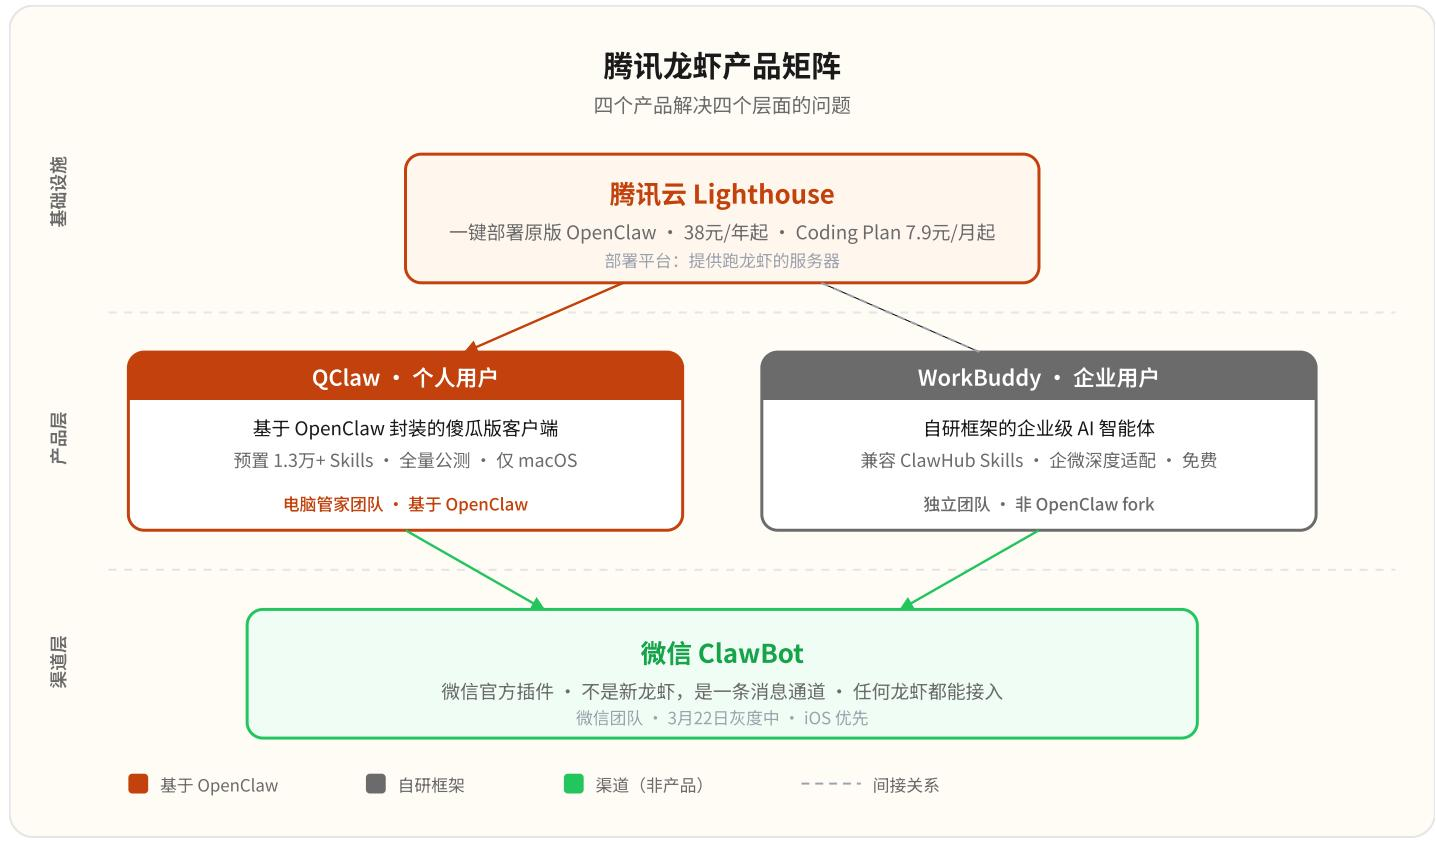
\includegraphics[keepaspectratio,alt={image}]{images/b46d83eb806e4ae0d0257987079427c601557962a57c987860716b7f58b5ee8a.jpg}}

最容易搞混的就是QClaw和ClawBot的区别：QClaw是在你电脑上装一只龙虾（产品），ClawBot是让你从微信里和已有的龙虾说话（渠道）。两者可以配合使用------用QClaw装好龙虾，再用ClawBot从手机微信远程操控它。

\section{核心建议}\label{ux6838ux5fc3ux5efaux8bae-27}

WorkBuddy 的负责人在接受采访时明确表示「WorkBuddy 不是
OpenClaw」，技术路线完全自研。但它兼容ClawHub 的 Skills
生态，用户可以直接安装社区技能。这是一个有趣的策略：自研框架 \(^ +\)
借用生态。

\section{按场景推荐}\label{ux6309ux573aux666fux63a8ux8350}

{\def\LTcaptype{none} % do not increment counter
\begin{longtable}[]{@{}|l|l|l|l|@{}}
\toprule\noalign{}
\endhead
\bottomrule\noalign{}
\endlastfoot
\hline
你的需求 & 首选 & 备选 & 理由 \\
\hline
零基础想最快体验 & AutoClaw & MaxClaw &
AutoClaw一键安装、96个预置Skills、免费起步；MaxClaw云端18秒部署、¥39/月起 \\
\hline
微信/QQ用户 & QClaw + ClawBot & WorkBuddy &
QClaw一键装好龙虾（已全量公测），ClawBot从微信远程操控；WorkBuddy自研免部署且企微整合好 \\
\hline
飞书生态 & ArkClaw & AutoClaw &
同为字节系，飞书深度适配；AutoClaw也支持飞书一键接入 \\
\hline
预算敏感 & LobsterAI & CoPaw & 两者都免费开源，自带完整功能 \\
\hline
想完全控制和深度折腾 & 原版OpenClaw & CoPaw &
开源社区最大，资源最丰富 \\
\hline
手机端+智能家居 & miclaw & - &
目前唯一的移动端方案（仅限小米17系列，封测中） \\
\hline
\end{longtable}
}

\section{注意}\label{ux6ce8ux610f-28}

选购提醒：大部分封装版产品（MaxClaw、KimiClaw等）会锁定默认模型，不能像原版OpenClaw那样自由切换。如果你对模型选择有强需求，优先考虑原版OpenClaw或支持多模型的产品（AutoClaw、WorkBuddy、LobsterAI）。另外，这些产品大多在2026年2-3月刚上线，功能和稳定性仍在快速迭代中。

\section{A 常见问题 FAQ}\label{a-ux5e38ux89c1ux95eeux9898-faq}

\section{Q1：OpenClaw是免费的吗？}\label{q1openclawux662fux514dux8d39ux7684ux5417}

OpenClaw本身是MIT开源免费的。但运行它需要两项成本：一是服务器（本地电脑或云服务器），二是AI模型的API费用。如果你用本地模型（Ollama），API费用也可以免费。总结：软件免费，算力不免费。

\section{Q2：我需要什么样的技术水平才能用OpenClaw？}\label{q2ux6211ux9700ux8981ux4ec0ux4e48ux6837ux7684ux6280ux672fux6c34ux5e73ux624dux80fdux7528openclaw}

能用命令行安装npm包就够了。最基础的安装只需要两行命令： npm install -g
openclaw@latest 和openclaw onboard -install-daemon
。如果用阿里云/腾讯云的一键部署方案，门槛更低。但如果要接入多个平台、自定义Skill、调优配置，需要一定的技术基础。

\section{Q3：OpenClaw和ChatGPT有什么区别？}\label{q3openclawux548cchatgptux6709ux4ec0ux4e48ux533aux522b}

ChatGPT是「顾问」（你问它答），OpenClaw是「员工」（它主动执行任务）。OpenClaw可以接入你的消息平台、管理邮件日历、操作浏览器、执行Shell命令，而且数据完全在你自己手上。代价是需要自己部署和维护。

\section{Q4：安全吗？我的数据会泄露吗？}\label{q4ux5b89ux5168ux5417ux6211ux7684ux6570ux636eux4f1aux6cc4ux9732ux5417}

OpenClaw是自托管的，数据默认存储在你自己的服务器上，不经过第三方。但需要注意三个安全风险：(1)CVE-2026-25253
RCE漏洞（已修复，务必更新到最新版本）；(2)
ClawHavoc供应链攻击（安装第三方Skill前务必审查源代码）；(3)
Gateway如果暴露在公网上需要设置认证（ gateway.auth.mode ）。

\section{Q5：一个月大概花多少钱？}\label{q5ux4e00ux4e2aux6708ux5927ux6982ux82b1ux591aux5c11ux94b1}

取决于你的使用方式和模型选择。参考区间：完全免费（本地模型） \$ \$ 2-5\$
/月（DeepSeek为主） \$ \$ 5 -- 15 \_ \{ I \}\$ /月（GLM-5为主） \$ \$ 10
-- 30\$
月（ClaudeSonnet为主）。最大的成本陷阱是OpenClaw的多轮工具调用会消耗大量Token，务必设置消费限额。

\section{Q6：可以用国产模型吗？效果怎么样？}\label{q6ux53efux4ee5ux7528ux56fdux4ea7ux6a21ux578bux5417ux6548ux679cux600eux4e48ux6837}

完全可以。DeepSeek-V3（\$0.14/M输入）和GLM-5（\$0.80/M输入）是最受国内用户欢迎的选择。智谱还于2026年3月16日发布了GLM-5-Turbo，这是历史上第一个从训练阶段就专为OpenClaw优化的模型，工具调用和长链执行能力专项加强，目前实验性开放。效果肯定不如ClaudeSonnet（Agent任务公认最强），但对于大部分日常任务已经够用。推荐用Fallback机制混合搭配。

\section{Q7：Anthropic封杀了OAuth，我该怎么用Claude？}\label{q7anthropicux5c01ux6740ux4e86oauthux6211ux8be5ux600eux4e48ux7528claude}

使用Anthropic API Key（按量付费）。在 Anthropic Console 创建API
Key，然后在OpenClaw中配置ANTHROPIC\_API\_KEY
环境变量。不要尝试通过OAuth连接Claude Pro/Max订阅账户，会被封号。

\section{Q8：OpenClaw创始人加入OpenAI后，项目还会继续吗？}\label{q8openclawux521bux59cbux4ebaux52a0ux5165openaiux540eux9879ux76eeux8fd8ux4f1aux7ee7ux7eedux5417}

会。Peter
Steinberger加入OpenAI后，OpenClaw正在转为开源基金会运营。OpenAI已承诺赞助项目但不干预开发方向。截至2026年3月，项目仍然保持近乎每日更新的节奏，有
\(^ { 1 , 0 7 5 + }\) 贡献者。项目的长期可持续性是有保障的。

\section{Q9：ClawHub上的Skill安全吗？}\label{q9clawhubux4e0aux7684skillux5b89ux5168ux5417}

不能盲目信任。ClawHub的13,729个Skill中，经社区审计约 \(2 0 \%\)
存在问题（垃圾/重复/恶意）。ClawHavoc事件中，超800个恶意Skill试图窃取用户凭证。建议：只安装starred数量多的Skill、安装前审查源代码、使用awesome-openclaw-skills精选列表（已过滤问题Skill）。

\section{Q10：能接入微信吗？}\label{q10ux80fdux63a5ux5165ux5faeux4fe1ux5417}

2026年3月22日之后，可以了！微信团队推出了官方插件 ClawBot，一条命令（
npx -y @tencent-weixin/openclaw-weixin-cli@latest install ） \(^ +\)
扫码即可让你的OpenClaw接入个人微信。这是官方正道，不再需要企微中转或iPad协议等灰色方案。目前ClawBot仍在灰度放量中，iOS优先（需微信
\(8 . 0 . 7 0 \cdot \mathrm { \ i }\)
），安卓时间表待定。详见本指南§17微信ClawBot。

\section{Q11：OpenClaw和Claude
Code可以一起用吗？}\label{q11openclawux548cclaude-codeux53efux4ee5ux4e00ux8d77ux7528ux5417}

可以，而且是推荐用法。社区开发了openclaw-claude-code-skill，通过MCP协议桥接两者。OpenClaw负责消息平台接入和生活自动化，ClaudeCode负责编程任务。两者组合是2026年最完整的AI工作流。

\section{Q12：本地模型效果怎么样？}\label{q12ux672cux5730ux6a21ux578bux6548ux679cux600eux4e48ux6837}

取决于硬件和模型选择。32GB
RAM可以跑Qwen3-Coder:32B或Devstral-24B，在代码生成和简单Agent任务上表现不错。但跟云端的ClaudeSonnet或GPT-5.4比仍有差距，尤其是复杂的多步骤推理任务。适合隐私敏感场景和实验用途。

\section{B 命令速查表}\label{b-ux547dux4ee4ux901fux67e5ux8868}

安装与更新

{\def\LTcaptype{none} % do not increment counter
\begin{longtable}[]{@{}|l|l|@{}}
\toprule\noalign{}
\endhead
\bottomrule\noalign{}
\endlastfoot
\hline
命令 & 说明 \\
\hline
npm install -g openclaw@latest & 全局安装OpenClaw \\
\hline
openclaw onboard -\/-install-daemon & 初始化配置+安装守护进程 \\
\hline
openclaw update -\/-channel stable & 更新到最新稳定版 \\
\hline
openclaw update -\/-channel beta & 更新到Beta版（尝鲜） \\
\hline
openclaw doctor & 诊断检查，排查常见问题 \\
\hline
openclaw -\/-version & 查看当前版本 \\
\hline
\end{longtable}
}

\section{日常使用}\label{ux65e5ux5e38ux4f7fux7528}

{\def\LTcaptype{none} % do not increment counter
\begin{longtable}[]{@{}|l|l|@{}}
\toprule\noalign{}
\endhead
\bottomrule\noalign{}
\endlastfoot
\hline
命令 & 说明 \\
\hline
openclaw gateway -\/-port 18789 -\/-verbose &
启动Gateway（详细日志模式） \\
\hline
openclaw gateway restart & 重启Gateway（改配置后必须执行） \\
\hline
openclaw agent -\/-message "xxx" & 直接发送消息给Agent \\
\hline
openclaw devices pair & 设备配对（新设备首次连接） \\
\hline
openclaw models list & 列出已配置的模型 \\
\hline
openclaw models status -\/-probe & 测试模型连通性 \\
\hline
openclaw config set agents.default.modelprimaryprovider/model &
设置主力模型 \\
\hline
/fast &
在对话中切换快速模式（v3.12新增，降低延迟，映射到模型的快速API通道） \\
\hline
openclaw backup create & 创建本地配置备份（v3.8新增） \\
\hline
openclaw backup verify & 验证备份完整性 \\
\hline
openclaw workspace trust /path & 显式信任 workspace
plugin（v3.12新增，克隆仓库不再自动加载） \\
\hline
\end{longtable}
}

\section{插件管理}\label{ux63d2ux4ef6ux7ba1ux7406}

{\def\LTcaptype{none} % do not increment counter
\begin{longtable}[]{@{}|l|l|@{}}
\toprule\noalign{}
\endhead
\bottomrule\noalign{}
\endlastfoot
\hline
命令 & 说明 \\
\hline
openclaw plugins install \textless name\textgreater{} &
安装插件/Skill \\
\hline
openclaw plugins enable \textless name\textgreater{} & 启用插件 \\
\hline
openclaw plugins list & 列出已安装插件 \\
\hline
openclaw plugins install @openclaw-china/channels & 安装中国IM插件 \\
\hline
openclaw china setup & 配置中国IM平台（需先安装插件） \\
\hline
\end{longtable}
}

\section{模型认证}\label{ux6a21ux578bux8ba4ux8bc1}

{\def\LTcaptype{none} % do not increment counter
\begin{longtable}[]{@{}|l|l|@{}}
\toprule\noalign{}
\endhead
\bottomrule\noalign{}
\endlastfoot
\hline
命令 & 说明 \\
\hline
openclaw onboard -\/-auth-choice zai-api-key & 配置智谱GLM \\
\hline
openclaw onboard -\/-auth-choice apiKey -\/-token-provider openrouter
-\/-token "\$KEY" & 配置OpenRouter \\
\hline
openclaw models auth login -\/-provider qwen-portal -\/-set-default &
通义千问OAuth登录 \\
\hline
\end{longtable}
}

\section{聊天命令（在对话中使用）}\label{ux804aux5929ux547dux4ee4ux5728ux5bf9ux8bddux4e2dux4f7fux7528}

{\def\LTcaptype{none} % do not increment counter
\begin{longtable}[]{@{}|l|l|@{}}
\toprule\noalign{}
\endhead
\bottomrule\noalign{}
\endlastfoot
\hline
命令 & 说明 \\
\hline
/status & 会话概览（当前模型、Token用量） \\
\hline
/new & 清空会话历史，开始新对话 \\
\hline
/think \textless level\textgreater{} &
调整推理深度（off/minimal/low/medium/high/xhigh） \\
\hline
/usage off\textbar tokens\textbar full & 控制回复页脚的用量显示 \\
\hline
/activation mention\textbar always & 群消息处理模式 \\
\hline
\end{longtable}
}

\section{Docker部署}\label{dockerux90e8ux7f72}

{\def\LTcaptype{none} % do not increment counter
\begin{longtable}[]{@{}|l|l|@{}}
\toprule\noalign{}
\endhead
\bottomrule\noalign{}
\endlastfoot
\hline
命令 & 说明 \\
\hline
docker-compose up -d & 后台启动OpenClaw容器 \\
\hline
docker-compose logs -f & 查看实时日志 \\
\hline
docker-compose pull \&\& docker-compose up -d & 更新到最新镜像 \\
\hline
\end{longtable}
}

\section{C 资源链接}\label{c-ux8d44ux6e90ux94feux63a5}

官方资源

{\def\LTcaptype{none} % do not increment counter
\begin{longtable}[]{@{}|l|l|@{}}
\toprule\noalign{}
\endhead
\bottomrule\noalign{}
\endlastfoot
\hline
资源 & 地址 \\
\hline
GitHub仓库 & github.com/openclaw/openclaw \\
\hline
官方文档 & docs.openclaw.ai \\
\hline
官网 & openclaw.ai \\
\hline
ClawHub技能市场 & clawhub.ai \\
\hline
Moltbook (Agent社交网络) & moltbook.com \\
\hline
GitHub Releases & github.com/openclaw/openclaw/releases \\
\hline
GitHub Discussions & github.com/openclaw/openclaw/discussions \\
\hline
\end{longtable}
}

社区资源

{\def\LTcaptype{none} % do not increment counter
\begin{longtable}[]{@{}|l|l|l|@{}}
\toprule\noalign{}
\endhead
\bottomrule\noalign{}
\endlastfoot
\hline
资源 & 地址 & 说明 \\
\hline
awesome-openclaw-skills & github.com/VoltAgent/awesome-openclaw-skills &
5,494个精选Skill（已过滤问题Skill），31.4K Stars \\
\hline
awesome-openclaw-usecases &
github.com/hesamsheikh/awesome-openclaw-usecases & 社区用例合集，21K
Stars \\
\hline
openclaw-claude-code-skill &
github.com/Enderfga/openclaw-claude-code-skill & 桥接Claude Code能力 \\
\hline
SecureClaw & 开源安全工具 & Skill安全扫描 \\
\hline
\end{longtable}
}

国内资源

{\def\LTcaptype{none} % do not increment counter
\begin{longtable}[]{@{}|l|l|l|@{}}
\toprule\noalign{}
\endhead
\bottomrule\noalign{}
\endlastfoot
\hline
资源 & 地址 & 说明 \\
\hline
openclaw-china插件 & github.com/BytePioneer-AI/openclaw-china &
钉钉/QQ/企微/微信接入 \\
\hline
OpenClaw中文文档 & openclaw.cc & 社区维护的中文文档 \\
\hline
阿里云部署文档 & help.aliyun.com（搜索OpenClaw） &
轻量应用服务器一键部署 \\
\hline
B站部署教程 & BV1MfAz6EnR & 保姆级：接入微信/飞书/钉钉/QQ \\
\hline
\end{longtable}
}

教程资源

{\def\LTcaptype{none} % do not increment counter
\begin{longtable}[]{@{}|l|l|l|@{}}
\toprule\noalign{}
\endhead
\bottomrule\noalign{}
\endlastfoot
\hline
资源 & 语言 & 说明 \\
\hline
freeCodeCamp完整教程 & 英文 & 从零开始的完整指南 \\
\hline
DigitalOcean介绍 & 英文 & What is OpenClaw概述 \\
\hline
知乎部署系列 & 中文 & 多篇部署和使用教程 \\
\hline
博客园源码编译指南 & 中文 & 从源码构建OpenClaw \\
\hline
菜鸟教程一键部署 & 中文 & 最简部署方案 \\
\hline
\end{longtable}
}

模型提供商

{\def\LTcaptype{none} % do not increment counter
\begin{longtable}[]{@{}|l|l|@{}}
\toprule\noalign{}
\endhead
\bottomrule\noalign{}
\endlastfoot
\hline
提供商 & API控制台 \\
\hline
Anthropic Claude & consoleanthropic.com \\
\hline
OpenAI & platform.openai.com \\
\hline
Google AI Studio & aistudio.google.com \\
\hline
DeepSeek & platform\_deepseek.com \\
\hline
智谱GLM & bigmodel.cn \\
\hline
通义千问 & dashscope.aliyun.com \\
\hline
月之暗面Kimi & platform.moonshot.cn \\
\hline
硅基流动 & siliconflow.cn \\
\hline
OpenRouter & openrouter.ai \\
\hline
火山引擎（豆包） & console.volcengine.com \\
\hline
\end{longtable}
}

本文档在ClaudeCode辅助下整理编写，基于OpenClaw官方文档、GitHub仓库及社区资料。

内容的准确性与时效性仅供参考，如有勘误或建议，欢迎关注公众号「花叔」反馈交流。

来源：docs.openclaw.ai · github.com/openclaw/openclaw · clawhub.com ·
Created by 花叔 · 2026 年 3 月

\section{AI编程：从入门到精通}\label{aiux7f16ux7a0bux4eceux5165ux95e8ux5230ux7cbeux901a}

知识星球· 花叔的AI编程社区

\pandocbounded{
\includegraphics[keepaspectratio,alt={image}]{images/ef93289aee8f4e2e0a75b9107e1364c1134747f3575a05974c0291bd6797a473.jpg}}

知识星球二维码

\section{星主：AI进化论-花生}\label{ux661fux4e3baiux8fdbux5316ux8bba-ux82b1ux751f}

自然语言是AI时代最好的编程语言。

AppStore付费app总榜第一「小猫补光灯」作者

《一本书玩转 DeepSeek》作者

加入知识星球→

B站：AI进化论-花生 YouTube：AI进化论-花生 公众号：花叔

Created by 花叔 · v1.1 · 2026年3月

配套视频：B站「OpenClaw从0到1」 · 后续更新：飞书文档

\end{document}
